\documentclass[aspectratio=169,11pt]{beamer}

\usepackage{tikz}
\usepackage{pgfplots}
\pgfplotsset{compat=1.18}
\usepackage[T1]{fontenc}
\usepackage[utf8]{inputenc}
\usepackage{booktabs}
\usepackage{xcolor}
\usepackage{amsmath}
\usepackage{fontawesome5}
\usetikzlibrary{shapes.geometric,arrows.meta,positioning,calc,decorations.pathmorphing,patterns,backgrounds,fit}

\providecommand{\faCompressArrowsAlt}{\faCompress}

\def\PaletteChoice{1}

\ifnum\PaletteChoice=1
  \definecolor{PA}{HTML}{0D3B66}
  \definecolor{PB}{HTML}{2D9CDB}
  \definecolor{PC}{HTML}{56CCF2}
  \definecolor{PD}{HTML}{F2A900}
  \definecolor{PE}{HTML}{56CCF2}
  \definecolor{PF}{HTML}{0D3B66}
  \definecolor{PG}{HTML}{1A5E8A}
  \definecolor{PH}{HTML}{F4F8FC}
  \definecolor{PI}{HTML}{D6EAF8}
\fi

\setbeamercolor{structure}{fg=PB}
\setbeamercolor{palette primary}{bg=PA, fg=PH}
\setbeamercolor{palette secondary}{bg=PG, fg=PH}
\setbeamercolor{palette tertiary}{bg=PA, fg=PH}
\setbeamercolor{title}{fg=PA, bg=PD}
\setbeamercolor{frametitle}{fg=PH, bg=PA}
\setbeamercolor{section in head/foot}{bg=PA, fg=PH}
\setbeamercolor{subsection in head/foot}{bg=PG, fg=PH}
\setbeamercolor{background canvas}{bg=PH}
\setbeamercolor{normal text}{fg=PF}
\setbeamercolor{frametitle}{fg=PH, bg=PA}
\setbeamercolor{itemize item}{fg=PB}
\setbeamercolor{itemize subitem}{fg=PE}
\setbeamercolor{block title}{bg=PA, fg=PH}
\setbeamercolor{block body}{bg=PI!50, fg=PF}
\setbeamercolor{block title alerted}{bg=PB, fg=PH}
\setbeamercolor{block body alerted}{bg=PI!40, fg=PF}
\setbeamercolor{footer bar}{bg=PF, fg=PH!80}
\setbeamerfont{frametitle}{size=\large,series=\bfseries}
\setbeamerfont{block title}{series=\bfseries}
\setbeamertemplate{navigation symbols}{}


% ---- HEADER ----
\setbeamertemplate{frametitle}{%
  \begin{tikzpicture}[remember picture,overlay]
    \fill[PA] (current page.north west)
      rectangle ([yshift=-1.15cm] current page.north east);
    \fill[PB]
      ([xshift=11.5cm] current page.north west) --
      ([xshift=12.5cm] current page.north west) --
      ([xshift=12.5cm,yshift=-1.15cm] current page.north west) --
      ([xshift=11.0cm,yshift=-1.15cm] current page.north west) -- cycle;
    \fill[PD]
      ([yshift=-1.15cm] current page.north west)
      rectangle ([yshift=-1.28cm] current page.north east);
    \node[anchor=west,text=PH,font=\large\bfseries]
      at ([xshift=0.45cm,yshift=-0.57cm] current page.north west)
      {\insertframetitle};
  \end{tikzpicture}%
  \vspace{0.95cm}%
}
\setbeamertemplate{footline}{%
  \begin{tikzpicture}[remember picture,overlay]
    \fill[PF] (current page.south west)
      rectangle ([yshift=0.4cm] current page.south east);
    \node[anchor=center,text=PH!80,font=\tiny]
      at ([yshift=0.2cm] current page.south)
      {Bangladesh University of Engineering and Technology \textbullet\ Convolutional Neural Network \textbullet\ \insertshortdate\ \textbullet\ \insertframenumber\,/\,\inserttotalframenumber};
  \end{tikzpicture}%
}
% ---- BULLETS ----
\setbeamertemplate{itemize item}{%
  \tikz{\fill[PB] (0,0.05)--(0.2,0.1)--(0,0.2)--(0.05,0.12)--cycle;}%
}
\setbeamertemplate{itemize subitem}{%
  \tikz{\fill[PE,rotate=45](-0.07,-0.07) rectangle (0.07,0.07);}%
}

%% Cell size constants
\def\CS{0.52}
\def\CSG{0.54}

%% Basic cell
\newcommand{\gc}[5]{%
  \fill[#4](\fpeval{(#1)*\CSG},\fpeval{-(#2)*\CSG})
    rectangle ++(\CS,\CS);
  \draw[PA!20,line width=0.2pt](\fpeval{(#1)*\CSG},\fpeval{-(#2)*\CSG})
    rectangle ++(\CS,\CS);
  \node[font=\scriptsize\bfseries,text=#5]
    at (\fpeval{(#1)*\CSG+\CS/2},\fpeval{-(#2)*\CSG+\CS/2}){#3};
}

%% 3×3 Sobel-X kernel
\newcommand{\sobelK}{%
  \gc{0}{0}{ 1}{PB!55}{white}%
  \gc{1}{0}{ 0}{PI!60}{PF}%
  \gc{2}{0}{-1}{PD!55}{white}%
  \gc{0}{1}{ 2}{PB!75}{white}%
  \gc{1}{1}{ 0}{PI!60}{PF}%
  \gc{2}{1}{-2}{PD!75}{white}%
  \gc{0}{2}{ 1}{PB!55}{white}%
  \gc{1}{2}{ 0}{PI!60}{PF}%
  \gc{2}{2}{-1}{PD!55}{white}%
}

%% 5×5 input with highlighted window
\newcommand{\inputW}[2]{%
  \foreach \cc/\rr/\vv in {%
    0/0/3,1/0/1,2/0/0,3/0/2,4/0/4,%
    0/1/1,1/1/5,2/1/2,3/1/0,4/1/3,%
    0/2/0,1/2/2,2/2/4,3/2/1,4/2/2,%
    0/3/3,1/3/1,2/3/0,3/3/3,4/3/1,%
    0/4/1,1/4/0,2/4/2,3/4/1,4/4/4%
  }{%
    \pgfmathtruncatemacro\inwin{(\cc>=#1)*(\cc<#1+3)*(\rr>=#2)*(\rr<#2+3)}%
    \ifnum\inwin=1
      \gc{\cc}{\rr}{\vv}{PB!50}{white}%
    \else
      \gc{\cc}{\rr}{\vv}{PI!65}{PF!80}%
    \fi
  }%
  \draw[PD,line width=1.8pt,rounded corners=1.2pt]
    (\fpeval{#1*\CSG-0.02},\fpeval{-#2*\CSG+\CS+0.02})
    rectangle
    ++(\fpeval{3*\CSG-0.02},\fpeval{-3*\CSG-0.02});%
}

%% Filled output cell
\newcommand{\oc}[4]{%
  \fill[#4](\fpeval{#1*\CSG},\fpeval{-#2*\CSG}) rectangle ++(\CS,\CS);
  \draw[PD!50,line width=0.5pt](\fpeval{#1*\CSG},\fpeval{-#2*\CSG})
    rectangle ++(\CS,\CS);
  \node[font=\scriptsize\bfseries,white]
    at (\fpeval{#1*\CSG+\CS/2},\fpeval{-#2*\CSG+\CS/2}){#3};
}

%% Empty output cell
\newcommand{\ocE}[2]{%
  \fill[PI!35](\fpeval{#1*\CSG},\fpeval{-#2*\CSG}) rectangle ++(\CS,\CS);
  \draw[PA!15,line width=0.3pt](\fpeval{#1*\CSG},\fpeval{-#2*\CSG})
    rectangle ++(\CS,\CS);
}

%% MAIN SLIDE MACRO
\newcommand{\simslide}[8]{%
\centering
\begin{tikzpicture}[scale=1.0, baseline=(current bounding box.north)]
  \node[font=\footnotesize\bfseries,PA]
    at (1.35, \fpeval{\CS+0.55}){Input ($5{\times}5$)};
  \node[font=\footnotesize\bfseries,PB]
    at (3.86, \fpeval{\CS+0.55}){Kernel};
  \node[font=\footnotesize\bfseries,PA]
    at (5.82, \fpeval{\CS+0.55}){Result};
  \node[font=\footnotesize\bfseries,#6]
    at (8.60, \fpeval{\CS+0.55}){#7};
  \inputW{#1}{#2}
  \node[font=\large\bfseries,PA]
    at (\fpeval{5*\CSG + 0.18}, \fpeval{-\CS}){$\times$};
  \begin{scope}[xshift=\fpeval{5*\CSG + 0.35} cm, yshift=\fpeval{-\CS*0.5} cm]
    \sobelK
  \end{scope}
  \node[font=\large\bfseries,PA]
    at (\fpeval{5*\CSG + 0.35 + 3*\CSG + 0.3}, \fpeval{-\CS}){$=$};
  \node[draw=PD,fill=PI!30,rounded corners=3pt,
        font=\normalsize\bfseries,text=PA,
        minimum width=1.1cm,minimum height=0.72cm]
    at (\fpeval{5*\CSG + 0.35 + 3*\CSG + 0.6 + 0.55}, \fpeval{-\CS}){$#3$};
  \node[font=\tiny,PG]
    at (\fpeval{5*\CSG + 0.35 + 3*\CSG + 0.6 + 0.55}, \fpeval{-\CS - 0.5}){$#4$};
  \draw[->,PA,thick]
    (\fpeval{5*\CSG + 0.35 + 3*\CSG + 0.6 + 1.15}, \fpeval{-\CS})
    -- ++( 0.35, 0);
  \begin{scope}[xshift=\fpeval{5*\CSG + 0.35 + 3*\CSG + 0.6 + 0.7 + 3*\CSG + 0.2} cm,
                yshift=\fpeval{-\CS*0.5} cm]
    #8
  \end{scope}
\end{tikzpicture}

\vspace{4pt}
\begin{tikzpicture}
  \node[fill=PI!50,draw=PA!25,rounded corners=3pt,
        font=\fontsize{6.2}{8}\selectfont,text=PF,align=center,
        minimum width=13.5cm,minimum height=0.55cm,inner sep=3pt] at (0,0){#5};
\end{tikzpicture}
}

\newcommand{\relucell}[4]{%
  \pgfmathtruncatemacro\isneg{(#3<0)?1:0}%
  \ifnum\isneg=1
    \gc{#1}{#2}{#4}{PD!60}{white}%
  \else
    \gc{#1}{#2}{#4}{PB!65}{white}%
  \fi
}

\institute{Bangladesh University of Engineering and Technology}
\date{February 2026}
\title[Convolutional Neural Network]{The Convolution Layer}

\begin{document}
% \setbeamercolor{background canvas}{bg=PA}
% \begin{frame}[plain, noframenumbering]
% \centering
% \vfill
%   {\color{PD}\fontsize{24}{30}\selectfont\bfseries
%     Convolutional Neural Networks}\\[8pt]
%   {\color{PC}\large
%     How Machines Learn to See}\\[12pt]
%   {\color{PD}\rule{9cm}{1pt}}\\[10pt]
% \vfill
% \end{frame}
% \setbeamercolor{background canvas}{bg=white}
\setbeamercolor{background canvas}{bg=PA}
\begin{frame}[plain, noframenumbering]
\begin{tikzpicture}[remember picture, overlay]

  %% ── Background base ──────────────────────────────────────────
  \fill[PA] (current page.south west) rectangle (current page.north east);

  %% ── Top-left glowing circle cluster ─────────────────────────
  \fill[PB, opacity=0.18] ([xshift=-2cm, yshift=-2cm] current page.north west) circle (5.5cm);
  \fill[PB, opacity=0.28] ([xshift=-2cm, yshift=-2cm] current page.north west) circle (3.2cm);
  \fill[PC, opacity=0.12] ([xshift=-2cm, yshift=-2cm] current page.north west) circle (1.8cm);

  %% ── Bottom-right warm accent triangle ────────────────────────
  \fill[PD, opacity=0.80]
    ([xshift=16cm] current page.south west) --
    ([xshift=16cm, yshift=6cm] current page.south west) --
    ([xshift=10cm] current page.south west) -- cycle;
  \fill[PE, opacity=0.55]
    ([xshift=15.0cm] current page.south west)
    rectangle (current page.north east);

  %% ── Mid diagonal parallelogram (depth layer) ─────────────────
  \fill[PC, opacity=0.07]
    ([xshift=3.5cm, yshift=0.8cm] current page.south west) --
    ([xshift=9.5cm, yshift=0.8cm] current page.south west) --
    ([xshift=7.5cm, yshift=8.5cm] current page.south west) --
    ([xshift=1.5cm, yshift=8.5cm] current page.south west) -- cycle;

  %% ── Abstract neural-net node grid (top-right) ────────────────
  \foreach \nx in {11.5, 12.3, 13.1, 13.9, 14.7}{
    \foreach \ny in {5.5, 6.3, 7.1, 7.9}{
      \fill[PB, opacity=0.18] (\nx, \ny) circle (2.5pt);
    }
  }
  %% Connect nodes horizontally
  \foreach \ny in {5.5, 6.3, 7.1, 7.9}{
    \draw[PB, opacity=0.12, line width=0.6pt]
      (11.5, \ny) -- (14.7, \ny);
  }
  %% Connect nodes vertically
  \foreach \nx in {11.5, 12.3, 13.1, 13.9, 14.7}{
    \draw[PB, opacity=0.12, line width=0.6pt]
      (\nx, 5.5) -- (\nx, 7.9);
  }
  %% Highlight a few nodes
  \fill[PC, opacity=0.65] (12.3, 6.3) circle (4pt);
  \fill[PD, opacity=0.80] (13.1, 7.1) circle (5pt);
  \fill[PC, opacity=0.50] (13.9, 6.3) circle (3.5pt);

  %% ── Amber horizontal rule (left edge accent) ─────────────────
  \fill[PD]
    ([xshift=3.8cm, yshift=3.55cm] current page.south west)
    rectangle ([xshift=14.8cm, yshift=3.75cm] current page.south west);

  %% ── Main title ───────────────────────────────────────────────
  \node[anchor=west, text=PH,
        font=\fontsize{28}{34}\selectfont\bfseries,
        text width=11cm]
    at ([xshift=3.9cm, yshift=5.0cm] current page.south west)
    {Convolutional\\Neural Networks};

  %% ── Subtitle ─────────────────────────────────────────────────
  \node[anchor=west, text=PC,
        font=\fontsize{12.5}{16}\selectfont]
    at ([xshift=3.9cm, yshift=3.05cm] current page.south west)
    {How Machines Learn to See};

  %% ── Institute + date tag ─────────────────────────────────────
 %% ── Author names ─────────────────────────────────────────────
  \node[anchor=west, text=PH!70,
        font=\fontsize{9.5}{10}\selectfont\bfseries]
    at ([xshift=3.6cm, yshift=2.25cm] current page.south west)
    {Arjo Kar \quad\textbullet\quad Lamisa Zahin \quad\textbullet\quad Zannatun Nayeem Ohee};

  %% ── Bottom rainbow bar (matches other slides) ─────────────────
  \fill[PA]  (current page.south west)
    rectangle ([xshift=2.28cm, yshift=0.55cm] current page.south west);
  \fill[PB]  ([xshift=2.30cm] current page.south west)
    rectangle ([xshift=4.58cm, yshift=0.55cm] current page.south west);
  \fill[PC]  ([xshift=4.60cm] current page.south west)
    rectangle ([xshift=6.88cm, yshift=0.55cm] current page.south west);
  \fill[PD]  ([xshift=6.90cm] current page.south west)
    rectangle ([xshift=9.18cm, yshift=0.55cm] current page.south west);
  \fill[PE]  ([xshift=9.20cm] current page.south west)
    rectangle ([xshift=11.48cm, yshift=0.55cm] current page.south west);
  \fill[PG]  ([xshift=11.50cm] current page.south west)
    rectangle ([xshift=13.78cm, yshift=0.55cm] current page.south west);
  \fill[PF]  ([xshift=13.80cm] current page.south west)
    rectangle ([xshift=16.08cm, yshift=0.55cm] current page.south west);

\end{tikzpicture}
\end{frame}
\setbeamercolor{background canvas}{bg=white}
%% ════════════════════════════════════════════════════════
%%  SLIDE 2a – STORY : THE PROBLEM
%% ════════════════════════════════════════════════════════
\begin{frame}{The Story Behind CNN}
\vspace{4pt}

\begin{columns}[T]

\begin{column}{0.30\textwidth}
\centering
\vspace{8pt}

  \begin{tikzpicture}[
    spot/.style={draw=PB, fill=PB!12,
                 rounded corners=4pt,
                 minimum width=2.4cm,
                 minimum height=0.62cm,
                 font=\footnotesize\bfseries,
                 text=PB, align=center,
                 line width=2pt},
    next/.style={draw=PA!20, fill=PA!4,
                 rounded corners=4pt,
                 minimum width=2.4cm,
                 minimum height=0.62cm,
                 font=\footnotesize\bfseries,
                 text=PA!30, align=center},
    arr/.style={->, line width=1.2pt, color=PA!20}
  ]
    \node[spot] (s1) at (0,  0.00)
      {\faMedkit\; The Problem};
    \draw[arr] (s1.south) -- ++(0,-0.38);
    \node[next] (s2) at (0, -1.00)
      {\faUserMd\; Naive Doctor};
    \draw[arr] (s2.south) -- ++(0,-0.38);
    \node[next] (s3) at (0, -2.00)
      {\faLightbulb\; The Insight};
    \draw[arr] (s3.south) -- ++(0,-0.38);
    \node[next] (s4) at (0, -3.00)
      {\faBrain\; CNN Solution};
  \end{tikzpicture}

\end{column}

\begin{column}{0.66\textwidth}
\vspace{8pt}

  {\color{PB}\footnotesize\bfseries
    \faMedkit\; Step 1 of 4 --
    \underline{The Problem}}\\[10pt]

  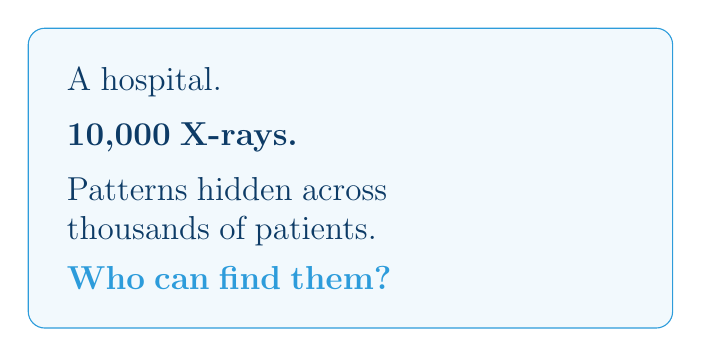
\begin{tikzpicture}
    \node[draw=PB, fill=PB!6,
          rounded corners=6pt,
          text width=7.2cm,
          inner sep=14pt] {
      \color{PA}
      \large
      A hospital.\\[6pt]
      \textbf{10,000 X-rays.}\\[6pt]
      Patterns hidden across\\
      thousands of patients.\\[6pt]
      {\color{PB}\bfseries
        Who can find them?}
    };
  \end{tikzpicture}

\end{column}
\end{columns}
\end{frame}
%% ════════════════════════════════════════════════════════
%%  SLIDE – NAIVE DOCTOR  (fixed)
%% ════════════════════════════════════════════════════════
\begin{frame}{The Story Behind CNN}
\vspace{4pt}
\begin{columns}[T]

\begin{column}{0.30\textwidth}
\centering\vspace{8pt}
  \begin{tikzpicture}[
    done/.style={draw=PA!30, fill=PA!5,
                 rounded corners=4pt, minimum width=2.4cm,
                 minimum height=0.62cm, font=\footnotesize\bfseries,
                 text=PA!40, align=center},
    spot/.style={draw=red, fill=red!8, rounded corners=4pt,
                 minimum width=2.4cm, minimum height=0.62cm,
                 font=\footnotesize\bfseries, text=red,
                 align=center, line width=2pt},
    next/.style={draw=PA!20, fill=PA!4,
                 rounded corners=4pt, minimum width=2.4cm,
                 minimum height=0.62cm, font=\footnotesize\bfseries,
                 text=PA!30, align=center},
    arr/.style={->, line width=1.2pt, color=PA!20},
    sarr/.style={->, line width=1.8pt, color=red}
  ]
    \node[done] (s1) at (0, 0.00) {\faMedkit\; The Problem};
    \draw[sarr] (s1.south) -- ++(0,-0.38);
    \node[spot] (s2) at (0,-1.00) {\faUserMd\; Naive Doctor};
    \draw[arr]  (s2.south) -- ++(0,-0.38);
    \node[next] (s3) at (0,-2.00) {\faLightbulb\; The Insight};
    \draw[arr]  (s3.south) -- ++(0,-0.38);
    \node[next] (s4) at (0,-3.00) {\faBrain\; CNN Solution};
  \end{tikzpicture}
\end{column}

\begin{column}{0.66\textwidth}
\vspace{6pt}
  {\color{PA}\footnotesize\bfseries
    \faUserMd\; Step 2 of 4 -- \underline{The Naive Doctor}}\\[8pt]

  \begin{columns}[T]

    \begin{column}{0.34\textwidth}
      \begin{tikzpicture}
        \node[draw=PA, fill=PA!5, rounded corners=6pt,
              text width=2.5cm, inner sep=9pt] {
          \footnotesize\color{PA}
          Sees scan 1.\\[4pt]
          {\color{PA}\faTimes}\; Forgets it.\\[6pt]
          Sees scan 2.\\[4pt]
          {\color{PA}\faTimes}\; Forgets it.\\[6pt]
          {\color{PA}\bfseries
            No memory.\\[2pt]No pattern.}
        };
      \end{tikzpicture}
    \end{column}

    \begin{column}{0.30\textwidth}
    \centering
      {\fontsize{7.5}{7.5}\selectfont\bfseries\color{PA}
        Scan 1}\\[4pt]
      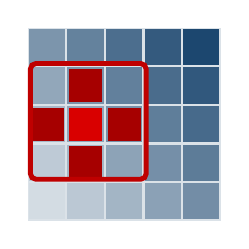
\begin{tikzpicture}[scale=0.70]
        \foreach \c in {0,...,4}{
          \foreach \r in {0,...,4}{
            \pgfmathtruncatemacro{\g}{18+\c*10+\r*9}
            \fill[PA!\g!white]
              (\c*0.70,\r*0.70) rectangle ++(0.68,0.68);
            \draw[PA!15]
              (\c*0.70,\r*0.70) rectangle ++(0.68,0.68);
          }
        }
        \fill[red!85!black] (1*0.70+0.04,2*0.70+0.04)
          rectangle ++(0.60,0.60);
        \fill[red!65!black] (1*0.70+0.04,3*0.70+0.04)
          rectangle ++(0.60,0.60);
        \fill[red!65!black] (1*0.70+0.04,1*0.70+0.04)
          rectangle ++(0.60,0.60);
        \fill[red!65!black] (2*0.70+0.04,2*0.70+0.04)
          rectangle ++(0.60,0.60);
        \fill[red!65!black] (0*0.70+0.04,2*0.70+0.04)
          rectangle ++(0.60,0.60);
        \draw[red!75!black, line width=1.8pt, rounded corners=2pt]
          (0.04,0.74) rectangle ++(2.10,2.10);
      \end{tikzpicture}
    \end{column}

    \begin{column}{0.08\textwidth}
    \centering\vspace{26pt}
      {\color{PA}\Large\bfseries\faTimes}
    \end{column}

    \begin{column}{0.28\textwidth}
    \centering
      {\fontsize{7.5}{7.5}\selectfont\bfseries\color{PA}
        Scan 2}\\[4pt]
      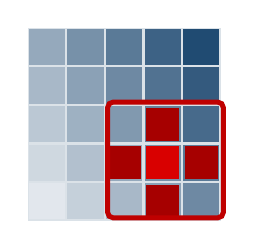
\begin{tikzpicture}[scale=0.70]
        \foreach \c in {0,...,4}{
          \foreach \r in {0,...,4}{
            \pgfmathtruncatemacro{\g}{12+\c*12+\r*8}
            \fill[PA!\g!white]
              (\c*0.70,\r*0.70) rectangle ++(0.68,0.68);
            \draw[PA!15]
              (\c*0.70,\r*0.70) rectangle ++(0.68,0.68);
          }
        }
        \fill[red!85!black] (3*0.70+0.04,1*0.70+0.04)
          rectangle ++(0.60,0.60);
        \fill[red!65!black] (3*0.70+0.04,2*0.70+0.04)
          rectangle ++(0.60,0.60);
        \fill[red!65!black] (3*0.70+0.04,0*0.70+0.04)
          rectangle ++(0.60,0.60);
        \fill[red!65!black] (4*0.70+0.04,1*0.70+0.04)
          rectangle ++(0.60,0.60);
        \fill[red!65!black] (2*0.70+0.04,1*0.70+0.04)
          rectangle ++(0.60,0.60);
        \draw[red!75!black, line width=1.8pt, rounded corners=2pt]
          (1.44,0.04) rectangle ++(2.10,2.10);
      \end{tikzpicture}
    \end{column}

  \end{columns}

  \vspace{8pt}
  
\begin{tikzpicture}
    \node[draw=PA!40, fill=PA!4, rounded corners=4pt,
          text width=7.4cm, inner sep=6pt,
          font=\fontsize{7.5}{7.5}\selectfont\itshape\color{PA},
          align=center] {
      {\color{PA}
        same pattern -- different position --
        completely missed.}
    };
  \end{tikzpicture}

\end{column}
\end{columns}
\end{frame}

%% ════════════════════════════════════════════════════════
%%  SLIDE – THE INSIGHT  (fixed)
%% ════════════════════════════════════════════════════════
\begin{frame}{The Story Behind CNN}
\vspace{4pt}
\begin{columns}[T]

\begin{column}{0.30\textwidth}
\centering\vspace{8pt}
  \begin{tikzpicture}[
    done/.style={draw=PA!30, fill=PA!5,
                 rounded corners=4pt, minimum width=2.4cm,
                 minimum height=0.62cm, font=\footnotesize\bfseries,
                 text=PA!40, align=center},
    spot/.style={draw=PD, fill=PD!8, rounded corners=4pt,
                 minimum width=2.4cm, minimum height=0.62cm,
                 font=\footnotesize\bfseries, text=PD,
                 align=center, line width=2pt},
    next/.style={draw=PA!20, fill=PA!4,
                 rounded corners=4pt, minimum width=2.4cm,
                 minimum height=0.62cm, font=\footnotesize\bfseries,
                 text=PA!30, align=center},
    arr/.style={->, line width=1.2pt, color=PA!20},
    sarr/.style={->, line width=1.8pt, color=PD}
  ]
    \node[done] (s1) at (0, 0.00) {\faMedkit\; The Problem};
    \draw[arr]  (s1.south) -- ++(0,-0.38);
    \node[done] (s2) at (0,-1.00) {\faUserMd\; Naive Doctor};
    \draw[sarr] (s2.south) -- ++(0,-0.38);
    \node[spot] (s3) at (0,-2.00) {\faLightbulb\; The Insight};
    \draw[arr]  (s3.south) -- ++(0,-0.38);
    \node[next] (s4) at (0,-3.00) {\faBrain\; CNN Solution};
  \end{tikzpicture}
\end{column}

\begin{column}{0.66\textwidth}
\vspace{6pt}
  {\color{PD}\footnotesize\bfseries
    \faLightbulb\; Step 3 of 4 -- \underline{The Insight}}\\[8pt]

  \begin{columns}[T]

    \begin{column}{0.34\textwidth}
      \begin{tikzpicture}
        \node[draw=PD, fill=PD!6, rounded corners=6pt,
              text width=2.5cm, inner sep=9pt] {
          \footnotesize\color{PA}
          Experienced doctor sees scan 1.\\[4pt]
          {\color{green!60!black}\faCheck}\;
          Remembers the pattern.\\[4pt]
          Scan 2 matches.\\[4pt]
          {\color{PD}\bfseries Recognised!}
        };
      \end{tikzpicture}
    \end{column}

    \begin{column}{0.28\textwidth}
    \centering
      {\fontsize{7.5}{7.5}\selectfont\bfseries\color{PA}
        Scan 1}\\[4pt]
      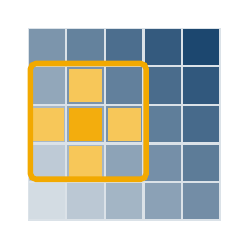
\begin{tikzpicture}[scale=0.70]
        \foreach \c in {0,...,4}{
          \foreach \r in {0,...,4}{
            \pgfmathtruncatemacro{\g}{18+\c*10+\r*9}
            \fill[PA!\g!white]
              (\c*0.70,\r*0.70) rectangle ++(0.68,0.68);
            \draw[PA!15]
              (\c*0.70,\r*0.70) rectangle ++(0.68,0.68);
          }
        }
        \fill[PD!95] (1*0.70+0.04,2*0.70+0.04)
          rectangle ++(0.60,0.60);
        \fill[PD!65] (1*0.70+0.04,3*0.70+0.04)
          rectangle ++(0.60,0.60);
        \fill[PD!65] (1*0.70+0.04,1*0.70+0.04)
          rectangle ++(0.60,0.60);
        \fill[PD!65] (2*0.70+0.04,2*0.70+0.04)
          rectangle ++(0.60,0.60);
        \fill[PD!65] (0*0.70+0.04,2*0.70+0.04)
          rectangle ++(0.60,0.60);
        \draw[PD, line width=2pt, rounded corners=2pt]
          (0.04,0.74) rectangle ++(2.10,2.10);
      \end{tikzpicture}
    \end{column}

    \begin{column}{0.10\textwidth}
    \centering\vspace{26pt}
      
\begin{tikzpicture}
        \draw[->, line width=1.8pt, PD]
          (0,0) -- (0.56,0);
        \node[above, font=\fontsize{5.5}{5.5}
              \selectfont\bfseries, color=PD]
          at (0.28,0.02) {memory};
      \end{tikzpicture}
    \end{column}

    \begin{column}{0.28\textwidth}
    \centering
      {\fontsize{7.5}{7.5}\selectfont\bfseries\color{PA}
        Scan 2}\\[4pt]
      \begin{tikzpicture}[scale=0.70]
        \foreach \c in {0,...,4}{
          \foreach \r in {0,...,4}{
            \pgfmathtruncatemacro{\g}{12+\c*12+\r*8}
            \fill[PA!\g!white]
              (\c*0.70,\r*0.70) rectangle ++(0.68,0.68);
            \draw[PA!15]
              (\c*0.70,\r*0.70) rectangle ++(0.68,0.68);
          }
        }
        \fill[PD!95] (3*0.70+0.04,1*0.70+0.04)
          rectangle ++(0.60,0.60);
        \fill[PD!65] (3*0.70+0.04,2*0.70+0.04)
          rectangle ++(0.60,0.60);
        \fill[PD!65] (3*0.70+0.04,0*0.70+0.04)
          rectangle ++(0.60,0.60);
        \fill[PD!65] (4*0.70+0.04,1*0.70+0.04)
          rectangle ++(0.60,0.60);
        \fill[PD!65] (2*0.70+0.04,1*0.70+0.04)
          rectangle ++(0.60,0.60);
        \draw[PD, line width=2pt, rounded corners=2pt]
          (1.44,0.04) rectangle ++(2.10,2.10);
        \node[font=\large\bfseries, color=green!60!black]
          at (2.49,0.74) {\faCheck};
      \end{tikzpicture}
    \end{column}

  \end{columns}

  \vspace{8pt}
  
\begin{tikzpicture}
    \node[draw=PD, fill=PD!8, rounded corners=4pt,
          text width=7.4cm, inner sep=6pt,
          font=\fontsize{7.5}{7.5}\selectfont\color{PA},
          align=center] {
      {\color{PD}\bfseries\faCheck\;}
      Same cross pattern -- different position --
      recognised instantly.
    };
  \end{tikzpicture}

\end{column}
\end{columns}
\end{frame}
%% ════════════════════════════════════════════════════════
%%  SLIDE 2d – STORY : CNN IS THE ANSWER
%% ════════════════════════════════════════════════════════
\begin{frame}{The Story Behind CNN}
\vspace{4pt}

\begin{columns}[T]

\begin{column}{0.30\textwidth}
\centering
\vspace{8pt}

  \begin{tikzpicture}[
    done/.style={draw=PA!30, fill=PA!5,
                 rounded corners=4pt,
                 minimum width=2.4cm,
                 minimum height=0.62cm,
                 font=\footnotesize\bfseries,
                 text=PA!40, align=center},
    spot/.style={draw=PD, fill=PD!6,
                 rounded corners=4pt,
                 minimum width=2.4cm,
                 minimum height=0.62cm,
                 font=\footnotesize\bfseries,
                 text=PD, align=center,
                 line width=2pt},
    arr/.style={->, line width=1.2pt, color=PA!20},
    sarr/.style={->, line width=1.8pt,
                 color=PD}
  ]
    \node[done] (s1) at (0,  0.00)
      {\faMedkit\; The Problem};
    \draw[arr] (s1.south) -- ++(0,-0.38);
    \node[done] (s2) at (0, -1.00)
      {\faUserMd\; Naive Doctor};
    \draw[arr] (s2.south) -- ++(0,-0.38);
    \node[done] (s3) at (0, -2.00)
      {\faLightbulb\; The Insight};
    \draw[sarr] (s3.south) -- ++(0,-0.38);
    \node[spot] (s4) at (0, -3.00)
      {\faBrain\; CNN Solution};
  \end{tikzpicture}

\end{column}

\begin{column}{0.66\textwidth}
\vspace{8pt}

  {\color{green!60!black}\footnotesize\bfseries
    \faBrain\; Step 4 of 4 --
    \underline{CNN -- The Experienced Doctor}}\\[10pt]

  \begin{tikzpicture}
    \node[draw=green!60!black, fill=green!5,
          rounded corners=6pt,
          text width=7.2cm,
          inner sep=14pt] {
      \color{PA}
      \large
      \faCheck\; Trained on thousands\\
      \hspace{14pt}of scans.\\[6pt]
      \faCheck\; Remembers every pattern\\
      \hspace{14pt}it has ever seen.\\[6pt]
      \faCheck\; Spots danger instantly\\
      \hspace{14pt}-- every single time.\\[6pt]
      {\color{green!60!black}\bfseries
        That is CNN.}
    };
  \end{tikzpicture}

\end{column}
\end{columns}
\end{frame}

%% ════════════════════════════════════════════════════════
%%  SLIDE 3a – HUMAN vs COMPUTER : WHAT HUMANS SEE
%% ════════════════════════════════════════════════════════
\begin{frame}{Human Vision vs Computer Vision}
\vspace{4pt}

\begin{columns}[T]

\begin{column}{0.30\textwidth}
\centering\vspace{8pt}
  \begin{tikzpicture}[
    spot/.style={draw=PB, fill=PB!12,
                 rounded corners=4pt,
                 minimum width=2.4cm, minimum height=0.62cm,
                 font=\footnotesize\bfseries,
                 text=PB, align=center, line width=2pt},
    next/.style={draw=PA!20, fill=PA!4,
                 rounded corners=4pt,
                 minimum width=2.4cm, minimum height=0.62cm,
                 font=\footnotesize\bfseries,
                 text=PA!30, align=center},
    arr/.style={->, line width=1.2pt, color=PA!20}
  ]
    \node[spot] (s1) at (0,  0.00) {\faEye\; Human Sees};
    \draw[arr] (s1.south) -- ++(0,-0.38);
    \node[next] (s2) at (0, -1.00) {\faDesktop\; Computer Sees};
    \draw[arr] (s2.south) -- ++(0,-0.38);
    \node[next] (s3) at (0, -2.00) {\faArrowsAltH\; The Gap};
    \draw[arr] (s3.south) -- ++(0,-0.38);
    \node[next] (s4) at (0, -3.00) {\faBrain\; CNN Bridges It};
  \end{tikzpicture}
\end{column}

\begin{column}{0.66\textwidth}
\vspace{8pt}

  {\color{PB}\footnotesize\bfseries
    \faEye\; Step 1 of 4 --
    \underline{What a Human Sees}}\\[8pt]

  \begin{columns}[T]

    \begin{column}{0.44\textwidth}
      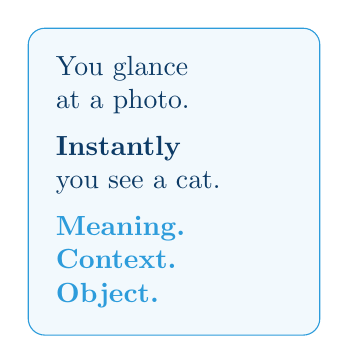
\begin{tikzpicture}
        \node[draw=PB, fill=PB!6,
              rounded corners=6pt,
              text width=3.0cm, inner sep=10pt] {
          \color{PA}
          You glance\\
          at a photo.\\[5pt]
          \textbf{Instantly}\\
          you see a cat.\\[5pt]
          {\color{PB}\bfseries
            Meaning.\\
            Context.\\
            Object.}
        };
      \end{tikzpicture}
    \end{column}

    \begin{column}{0.52\textwidth}
    \centering
      %% ── real cat image ──────────────────────────────
      
\includegraphics[width=3.6cm]{cat_human.png}\\[4pt]
      {\footnotesize\bfseries\color{PB}
        ``A Cat!''}
    \end{column}

  \end{columns}

\end{column}
\end{columns}
\end{frame}

%% ════════════════════════════════════════════════════════
%%  SLIDE 3b – WHAT A COMPUTER SEES
%% ════════════════════════════════════════════════════════
\begin{frame}{Human Vision vs Computer Vision}
\vspace{4pt}
\begin{columns}[T]

\begin{column}{0.28\textwidth}
\centering\vspace{8pt}
  \begin{tikzpicture}[
    done/.style={draw=PA!25, fill=PA!4,
                 rounded corners=4pt, minimum width=2.3cm,
                 minimum height=0.56cm, font=\footnotesize\bfseries,
                 text=PA!35, align=center},
    spot/.style={draw=red, fill=red!7, rounded corners=4pt,
                 minimum width=2.3cm, minimum height=0.56cm,
                 font=\footnotesize\bfseries, text=red,
                 align=center, line width=2pt},
    next/.style={draw=PA!20, fill=PA!3,
                 rounded corners=4pt, minimum width=2.3cm,
                 minimum height=0.56cm, font=\footnotesize\bfseries,
                 text=PA!28, align=center},
    arr/.style={->, line width=1.2pt, color=PA!20},
    sarr/.style={->, line width=1.8pt, color=red}
  ]
    \node[done] (s1) at (0, 0.00) {\faEye\; Human Sees};
    \draw[sarr] (s1.south) -- ++(0,-0.38);
    \node[spot] (s2) at (0,-1.00) {\faDesktop\; Computer Sees};
    \draw[arr]  (s2.south) -- ++(0,-0.38);
    \node[next] (s3) at (0,-2.00) {The Gap};
    \draw[arr]  (s3.south) -- ++(0,-0.38);
    \node[next] (s4) at (0,-3.00) {\faBrain\; CNN Bridges It};
  \end{tikzpicture}
\end{column}

\begin{column}{0.69\textwidth}
\vspace{4pt}
  {\color{red}\footnotesize\bfseries
    \faDesktop\; Step 2 of 4 --
    \underline{What a Computer Sees}}\\[6pt]

  \begin{columns}[T]

    \begin{column}{0.34\textwidth}
    \vspace{4pt}
      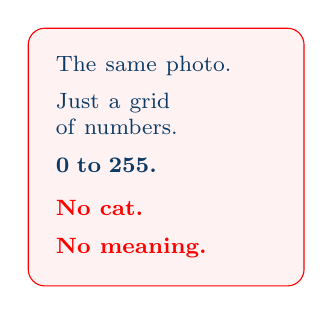
\begin{tikzpicture}
        \node[draw=red, fill=red!5,
              rounded corners=6pt,
              text width=2.8cm, inner sep=10pt] {
          \footnotesize\color{PA}
          The same photo.\\[4pt]
          Just a grid\\
          of numbers.\\[4pt]
          {\bfseries 0\;to\;255.}\\[6pt]
          {\color{red}\bfseries
            No cat.\\[2pt]
            No meaning.}
        };
      \end{tikzpicture}
    \end{column}

    \begin{column}{0.62\textwidth}
    \centering\vspace{2pt}
      %% ── real pixel grid image ───────────────────────
      
\includegraphics[width=4.2cm]{cat_computer.png}\\[4pt]
      {\fontsize{7}{7}\selectfont\bfseries\itshape
       \color{red} ``Numbers''}
    \end{column}

  \end{columns}

  \vspace{4pt}
  
\begin{tikzpicture}
    \node[draw=red!35, fill=red!4, rounded corners=4pt,
          text width=8.0cm, inner sep=5pt,
          font=\fontsize{7.5}{7.5}\selectfont\itshape
          \color{PA}, align=center] {
      {\color{red}
        same image -- to the machine,
        only a matrix of numbers.}
    };
  \end{tikzpicture}

\end{column}
\end{columns}
\end{frame}

%% ════════════════════════════════════════════════════════
%%  SLIDE 3c – THE GAP
%% ════════════════════════════════════════════════════════
\begin{frame}{Human Vision vs Computer Vision}
\vspace{4pt}
\begin{columns}[T]

\begin{column}{0.28\textwidth}
\centering\vspace{8pt}
  \begin{tikzpicture}[
    done/.style={draw=PA!25, fill=PA!4,
                 rounded corners=4pt, minimum width=2.3cm,
                 minimum height=0.56cm, font=\footnotesize\bfseries,
                 text=PA!35, align=center},
    spot/.style={draw=PD, fill=PD!8, rounded corners=4pt,
                 minimum width=2.3cm, minimum height=0.56cm,
                 font=\footnotesize\bfseries, text=PD,
                 align=center, line width=2pt},
    next/.style={draw=PA!20, fill=PA!3,
                 rounded corners=4pt, minimum width=2.3cm,
                 minimum height=0.56cm, font=\footnotesize\bfseries,
                 text=PA!28, align=center},
    arr/.style={->, line width=1.2pt, color=PA!20},
    sarr/.style={->, line width=1.8pt, color=PD}
  ]
    \node[done] (s1) at (0, 0.00) {\faEye\; Human Sees};
    \draw[arr]  (s1.south) -- ++(0,-0.38);
    \node[done] (s2) at (0,-1.00) {\faDesktop\; Computer Sees};
    \draw[sarr] (s2.south) -- ++(0,-0.38);
    \node[spot] (s3) at (0,-2.00) {The Gap};
    \draw[arr]  (s3.south) -- ++(0,-0.38);
    \node[next] (s4) at (0,-3.00) {\faBrain\; CNN Bridges It};
  \end{tikzpicture}
\end{column}

\begin{column}{0.69\textwidth}
\vspace{4pt}

  {\color{PD}\footnotesize\bfseries
    \faSearch\; Step 3 of 4 -- \underline{The Gap}}\\[8pt]

  \begin{columns}[c]

    %% ── cat image box ─────────────────────────────────
    \begin{column}{0.44\textwidth}
    \centering
      \begin{tikzpicture}
        \node[draw=PC, fill=PC!8,
              rounded corners=6pt, inner sep=6pt] {
          
\includegraphics[width=3.0cm]{cat_human.png}
        };
      \end{tikzpicture}\\[4pt]
      {\color{PC!70!black}\footnotesize\bfseries
        Sees: ``Cat''}
    \end{column}

    %% ── gap divider ───────────────────────────────────
    \begin{column}{0.08\textwidth}
    \centering\vspace{10pt}
      
\begin{tikzpicture}
        \draw[red!50, line width=1.4pt, dashed]
          (0,0) -- (0,3.80);
        \node[rotate=90,
              font=\fontsize{7}{7}\selectfont\bfseries,
              color=red] at (0,1.90) {THE GAP};
      \end{tikzpicture}
    \end{column}

    %% ── pixel grid box ────────────────────────────────
    \begin{column}{0.44\textwidth}
    \centering
      \begin{tikzpicture}
        \node[draw=red, fill=red!5,
              rounded corners=6pt, inner sep=6pt] {
          
\includegraphics[width=3.0cm]{cat_computer.png}
        };
      \end{tikzpicture}\\[4pt]
      {\color{red}\footnotesize\bfseries
        Sees: ``Numbers''}
    \end{column}

  \end{columns}

  \vspace{8pt}
  \centering
  
\begin{tikzpicture}
    \node[draw=PD, fill=PD!8,
          rounded corners=5pt,
          text width=8.2cm, inner sep=8pt,
          font=\fontsize{9}{9}\selectfont\bfseries
          , text=PD, align=center] {
      {\color{PD}How do we close this gap?}
    };
  \end{tikzpicture}

\end{column}
\end{columns}
\end{frame}

%% ════════════════════════════════════════════════════════
%%  SLIDE 3d – CNN BRIDGES THE GAP
%% ════════════════════════════════════════════════════════
\begin{frame}{Human Vision vs Computer Vision}
\vspace{2pt}
\begin{columns}[T]

\begin{column}{0.26\textwidth}
\centering\vspace{8pt}
  \begin{tikzpicture}[
    done/.style={draw=PA!25, fill=PA!4,
                 rounded corners=4pt, minimum width=2.2cm,
                 minimum height=0.54cm, font=\footnotesize\bfseries,
                 text=PA!35, align=center},
    spot/.style={draw=PB, fill=PB!8,
                 rounded corners=4pt, minimum width=2.2cm,
                 minimum height=0.54cm, font=\footnotesize\bfseries,
                 text=PB, align=center, line width=2pt},
    arr/.style={->, line width=1.2pt, color=PA!20},
    sarr/.style={->, line width=1.8pt, color=PB}
  ]
    \node[done] (s1) at (0, 0.00) {\faEye\; Human Sees};
    \draw[arr]  (s1.south) -- ++(0,-0.38);
    \node[done] (s2) at (0,-1.00) {\faDesktop\; Computer Sees};
    \draw[arr]  (s2.south) -- ++(0,-0.38);
    \node[done] (s3) at (0,-2.00) {The Gap};
    \draw[sarr] (s3.south) -- ++(0,-0.38);
    \node[spot] (s4) at (0,-3.00) {\faBrain\; CNN Bridges It};
  \end{tikzpicture}
\end{column}

\begin{column}{0.72\textwidth}
\vspace{2pt}

  {\color{PB}\footnotesize\bfseries
    \faBrain\; Step 4 of 4 --
    \underline{CNN Bridges the Gap}}\\[4pt]

  \begin{tikzpicture}

            \node[font=\fontsize{8}{8}\selectfont\bfseries,
              color=PA] at (1.28, 2.82) {Numbers in};

    %% ── pixel grid image ─────────────────────────────
    \node at (1.28, 1.28) {
      
\includegraphics[width=2.56cm]{cat_computer.png}
    };

    %% ── arrow 1 ──────────────────────────────────────
    \draw[-{Stealth[length=4mm,width=2.4mm]},
          line width=2.2pt, PB]
      (2.60,1.28) -- (3.66,1.28);
    \node[above, font=\fontsize{7}{7}\selectfont\bfseries,
          color=PB] at (3.13,1.30) {CNN};

    %% ── filter stack ─────────────────────────────────
    \foreach \k in {2,1,0}{
      \pgfmathsetmacro{\fx}{3.70+\k*0.14}
      \pgfmathsetmacro{\fy}{0.36+\k*0.12}
      \pgfmathsetmacro{\fw}{0.88-\k*0.06}
      \pgfmathsetmacro{\fh}{1.84-\k*0.24}
      \fill[PC!\the\numexpr40+\k*20\relax!white,
            opacity=0.88]
        (\fx,\fy) rectangle ++(\fw,\fh);
      \draw[PB!55,line width=0.7pt]
        (\fx,\fy) rectangle ++(\fw,\fh);
    }
    \node[below, font=\fontsize{6.5}{6.5}\selectfont\bfseries,
          color=PB] at (4.16,0.34) {filters};

    %% ── arrow 2 ──────────────────────────────────────
    \draw[-{Stealth[length=4mm,width=2.4mm]},
          line width=2.2pt, green!55!black]
      (4.64,1.28) -- (5.66,1.28);

    %% ── output cat image ─────────────────────────────
    \node at (6.80, 1.28) {
      
\includegraphics[width=2.20cm]{cat_human.png}
    };

    \node[font=\fontsize{8}{8}\selectfont\bfseries,
          color=green!55!black]
      at (6.80, 2.60) {Meaning out};

    \node[draw=green!55!black, fill=green!8,
          rounded corners=3pt, inner sep=4pt,
          font=\fontsize{7.5}{7.5}\selectfont\bfseries,
          text=green!55!black]
      at (6.80, -0.10) {Cat: 97\%};

  \end{tikzpicture}

  \vspace{4pt}
  
\begin{tikzpicture}
    \node[draw=PB, fill=PB!6,
          rounded corners=5pt,
          text width=8.8cm, inner sep=7pt,
          font=\fontsize{9}{9}\selectfont\bfseries
          , text=PA, align=center] {
      {\color{green!55!black}\faCheck}\;
      Numbers in.\quad Meaning out.\quad
      {\color{PB} That is CNN.}
    };
  \end{tikzpicture}

\end{column}
\end{columns}
\end{frame}

%% ════════════════════════════════════════════════════════
%%  SLIDE – WHAT IS A NEURAL NETWORK?
%% ════════════════════════════════════════════════════════
\begin{frame}{What is a Neural Network?}
\vspace{4pt}

\begin{columns}[T]

\begin{column}{0.30\textwidth}
\centering
\vspace{8pt}

  \begin{tikzpicture}[
    spot/.style={draw=PB, fill=PB!12,
                 rounded corners=4pt,
                 minimum width=2.4cm,
                 minimum height=0.62cm,
                 font=\footnotesize\bfseries,
                 text=PB, align=center,
                 line width=2pt},
    next/.style={draw=PA!20, fill=PA!4,
                 rounded corners=4pt,
                 minimum width=2.4cm,
                 minimum height=0.62cm,
                 font=\footnotesize\bfseries,
                 text=PA!30, align=center},
    arr/.style={->, line width=1.2pt, color=PA!20}
  ]
    \node[spot] (s1) at (0,  0.00)
      {\faBrain\; What is a NN?};
    \draw[arr] (s1.south) -- ++(0,-0.38);
    \node[next] (s2) at (0, -1.00)
      {\faTimes\; Problem 1};
    \draw[arr] (s2.south) -- ++(0,-0.38);
    \node[next] (s3) at (0, -2.00)
      {\faTimes\; Problem 2};
    \draw[arr] (s3.south) -- ++(0,-0.38);
    \node[next] (s4) at (0, -3.00)
      {\faTimes\; Problem 3};
  \end{tikzpicture}

\end{column}

\begin{column}{0.66\textwidth}
\vspace{8pt}

  {\color{PB}\footnotesize\bfseries
    \faBrain\; Before CNN --
    \underline{What is a Neural Network?}}\\[8pt]

  \begin{columns}[T]

    \begin{column}{0.46\textwidth}
      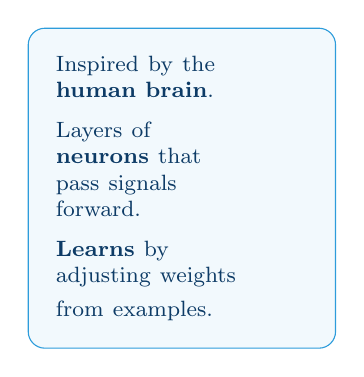
\begin{tikzpicture}
        \node[draw=PB, fill=PB!6,
              rounded corners=6pt,
              text width=3.2cm,
              inner sep=10pt] {
          \footnotesize\color{PA}
          Inspired by the\\
          \textbf{human brain}.\\[5pt]
          Layers of\\
          \textbf{neurons} that\\
          pass signals\\
          forward.\\[5pt]
          \textbf{Learns} by\\
          adjusting weights\\
          from examples.
        };
      \end{tikzpicture}
    \end{column}

    \begin{column}{0.50\textwidth}
      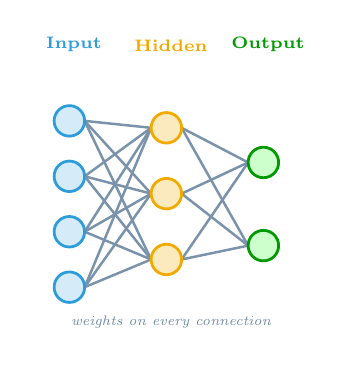
\begin{tikzpicture}[scale=0.88]

        %% ── connections FIRST (drawn behind neurons) ──

        %% input → hidden
        \foreach \i in {0,1,2,3}{
          \foreach \j in {0,1,2}{
            \draw[PA!55, line width=0.9pt]
              (0.22, \i*0.80)
              -- (1.18, \j*0.95+0.40);
          }
        }

        %% hidden → output
        \foreach \i in {0,1,2}{
          \foreach \j in {0,1}{
            \draw[PA!55, line width=0.9pt]
              (1.62, \i*0.95+0.40)
              -- (2.58, \j*1.20+0.60);
          }
        }

        %% ── neurons ON TOP of connections ─────────────

        %% input layer
        \foreach \i in {0,1,2,3}{
          \filldraw[fill=PB!20, draw=PB,
                    line width=1pt]
            (0, \i*0.80) circle (0.22);
        }
        \node[above, font=\fontsize{6.5}{6.5}
              \selectfont\bfseries, color=PB]
          at (0, 3.26) {Input};

        %% hidden layer
        \foreach \i in {0,1,2}{
          \filldraw[fill=PD!25, draw=PD,
                    line width=1pt]
            (1.40, \i*0.95+0.40) circle (0.22);
        }
        \node[above, font=\fontsize{6.5}{6.5}
              \selectfont\bfseries, color=PD]
          at (1.40, 3.26) {Hidden};

        %% output layer
        \foreach \i in {0,1}{
          \filldraw[fill=green!20, draw=green!60!black,
                    line width=1pt]
            (2.80, \i*1.20+0.60) circle (0.22);
        }
        \node[above, font=\fontsize{6.5}{6.5}
              \selectfont\bfseries, color=green!60!black]
          at (2.80, 3.26) {Output};

        %% label
        \node[below, font=\fontsize{5.5}{5.5}
              \selectfont\itshape, color=PA!60]
          at (1.40, -0.28) {weights on every connection};

      \end{tikzpicture}
    \end{column}

  \end{columns}

\end{column}
\end{columns}
\end{frame}

%% ════════════════════════════════════════════════════════
%%  SLIDE – BUT NORMAL NN STRUGGLES WITH IMAGES
%% ════════════════════════════════════════════════════════
\begin{frame}{Problems with Neural Networks}
\vspace{4pt}

\begin{columns}[T]

\begin{column}{0.30\textwidth}
\centering
\vspace{8pt}

  \begin{tikzpicture}[
    done/.style={draw=PA!30, fill=PA!5,
                 rounded corners=4pt,
                 minimum width=2.4cm,
                 minimum height=0.62cm,
                 font=\footnotesize\bfseries,
                 text=PA!40, align=center},
    spot/.style={draw=red, fill=red!8,
                 rounded corners=4pt,
                 minimum width=2.4cm,
                 minimum height=0.62cm,
                 font=\footnotesize\bfseries,
                 text=red, align=center,
                 line width=2pt},
    next/.style={draw=PA!20, fill=PA!4,
                 rounded corners=4pt,
                 minimum width=2.4cm,
                 minimum height=0.62cm,
                 font=\footnotesize\bfseries,
                 text=PA!30, align=center},
    arr/.style={->, line width=1.2pt, color=PA!20},
    sarr/.style={->, line width=1.8pt, color=red}
  ]
    \node[done] (s1) at (0,  0.00)
      {\faBrain\; What is a NN?};
    \draw[sarr] (s1.south) -- ++(0,-0.38);
    \node[spot] (s2) at (0, -1.00)
      {\faTimes\; Problem 1};
    \draw[arr] (s2.south) -- ++(0,-0.38);
    \node[next] (s3) at (0, -2.00)
      {\faTimes\; Problem 2};
    \draw[arr] (s3.south) -- ++(0,-0.38);
    \node[next] (s4) at (0, -3.00)
      {\faTimes\; Problem 3};
  \end{tikzpicture}

\end{column}

\begin{column}{0.66\textwidth}
\vspace{8pt}

  {\color{red}\footnotesize\bfseries
    \faTimes\; But --
    \underline{Normal NN Struggles with Images}}\\[8pt]

  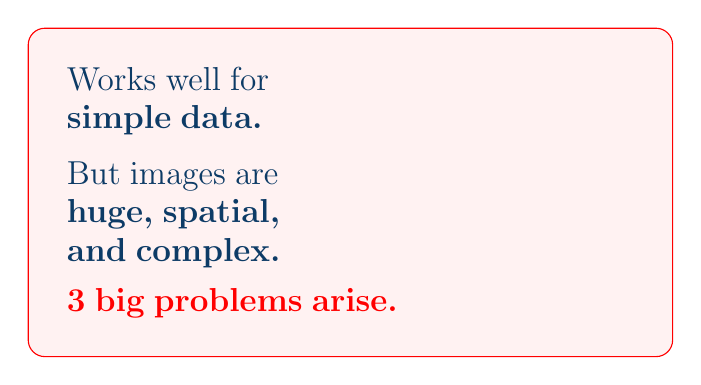
\begin{tikzpicture}
    \node[draw=red, fill=red!5,
          rounded corners=6pt,
          text width=7.2cm,
          inner sep=14pt] {
      \color{PA}
      \large
      Works well for\\
      \textbf{simple data.}\\[6pt]
      But images are\\
      \textbf{huge, spatial,\\
      and complex.}\\[6pt]
      {\color{red}\bfseries
        3 big problems arise.}
    };
  \end{tikzpicture}

\end{column}
\end{columns}
\end{frame}
%% ════════════════════════════════════════════════════════
%%  SLIDE 4a-1 – PROBLEM 1 : ONE NEURON  (clipping fixed)
%% ════════════════════════════════════════════════════════
\begin{frame}{Problem 1 -- Way Too Many Parameters}
\vspace{2pt}
\begin{columns}[T]

\begin{column}{0.30\textwidth}
\centering\vspace{8pt}
  \begin{tikzpicture}[
    spot/.style={draw=red, fill=red!8, rounded corners=4pt,
                 minimum width=2.4cm, minimum height=0.62cm,
                 font=\footnotesize\bfseries, text=red,
                 align=center, line width=2pt},
    next/.style={draw=PA!20, fill=PA!4,
                 rounded corners=4pt, minimum width=2.4cm,
                 minimum height=0.62cm, font=\footnotesize\bfseries,
                 text=PA!30, align=center},
    arr/.style={->, line width=1.2pt, color=PA!20}
  ]
    \node[spot] (p1) at (0,  0.00) {\faTimes\; Problem 1};
    \draw[arr] (p1.south) -- ++(0,-0.38);
    \node[next] (p2) at (0, -1.00) {\faTimes\; Problem 2};
    \draw[arr] (p2.south) -- ++(0,-0.38);
    \node[next] (p3) at (0, -2.00) {\faTimes\; Problem 3};
  \end{tikzpicture}
\end{column}

\begin{column}{0.66\textwidth}
\vspace{2pt}
  {\color{red}\fontsize{8.2}{8.2}\selectfont\bfseries
    \faTimes\; Problem 1 --
    \underline{Every pixel connected to every neuron}}\\[4pt]

  %% ── compact statement ────────────────────────────
  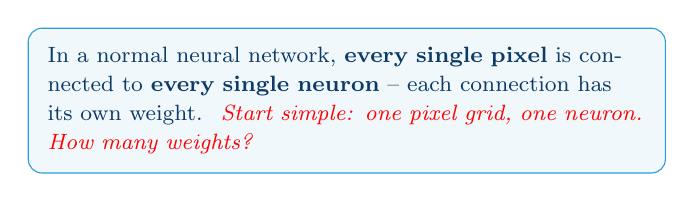
\begin{tikzpicture}
    \node[draw=PB, fill=PB!7,
          rounded corners=5pt,
        text width=7.6cm, inner sep=7pt,
          font=\fontsize{7.9}{10.4}\selectfont
          \color{PA}] {
      \raggedright
      In a normal neural network,
      \textbf{every single pixel} is connected to
      \textbf{every single neuron} --
      each connection has its own weight.\;
      {\color{red}\itshape
        Start simple: one pixel grid,
        one neuron. How many weights?}
    };
  \end{tikzpicture}

  \vspace{2pt}
  \centering

  %% ── everything in one tikzpicture ────────────────
  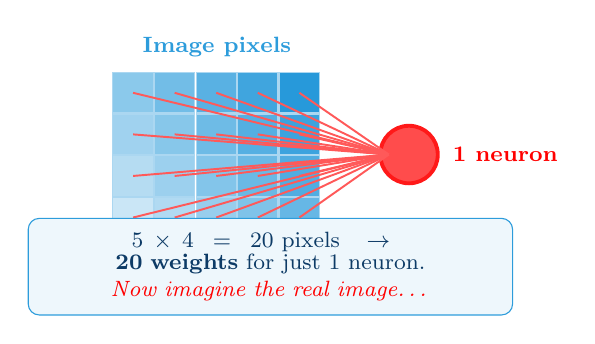
\begin{tikzpicture}[scale=0.80]

    %% label
    \node[above, font=\fontsize{8.0}{8.0}\selectfont\bfseries,
          color=PB] at (1.65, 2.72) {Image pixels};

    %% pixel grid 5×4
    \foreach \ii in {0,...,4}{
      \foreach \jj in {0,...,3}{
        \pgfmathtruncatemacro{\g}{25+\ii*12+\jj*10}
        \fill[PB!\g!white]
          (\ii*0.66,\jj*0.66) rectangle ++(0.64,0.64);
        \draw[PB!40]
          (\ii*0.66,\jj*0.66) rectangle ++(0.64,0.64);
      }
    }

    %% ONE neuron
    \filldraw[fill=red!70, draw=red!90, line width=1.4pt]
      (4.70, 1.32) circle (13pt);
    \node[right=5pt, font=\footnotesize\bfseries,
          color=red] at (5.02, 1.32) {1 neuron};

    %% edges — all pixels → 1 neuron
    \foreach \ii in {0,...,4}{
      \foreach \jj in {0,...,3}{
        \draw[red!65, line width=0.7pt]
          (\ii*0.66+0.32, \jj*0.66+0.32)
          -- (4.38, 1.32);
      }
    }

    %% weight count badge
    \node[draw=PB, fill=PB!8,
          rounded corners=4pt, inner sep=5pt,
          text width=5.8cm, align=center,
          font=\fontsize{7.9}{7.9}\selectfont
          \color{PA}]
      at (2.50, -0.46) {
        $5 \times 4 = 20$ pixels
        $\;\to\;$ \textbf{20 weights}
        for just 1 neuron.\\[2pt]
        {\color{red}\itshape
          Now imagine the real image\ldots}
      };

  \end{tikzpicture}

\end{column}
\end{columns}
\end{frame}

%% ════════════════════════════════════════════════════════
%%  SLIDE 4a-2 – PROBLEM 1 : FULL LAYER EXPLOSION
%% ════════════════════════════════════════════════════════
\begin{frame}{Problem 1 -- Way Too Many Parameters}
\vspace{1pt}
\begin{columns}[T]

\begin{column}{0.30\textwidth}
\centering\vspace{4pt}
  \begin{tikzpicture}[
    spot/.style={draw=red, fill=red!8, rounded corners=4pt,
                 minimum width=2.4cm, minimum height=0.62cm,
                 font=\footnotesize\bfseries, text=red,
                 align=center, line width=2pt},
    next/.style={draw=PA!20, fill=PA!4,
                 rounded corners=4pt, minimum width=2.4cm,
                 minimum height=0.62cm, font=\footnotesize\bfseries,
                 text=PA!30, align=center},
    arr/.style={->, line width=1.2pt, color=PA!20}
  ]
    \node[spot] (p1) at (0,  0.00) {\faTimes\; Problem 1};
    \draw[arr] (p1.south) -- ++(0,-0.38);
    \node[next] (p2) at (0, -1.00) {\faTimes\; Problem 2};
    \draw[arr] (p2.south) -- ++(0,-0.38);
    \node[next] (p3) at (0, -2.00) {\faTimes\; Problem 3};
  \end{tikzpicture}
\end{column}

\begin{column}{0.66\textwidth}
\vspace{4pt}
  {\color{red}\footnotesize\bfseries
    \faTimes\; Problem 1 --
    \underline{Every pixel to EVERY neuron}}\\[8pt]

  \centering
  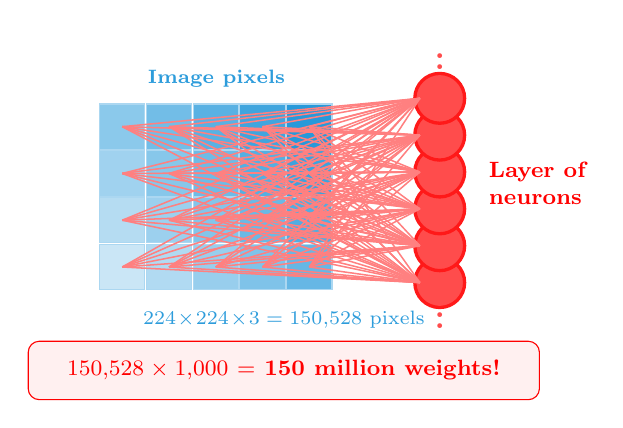
\begin{tikzpicture}[scale=0.90]

    %% ── pixel grid 5×4 ───────────────────────────────
    \foreach \ii in {0,...,4}{
      \foreach \jj in {0,...,3}{
        \pgfmathtruncatemacro{\g}{25+\ii*12+\jj*10}
        \fill[PB!\g!white]
          (\ii*0.66,\jj*0.66) rectangle ++(0.64,0.64);
        \draw[PB!40]
          (\ii*0.66,\jj*0.66) rectangle ++(0.64,0.64);
      }
    }
    \node[above, font=\fontsize{7.5}{7.5}\selectfont\bfseries,
          color=PB] at (1.65,2.72) {Image pixels};

    %% ── 6 neurons ────────────────────────────────────
    \foreach \nn in {0,...,5}{
      \filldraw[fill=red!70, draw=red!90, line width=1.2pt]
        (4.80, \nn*0.52+0.10) circle (10pt);
    }
    \node[right=6pt, font=\footnotesize\bfseries,
          color=red, align=left]
      at (5.12,1.50) {Layer of\\neurons};

    %% dots to imply more neurons
    \node[font=\large\bfseries, color=red!70]
      at (4.80,-0.24) {$\vdots$};
    \node[font=\large\bfseries, color=red!70]
      at (4.80, 3.26) {$\vdots$};

    %% ── every pixel → every neuron (darkened) ────────
    \foreach \ii in {0,...,4}{
      \foreach \jj in {0,...,3}{
        \foreach \nn in {0,...,5}{
          \draw[red!50, line width=0.55pt]
            (\ii*0.66+0.32, \jj*0.66+0.32)
            -- (4.52, \nn*0.52+0.10);
        }
      }
    }

    %% ── pixel count ──────────────────────────────────
    \node[font=\fontsize{7}{7}\selectfont,
          color=PB] at (2.60,-0.42)
      {$224\!\times\!224\!\times\!3
        = 150{,}528$ pixels};

    %% ── explosion badge ──────────────────────────────
    \node[draw=red, fill=red!6,
          rounded corners=4pt, inner sep=7pt,
          text width=6.0cm, align=center,
          font=\fontsize{8.5}{8.5}\selectfont
          \bfseries\color{red}]
      at (2.60,-1.14)
      {$150{,}528 \times 1{,}000
        = \textbf{150 million weights!}$};

  \end{tikzpicture}

\end{column}
\end{columns}
\end{frame}

%% ════════════════════════════════════════════════════════
%%  SLIDE 4a-3 – PROBLEM 1 : EXPLANATION
%% ════════════════════════════════════════════════════════
\begin{frame}{Problem 1 -- Way Too Many Parameters}
\vspace{4pt}
\begin{columns}[T]

\begin{column}{0.30\textwidth}
\centering\vspace{8pt}
  \begin{tikzpicture}[
    spot/.style={draw=red, fill=red!8, rounded corners=4pt,
                 minimum width=2.4cm, minimum height=0.62cm,
                 font=\footnotesize\bfseries, text=red,
                 align=center, line width=2pt},
    next/.style={draw=PA!20, fill=PA!4,
                 rounded corners=4pt, minimum width=2.4cm,
                 minimum height=0.62cm, font=\footnotesize\bfseries,
                 text=PA!30, align=center},
    arr/.style={->, line width=1.2pt, color=PA!20}
  ]
    \node[spot] (p1) at (0,  0.00) {\faTimes\; Problem 1};
    \draw[arr] (p1.south) -- ++(0,-0.38);
    \node[next] (p2) at (0, -1.00) {\faTimes\; Problem 2};
    \draw[arr] (p2.south) -- ++(0,-0.38);
    \node[next] (p3) at (0, -2.00) {\faTimes\; Problem 3};
  \end{tikzpicture}
\end{column}

\begin{column}{0.66\textwidth}
\vspace{2pt}
  {\color{red}\footnotesize\bfseries
    \faTimes\; Problem 1 --
    \underline{Why This Breaks Everything}}\\[6pt]

  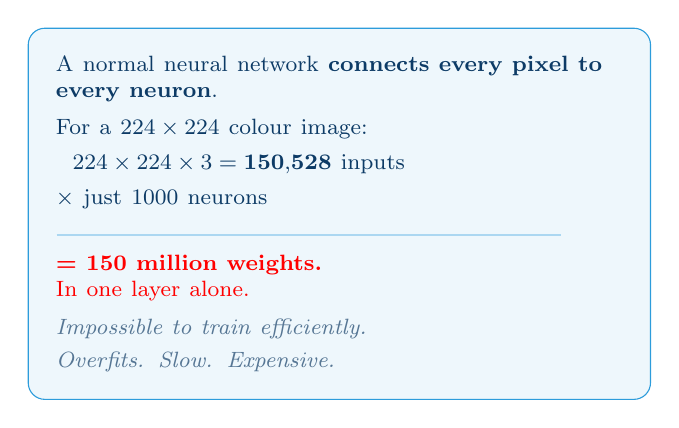
\begin{tikzpicture}
    \node[draw=PB, fill=PB!8,
          rounded corners=6pt,
          text width=7.2cm, inner sep=10pt] {
      \footnotesize\color{PA}
      A normal neural network
      \textbf{connects every pixel to
      every neuron}.\\[4pt]
      For a $224\times224$ colour image:\\[3pt]
      \hspace{6pt}$224 \times 224 \times 3
        = \mathbf{150{,}528}$ inputs\\[3pt]
      $\times$ just 1000 neurons\\[2pt]
      \tikz\draw[PB!40, line width=0.6pt]
        (0,0)--(6.4cm,0);\\[3pt]
      {\color{red}\bfseries
        = 150 million weights.}\\
      {\color{red} In one layer alone.}\\[4pt]
      \footnotesize\itshape\color{PA!70}
      Impossible to train efficiently.\\
      Overfits. Slow. Expensive.
    };
  \end{tikzpicture}

\end{column}
\end{columns}
\end{frame}
%% ════════════════════════════════════════════════════════
%%  SLIDE 4b-1 – PROBLEM 2 : VISUAL  (full rework)
%% ════════════════════════════════════════════════════════
\begin{frame}{Problem 2 -- Spatial Structure is Destroyed}
\vspace{2pt}
\begin{columns}[T]

\begin{column}{0.30\textwidth}
\centering\vspace{8pt}
  \begin{tikzpicture}[
    done/.style={draw=PA!30, fill=PA!5,
                 rounded corners=4pt, minimum width=2.4cm,
                 minimum height=0.62cm, font=\footnotesize\bfseries,
                 text=PA!40, align=center},
    spot/.style={draw=red, fill=red!8, rounded corners=4pt,
                 minimum width=2.4cm, minimum height=0.62cm,
                 font=\footnotesize\bfseries, text=red,
                 align=center, line width=2pt},
    next/.style={draw=PA!20, fill=PA!4,
                 rounded corners=4pt, minimum width=2.4cm,
                 minimum height=0.62cm, font=\footnotesize\bfseries,
                 text=PA!30, align=center},
    arr/.style={->, line width=1.2pt, color=PA!20}
  ]
    \node[done] (p1) at (0,  0.00) {\faTimes\; Problem 1};
    \draw[arr] (p1.south) -- ++(0,-0.38);
    \node[spot] (p2) at (0, -1.00) {\faTimes\; Problem 2};
    \draw[arr] (p2.south) -- ++(0,-0.38);
    \node[next] (p3) at (0, -2.00) {\faTimes\; Problem 3};
  \end{tikzpicture}
\end{column}

\begin{column}{0.66\textwidth}
\vspace{2pt}
  {\color{red}\footnotesize\bfseries
    \faTimes\; Problem 2 --
    \underline{What Flattening Does}}\\[5pt]

  %% ── top row: 2D grid | arrow | 1D strip ──────────────
  \begin{columns}[T]

    %% LEFT: 2D grid
    \begin{column}{0.40\textwidth}
      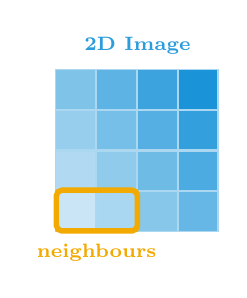
\begin{tikzpicture}[scale=0.72]
        \node[above, font=\fontsize{7.5}{7.5}\selectfont\bfseries,
              color=PB] at (1.44,2.96) {2D Image};
        \foreach \ii in {0,...,3}{
          \foreach \jj in {0,...,3}{
            \pgfmathtruncatemacro{\g}{25+\ii*16+\jj*12}
            \fill[PB!\g!white]
              (\ii*0.72, \jj*0.72) rectangle ++(0.70,0.70);
            \draw[PB!40]
              (\ii*0.72, \jj*0.72) rectangle ++(0.70,0.70);
          }
        }
        %% PD neighbour box
        \draw[PD, line width=2pt, rounded corners=2pt]
          (0.01, 0.01) rectangle ++(1.43,0.72);
        %% neighbour label BELOW grid -- plenty of space
        \node[below, font=\fontsize{7}{7}\selectfont\bfseries,
              color=PD]
          at (0.72, -0.04) {neighbours};
      \end{tikzpicture}
    \end{column}

    %% MIDDLE: arrow
    \begin{column}{0.12\textwidth}
      \vspace{20pt}
      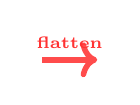
\begin{tikzpicture}
        \draw[->, line width=2pt, red!70]
          (0,0) -- (0.70,0);
        \node[above, font=\fontsize{6}{6}\selectfont\bfseries,
              color=red!80] at (0.35,0.02) {flatten};
      \end{tikzpicture}
    \end{column}

    %% RIGHT: 1D strip + X label
    \begin{column}{0.44\textwidth}
      \vspace{14pt}
      \begin{tikzpicture}[scale=0.72]
        %% 1D strip
        \foreach \kk in {0,...,4}{
          \pgfmathtruncatemacro{\g}{25+\kk*14}
          \fill[PB!\g!white]
            (\kk*0.50, 0.50) rectangle ++(0.48,0.48);
          \draw[PB!45]
            (\kk*0.50, 0.50) rectangle ++(0.48,0.48);
        }
        \node[right, font=\fontsize{7}{7}\selectfont,
              color=PA] at (2.52,0.74) {$\cdots$};
        \node[above, font=\fontsize{7}{7}\selectfont\itshape,
              color=PA] at (1.24,1.00) {1D list};
        %% X label below strip
        \node[below, font=\fontsize{8}{8}\selectfont\bfseries,
              color=red] at (1.24,0.48)
          {\faTimes\ \fontsize{7}{7}\selectfont
           neighbours gone};
      \end{tikzpicture}
    \end{column}

  \end{columns}

  \vspace{6pt}

  %% ── description box ──────────────────────────────────
  
\begin{tikzpicture}
    \node[draw=red, fill=red!5, rounded corners=5pt,
          text width=7.2cm, inner sep=8pt,
          font=\footnotesize\color{PA}, align=center] {
      All spatial relationships vanish.\\
      No idea which pixels were neighbours.
    };
  \end{tikzpicture}

\end{column}
\end{columns}
\end{frame}

%% ════════════════════════════════════════════════════════
%%  SLIDE 4b-2 – PROBLEM 2 : ANALOGY  (full rework)
%% ════════════════════════════════════════════════════════
\begin{frame}{Problem 2 -- Spatial Structure is Destroyed}
\vspace{2pt}
\begin{columns}[T]

\begin{column}{0.30\textwidth}
\centering\vspace{8pt}
  \begin{tikzpicture}[
    done/.style={draw=PA!30, fill=PA!5,
                 rounded corners=4pt, minimum width=2.4cm,
                 minimum height=0.62cm, font=\footnotesize\bfseries,
                 text=PA!40, align=center},
    spot/.style={draw=red, fill=red!8, rounded corners=4pt,
                 minimum width=2.4cm, minimum height=0.62cm,
                 font=\footnotesize\bfseries, text=red,
                 align=center, line width=2pt},
    next/.style={draw=PA!20, fill=PA!4,
                 rounded corners=4pt, minimum width=2.4cm,
                 minimum height=0.62cm, font=\footnotesize\bfseries,
                 text=PA!30, align=center},
    arr/.style={->, line width=1.2pt, color=PA!20}
  ]
    \node[done] (p1) at (0,  0.00) {\faTimes\; Problem 1};
    \draw[arr] (p1.south) -- ++(0,-0.38);
    \node[spot] (p2) at (0, -1.00) {\faTimes\; Problem 2};
    \draw[arr] (p2.south) -- ++(0,-0.38);
    \node[next] (p3) at (0, -2.00) {\faTimes\; Problem 3};
  \end{tikzpicture}
\end{column}

\begin{column}{0.66\textwidth}
\vspace{2pt}
  {\color{PD}\footnotesize\bfseries
    \faPuzzlePiece\; Real-Life Analogy}\\[6pt]

  \begin{columns}[T]

    %% LEFT: assembled puzzle
    \begin{column}{0.38\textwidth}
      \centering
      {\color{PB}\fontsize{7.5}{7.5}\selectfont\bfseries
        Assembled Puzzle}\\[4pt]
      \begin{tikzpicture}[scale=0.72]
        \fill[PA!6, rounded corners=3pt]
          (-0.04,-0.04) rectangle (2.92,2.92);

        %% 4x4 board
        \foreach \ii in {0,...,3}{
          \foreach \jj in {0,...,3}{
            \fill[PC, rounded corners=2pt]
              (\ii*0.72+0.04, \jj*0.72+0.04)
              rectangle ++(0.66,0.66);
            \draw[white, line width=1.0pt]
              (\ii*0.72, \jj*0.72)
              rectangle ++(0.72,0.72);
          }
        }

        %% clear house shape
        \foreach \ii/\jj in {
          1/0,2/0,
          1/1,2/1,
          1/2,2/2,
          0/2,3/2,
          1/3,2/3}{
          \fill[PD!88!red, rounded corners=2pt]
            (\ii*0.72+0.04, \jj*0.72+0.04)
            rectangle ++(0.66,0.66);
          \draw[white, line width=1.0pt]
            (\ii*0.72, \jj*0.72)
            rectangle ++(0.72,0.72);
        }
      \end{tikzpicture}\\[4pt]
      {\color{green!60!black}\fontsize{7.5}{7.5}
       \selectfont\bfseries \faCheck\ clear shape}
    \end{column}

    %% MIDDLE: arrow
    \begin{column}{0.10\textwidth}
      \vspace{28pt}
      \begin{tikzpicture}
        \draw[->, line width=2pt, red!70]
          (0,0) -- (0.60,0);
        \node[above, font=\fontsize{6}{6}\selectfont\bfseries,
              color=red] at (0.30,0.02) {flatten};
      \end{tikzpicture}
    \end{column}

    %% RIGHT: horizontal random list
    \begin{column}{0.48\textwidth}
      \centering
      {\color{red}\fontsize{7.5}{7.5}\selectfont\bfseries
        Random Pile}\\[4pt]
      \begin{tikzpicture}[scale=0.72]
        \node[draw=red!45, fill=red!3,
              rounded corners=4pt,
              minimum width=3.75cm,
              minimum height=1.08cm] at (1.88,0.55) {};

        %% horizontal list of shuffled parts
        \foreach \x/\rot/\lbl in {
          0.26/12/A,
          0.98/-10/C,
          1.70/16/F,
          2.42/-14/B,
          3.14/8/E}{
          \fill[PC, rounded corners=2pt]
            (\x,0.28) rectangle ++(0.58,0.54);
          \draw[white, line width=0.9pt]
            (\x,0.28) rectangle ++(0.58,0.54);

          \fill[PD!88!red, rounded corners=2pt,
                rotate around={\rot:(\x+0.29,0.55)}]
            (\x+0.11,0.37) rectangle ++(0.36,0.36);
          \draw[white, line width=0.8pt,
                rotate around={\rot:(\x+0.29,0.55)}]
            (\x+0.11,0.37) rectangle ++(0.36,0.36);

          \node[below, font=\fontsize{6.5}{6.5}\selectfont\bfseries,
                color=PA] at (\x+0.29,0.22) {\lbl};
        }
      \end{tikzpicture}\\[4pt]
      {\color{red}\fontsize{7.5}{7.5}\selectfont\bfseries
        \faTimes\ same parts, wrong order}
    \end{column}

  \end{columns}

  \vspace{6pt}

  %% takeaway
  \begin{tikzpicture}
    \node[draw=PD, fill=PD!8, rounded corners=5pt,
          text width=7.2cm, inner sep=8pt,
          font=\footnotesize\color{PA}, align=center] {
      {\color{PD}\bfseries
        That is exactly what flattening does.}
    };
  \end{tikzpicture}

\end{column}
\end{columns}
\end{frame}
%% ════════════════════════════════════════════════════════
%%  SLIDE 4c-1 – PROBLEM 3 : VISUAL ONLY (fixed)
%% ════════════════════════════════════════════════════════
\begin{frame}{Problem 3 -- No Translation Invariance}
\vspace{0pt}
\begin{columns}[T]

\begin{column}{0.30\textwidth}
\centering\vspace{4pt}
  \begin{tikzpicture}[
    done/.style={draw=PA!30, fill=PA!5,
                 rounded corners=4pt, minimum width=2.4cm,
                 minimum height=0.62cm, font=\footnotesize\bfseries,
                 text=PA!40, align=center},
    spot/.style={draw=red, fill=red!8, rounded corners=4pt,
                 minimum width=2.4cm, minimum height=0.62cm,
                 font=\footnotesize\bfseries, text=red,
                 align=center, line width=2pt},
    arr/.style={->, line width=1.2pt, color=PA!20}
  ]
    \node[done] (p1) at (0,  0.00) {\faTimes\; Problem 1};
    \draw[arr] (p1.south) -- ++(0,-0.38);
    \node[done] (p2) at (0, -1.00) {\faTimes\; Problem 2};
    \draw[arr] (p2.south) -- ++(0,-0.38);
    \node[spot] (p3) at (0, -2.00) {\faTimes\; Problem 3};
  \end{tikzpicture}
\end{column}

\begin{column}{0.66\textwidth}
\vspace{2pt}

  {\color{red}\fontsize{8.2}{8.2}\selectfont\bfseries
    \faTimes\; Problem 3 --
    \underline{Object Moves -- Network Fails}}\\[4pt]

  \begin{columns}[T]

    %% ── LEFT grid ────────────────────────────────────────
    \begin{column}{0.42\textwidth}
    \centering
      {\fontsize{8.0}{8.0}\selectfont\bfseries\color{PB}
        Position A}\\[4pt]
      \begin{tikzpicture}[scale=0.72]
        \foreach \ii in {0,...,3}{
          \foreach \jj in {0,...,3}{
            \fill[PB!15!white]
              (\ii*0.78,\jj*0.78) rectangle ++(0.76,0.76);
            \draw[PB!35]
              (\ii*0.78,\jj*0.78) rectangle ++(0.76,0.76);
          }
        }
        \node[font=\large, color=PA]
          at (0.39, 2.73) {\faCat};
        \draw[PB, line width=2pt, rounded corners=2pt]
          (0.01,2.36) rectangle ++(0.77,0.77);
      \end{tikzpicture}\\[4pt]
      {\fontsize{8.0}{8.0}\selectfont\bfseries\color{green!60!black}
        \faCheck\ recognises}
    \end{column}

    %% ── ARROW ────────────────────────────────────────────
    \begin{column}{0.12\textwidth}
    \centering\vspace{18pt}
      \begin{tikzpicture}
        \draw[->, line width=2.2pt, PD]
          (0,0) -- (0.68,0);
        \node[above, font=\fontsize{6.5}{6.5}
              \selectfont\bfseries, color=PD]
          at (0.34,0.02) {move};
      \end{tikzpicture}
    \end{column}

    %% ── RIGHT grid ───────────────────────────────────────
    \begin{column}{0.42\textwidth}
    \centering
      {\fontsize{8.0}{8.0}\selectfont\bfseries\color{PB}
        Position B}\\[4pt]
      \begin{tikzpicture}[scale=0.72]
        \foreach \ii in {0,...,3}{
          \foreach \jj in {0,...,3}{
            \fill[PB!15!white]
              (\ii*0.78,\jj*0.78) rectangle ++(0.76,0.76);
            \draw[PB!35]
              (\ii*0.78,\jj*0.78) rectangle ++(0.76,0.76);
          }
        }
        \node[font=\large, color=PA]
          at (2.73, 0.39) {\faCat};
        \draw[red, line width=2pt,
              rounded corners=2pt, dashed]
          (0.01,2.36) rectangle ++(0.77,0.77);
        \node[above, font=\fontsize{6.4}{6.4}
              \selectfont\itshape, color=red]
          at (0.39, 3.14) {still looks here};
      \end{tikzpicture}\\[4pt]
      {\fontsize{8.0}{8.0}\selectfont\bfseries\color{red}
        \faTimes\ confused}
    \end{column}

  \end{columns}

  \vspace{2pt}

  %% ── description box ──────────────────────────────────
  \begin{tikzpicture}
    \node[draw=PB, fill=PB!6,
          rounded corners=5pt,
          text width=7.2cm, inner sep=5pt,
          font=\fontsize{7.8}{9.4}\selectfont\color{PA},
          align=left] {
      The cat shifted position --
      the network \textbf{still looks at the old spot}.\\[1pt]
      It must \textbf{relearn from scratch}
      that the same cat exists at every new position.\\[1pt]
      {\color{red}\bfseries
        \faTimes\; Every shift
        = a brand new learning problem.}
    };
  \end{tikzpicture}

\end{column}
\end{columns}
\end{frame}

%% ════════════════════════════════════════════════════════
%%  SLIDE 4c-2 – PROBLEM 3 : ANALOGY  (final fix)
%% ════════════════════════════════════════════════════════
\begin{frame}{Problem 3 -- No Translation Invariance}
\vspace{2pt}
\begin{columns}[T]

\begin{column}{0.30\textwidth}
\centering\vspace{8pt}
  \begin{tikzpicture}[
    done/.style={draw=PA!30, fill=PA!5,
                 rounded corners=4pt, minimum width=2.4cm,
                 minimum height=0.62cm, font=\footnotesize\bfseries,
                 text=PA!40, align=center},
    spot/.style={draw=red, fill=red!8, rounded corners=4pt,
                 minimum width=2.4cm, minimum height=0.62cm,
                 font=\footnotesize\bfseries, text=red,
                 align=center, line width=2pt},
    arr/.style={->, line width=1.2pt, color=PA!20}
  ]
    \node[done] (p1) at (0,  0.00) {\faTimes\; Problem 1};
    \draw[arr] (p1.south) -- ++(0,-0.38);
    \node[done] (p2) at (0, -1.00) {\faTimes\; Problem 2};
    \draw[arr] (p2.south) -- ++(0,-0.38);
    \node[spot] (p3) at (0, -2.00) {\faTimes\; Problem 3};
  \end{tikzpicture}
\end{column}

%% ── RIGHT: analogy content ───────────────────────────────
\begin{column}{0.66\textwidth}
\vspace{2pt}

  {\color{PD}\footnotesize\bfseries
    \faUser\; Real-Life Analogy}\\[6pt]

  %% ── three sub-columns: left card | arrow | right card ──
  \begin{columns}[T]

    %% LEFT CARD
    \begin{column}{0.40\textwidth}
    \centering
      \begin{tikzpicture}[scale=0.80]
        %% card
        \fill[PB!12, rounded corners=5pt]
          (-1.20, -1.10) rectangle (1.20, 1.80);
        \draw[PB, line width=1.5pt, rounded corners=5pt]
          (-1.20, -1.10) rectangle (1.20, 1.80);
        %% head
        \filldraw[fill=PB!50, draw=PB,
                  line width=1pt]
          (0, 1.38) circle (0.28);
        %% torso
        \fill[PB!55]
          (-0.18, 0.82) rectangle ++(0.36,0.48);
        %% arms
        \draw[PB, line width=1.6pt, line cap=round]
          (-0.18, 1.08) -- (-0.55, 0.68);
        \draw[PB, line width=1.6pt, line cap=round]
          ( 0.18, 1.08) -- ( 0.55, 0.68);
        %% legs
        \draw[PB, line width=1.6pt, line cap=round]
          (-0.10, 0.82) -- (-0.26, 0.18);
        \draw[PB, line width=1.6pt, line cap=round]
          ( 0.10, 0.82) -- ( 0.26, 0.18);
        %% label inside
        \node[font=\fontsize{7}{7}\selectfont\itshape,
              color=PB] at (0, -0.58) {at centre};
      \end{tikzpicture}\\[4pt]
      {\footnotesize\bfseries\color{green!60!black}
        \faCheck\ recognised}
    \end{column}

    %% ARROW
    \begin{column}{0.14\textwidth}
    \centering\vspace{22pt}
      \begin{tikzpicture}
        \draw[->, line width=2.2pt, PD]
          (0,0) -- (0.72,0);
        \node[above, font=\fontsize{6.5}{6.5}
              \selectfont\bfseries, color=PD]
          at (0.36,0.02) {moves};
      \end{tikzpicture}
    \end{column}

    %% RIGHT CARD
    \begin{column}{0.40\textwidth}
    \centering
      \begin{tikzpicture}[scale=0.80]
        %% card
        \fill[red!8, rounded corners=5pt]
          (-1.20, -1.10) rectangle (1.20, 1.80);
        \draw[red, line width=1.5pt, rounded corners=5pt]
          (-1.20, -1.10) rectangle (1.20, 1.80);
        %% person shifted right
        \filldraw[fill=PB!50, draw=PB,
                  line width=1pt]
          (0.42, 1.38) circle (0.28);
        \fill[PB!55]
          (0.24, 0.82) rectangle ++(0.36,0.48);
        \draw[PB, line width=1.6pt, line cap=round]
          (0.24, 1.08) -- (-0.13, 0.68);
        \draw[PB, line width=1.6pt, line cap=round]
          (0.60, 1.08) -- ( 0.97, 0.68);
        \draw[PB, line width=1.6pt, line cap=round]
          (0.32, 0.82) -- ( 0.12, 0.18);
        \draw[PB, line width=1.6pt, line cap=round]
          (0.52, 0.82) -- ( 0.72, 0.18);
        %% ? clear of person
        \node[font=\fontsize{28}{28}\selectfont\bfseries,
              color=red!55] at (-0.56, 0.90) {?};
        %% label inside
        \node[font=\fontsize{7}{7}\selectfont\itshape,
              color=red] at (0.10, -0.58) {stepped away};
      \end{tikzpicture}\\[4pt]
      {\footnotesize\bfseries\color{red}
        \faTimes\ who is that?}
    \end{column}

  \end{columns}

  \vspace{8pt}

  %% takeaway — plain tikzpicture, after all columns
  \begin{tikzpicture}
    \node[draw=PD, fill=PD!8,
          rounded corners=5pt,
          text width=7.4cm, inner sep=8pt,
          font=\footnotesize\color{PA},
          align=center] {
      {\color{PD}\bfseries
        A normal NN knows the person\\
        only when he stands in the exact same spot.}
    };
  \end{tikzpicture}

\end{column}
\end{columns}
\end{frame}

%% ════════════════════════════════════════════════════════
%%  SLIDE 5a – CNN SOLUTION 1 : LOCAL CONNECTIVITY
%% ════════════════════════════════════════════════════════
\begin{frame}{How CNN Solves All Three Problems}
\vspace{8pt}

\centering
\begin{tikzpicture}[
  prob/.style={draw=red!40, fill=red!5,
               rounded corners=5pt,
               text width=3.0cm,
               minimum height=0.90cm,
               inner sep=8pt,
               font=\footnotesize\color{PA!50},
               align=left},
  probspot/.style={draw=red!80, fill=red!8,
               rounded corners=5pt,
               text width=3.0cm,
               minimum height=0.90cm,
               inner sep=8pt,
               font=\footnotesize\color{PA},
               align=left},
  garr/.style={->, line width=2pt, color=PA!20},
  sarr/.style={->, line width=2.5pt, color=PD}
]

  %% ── Row 1 ACTIVE ──────────────────────────────────────
  \node[probspot] (p1) at (0, 0) {
    {\color{red}\bfseries 1.}\; Parameter\\explosion
  };
  \draw[sarr] ($(p1.east)+(0.12,0)$) -- ++(0.55,0);
  \node[anchor=west,
        font=\footnotesize\color{PB}, align=left,
        draw=PB, fill=PB!3,
        rounded corners=5pt, text width=6.2cm,
        minimum height=0.90cm, inner sep=10pt]
    at ($(p1.east)+(0.78,0)$) {
    {\color{PB}\bfseries Local Connectivity}\\[3pt]
    Each neuron sees only a \textbf{small patch}.\\
    Millions of weights $\to$ just hundreds.
  };

  %% ── Row 2 greyed ──────────────────────────────────────
  \node[prob, below=0.70cm of p1] (p2) {
    {\color{red!40}\bfseries 2.}\; Spatial structure lost
  };
  \draw[garr] ($(p2.east)+(0.12,0)$) -- ++(0.55,0);
  \node[anchor=west,
        font=\footnotesize\color{PA!35}, align=left,
        draw=PA!15, fill=PA!3,
        rounded corners=5pt, text width=6.2cm,
        minimum height=0.90cm, inner sep=10pt]
    at ($(p2.east)+(0.78,0)$) {
    {\color{PA!35}\bfseries Shared Weights}\\[3pt]
    The same filter slides across the image\\
    -- spatial layout preserved, weights reused.
  };

  %% ── Row 3 greyed ──────────────────────────────────────
  \node[prob, below=0.70cm of p2] (p3) {
    {\color{red!40}\bfseries 3.}\; No translation invariance
  };
  \draw[garr] ($(p3.east)+(0.12,0)$) -- ++(0.55,0);
  \node[anchor=west,
        font=\footnotesize\color{PA!35}, align=left,
        draw=PA!15, fill=PA!3,
        rounded corners=5pt, text width=6.2cm,
        minimum height=0.90cm, inner sep=10pt]
    at ($(p3.east)+(0.78,0)$) {
    {\color{PA!35}\bfseries Pooling}\\[3pt]
    Summarises local regions -- network becomes\\
    robust to shifts in object position.
  };

  %% ── Headers ───────────────────────────────────────────
  \node[above=0.28cm of p1,
        font=\footnotesize\bfseries, color=red,
        anchor=west] at (p1.north west)
    {\faTimes\; What went wrong};
  \node[above=0.28cm of p1,
        font=\footnotesize\bfseries, color=green!60!black,
        anchor=west] at ($(p1.north east)+(0.78,0.28)$)
    {\faCheck\; How CNN fixes it};

\end{tikzpicture}
\end{frame}

%% ════════════════════════════════════════════════════════
%%  SLIDE 5b – CNN SOLUTION 2 : SHARED WEIGHTS
%% ════════════════════════════════════════════════════════
\begin{frame}{How CNN Solves All Three Problems}
\vspace{8pt}

\centering
\begin{tikzpicture}[
  prob/.style={draw=red!40, fill=red!5,
               rounded corners=5pt,
               text width=3.0cm,
               minimum height=0.90cm,
               inner sep=8pt,
               font=\footnotesize\color{PA!50},
               align=left},
  probdone/.style={draw=green!50!black!40,
               fill=green!5,
               rounded corners=5pt,
               text width=3.0cm,
               minimum height=0.90cm,
               inner sep=8pt,
               font=\footnotesize\color{PA!50},
               align=left},
  probspot/.style={draw=red!80, fill=red!8,
               rounded corners=5pt,
               text width=3.0cm,
               minimum height=0.90cm,
               inner sep=8pt,
               font=\footnotesize\color{PA},
               align=left},
  garr/.style={->, line width=2pt, color=PA!20},
  sarr/.style={->, line width=2.5pt, color=PD},
  darr/.style={->, line width=2pt, color=green!50!black!40}
]

  %% ── Row 1 done ────────────────────────────────────────
  \node[probdone] (p1) at (0, 0) {
    {\color{green!60!black!60}\bfseries 1.}
    \; Parameter explosion
  };
  \draw[darr] ($(p1.east)+(0.12,0)$) -- ++(0.55,0);
  \node[anchor=west,
        font=\footnotesize\color{PA!40}, align=left,
        draw=PA!15, fill=green!3,
        rounded corners=5pt, text width=6.2cm,
        minimum height=0.90cm, inner sep=10pt]
    at ($(p1.east)+(0.78,0)$) {
    {\color{PA!40}\bfseries
      \faCheck\ Local Connectivity}\\[3pt]
    Each neuron sees only a small patch.\\
    Millions of weights $\to$ just hundreds.
  };

  %% ── Row 2 ACTIVE ──────────────────────────────────────
  \node[probspot, below=0.70cm of p1] (p2) {
    {\color{red}\bfseries 2.}\; Spatial structure lost
  };
  \draw[sarr] ($(p2.east)+(0.12,0)$) -- ++(0.55,0);
  \node[anchor=west, font=\footnotesize\color{PD}, align=left,
        draw=PD, fill=PD!3, rounded corners=5pt,
        text width=6.2cm, minimum height=0.90cm, inner sep=10pt]
    at ($(p2.east)+(0.78,0)$) {
    {\color{PD}\bfseries Shared Weights}\\[3pt]
    The \textbf{same filter} slides across the image\\
    -- spatial layout preserved, weights reused.
  };

  %% ── Row 3 greyed ──────────────────────────────────────
  \node[prob, below=0.70cm of p2] (p3) {
    {\color{red!40}\bfseries 3.}\; No translation invariance
  };
  \draw[garr] ($(p3.east)+(0.12,0)$) -- ++(0.55,0);
  \node[anchor=west,
        font=\footnotesize\color{PA!35}, align=left,
        draw=PA!15, fill=PA!3,
        rounded corners=5pt, text width=6.2cm,
        minimum height=0.90cm, inner sep=10pt]
    at ($(p3.east)+(0.78,0)$) {
    {\color{PA!35}\bfseries Pooling}\\[3pt]
    Summarises local regions -- network becomes\\
    robust to shifts in object position.
  };

  %% ── Headers ───────────────────────────────────────────
  \node[above=0.28cm of p1,
        font=\footnotesize\bfseries, color=red,
        anchor=west] at (p1.north west)
    {\faTimes\; What went wrong};
  \node[above=0.28cm of p1,
        font=\footnotesize\bfseries, color=green!60!black,
        anchor=west] at ($(p1.north east)+(0.78,0.28)$)
    {\faCheck\; How CNN fixes it};

\end{tikzpicture}
\end{frame}

%% ════════════════════════════════════════════════════════
%%  SLIDE 5c – CNN SOLUTION 3 : POOLING
%% ════════════════════════════════════════════════════════
\begin{frame}{How CNN Solves All Three Problems}
\vspace{8pt}

\centering
\begin{tikzpicture}[
  probdone/.style={draw=green!50!black!40,
               fill=green!5,
               rounded corners=5pt,
               text width=3.0cm,
               minimum height=0.90cm,
               inner sep=8pt,
               font=\footnotesize\color{PA!50},
               align=left},
  probspot/.style={draw=red!80, fill=red!8,
               rounded corners=5pt,
               text width=3.0cm,
               minimum height=0.90cm,
               inner sep=8pt,
               font=\footnotesize\color{PA},
               align=left},
  darr/.style={->, line width=2pt,
               color=green!50!black!40},
  sarr/.style={->, line width=2.5pt, color=PD}
]

  %% ── Row 1 done ────────────────────────────────────────
  \node[probdone] (p1) at (0, 0) {
    {\color{green!60!black!60}\bfseries 1.}
    \; Parameter explosion
  };
  \draw[darr] ($(p1.east)+(0.12,0)$) -- ++(0.55,0);
  \node[anchor=west,
        font=\footnotesize\color{PA!40}, align=left,
        draw=PA!15, fill=green!3,
        rounded corners=5pt, text width=6.2cm,
        minimum height=0.90cm, inner sep=10pt]
    at ($(p1.east)+(0.78,0)$) {
    {\color{PA!40}\bfseries
      \faCheck\ Local Connectivity}\\[3pt]
    Each neuron sees only a small patch.\\
    Millions of weights $\to$ just hundreds.
  };

  %% ── Row 2 done ────────────────────────────────────────
  \node[probdone, below=0.70cm of p1] (p2) {
    {\color{green!60!black!60}\bfseries 2.}
    \; Spatial structure lost
  };
  \draw[darr] ($(p2.east)+(0.12,0)$) -- ++(0.55,0);
  \node[anchor=west,
        font=\footnotesize\color{PA!40}, align=left,
        draw=PA!15, fill=green!3,
        rounded corners=5pt, text width=6.2cm,
        minimum height=0.90cm, inner sep=10pt]
    at ($(p2.east)+(0.78,0)$) {
    {\color{PA!40}\bfseries
      \faCheck\ Shared Weights}\\[3pt]
    The same filter slides across the image\\
    -- spatial layout preserved, weights reused.
  };

  %% ── Row 3 ACTIVE ──────────────────────────────────────
  \node[probspot, below=0.70cm of p2] (p3) {
    {\color{red}\bfseries 3.}\; No translation invariance
  };
  \draw[sarr] ($(p3.east)+(0.12,0)$) -- ++(0.55,0);
  \node[anchor=west, font=\footnotesize\color{PC!70!black}, align=left,
        draw=PC, fill=PC!3, rounded corners=5pt,
        text width=6.2cm, minimum height=0.90cm, inner sep=10pt]
    at ($(p3.east)+(0.78,0)$) {
    {\color{PC!70!black}\bfseries Pooling}\\[3pt]
    Summarises local regions -- network becomes\\
    \textbf{robust to shifts} in object position.
  };

  %% ── Headers ───────────────────────────────────────────
  \node[above=0.28cm of p1,
        font=\footnotesize\bfseries, color=red,
        anchor=west] at (p1.north west)
    {\faTimes\; What went wrong};
  \node[above=0.28cm of p1,
        font=\footnotesize\bfseries, color=green!60!black,
        anchor=west] at ($(p1.north east)+(0.78,0.28)$)
    {\faCheck\; How CNN fixes it};

\end{tikzpicture}
\end{frame}
%% ════════════════════════════════════════════════════════
%%  SLIDE – CONV LAYER
%% ════════════════════════════════════════════════════════
\begin{frame}{Building Blocks of CNN -- Conv Layer}
\vspace{2pt}
\centering

\begin{tikzpicture}[
  nodeBase/.style={draw=PA!20, fill=PA!4, rounded corners=4pt,
                   minimum width=2.35cm, minimum height=0.58cm,
                   font=\footnotesize\bfseries, text=PA!35, align=center},
  activeConv/.style={draw=PB, fill=PB!12, rounded corners=4pt,
                     minimum width=2.35cm, minimum height=0.58cm,
                     font=\footnotesize\bfseries, text=PB, align=center,
                     line width=2pt},
  arr/.style={->, line width=1.2pt, color=PA!22}
]
  \node[nodeBase]   (n1) at (0.0,0) {Input Image};
  \node[activeConv] (n2) at (3.0,0) {Conv Layer};
  \node[nodeBase]   (n3) at (6.0,0) {ReLU};
  \node[nodeBase]   (n4) at (9.0,0) {Pooling};
  \node[nodeBase]   (n5) at (12.0,0) {FC Layer};
  \draw[arr] (n1.east) -- (n2.west);
  \draw[arr] (n2.east) -- (n3.west);
  \draw[arr] (n3.east) -- (n4.west);
  \draw[arr] (n4.east) -- (n5.west);
\end{tikzpicture}

\vspace{8pt}
{\color{PB}\footnotesize\bfseries
  \faSearch\; Conv Layer --
  \underline{Detect local patterns}}\\[6pt]

\begin{tikzpicture}
  \node[draw=PB, fill=PB!6,
        rounded corners=5pt,
        text width=10.8cm, inner sep=11pt,
        align=left] {
    \footnotesize\color{PA}
    Slides small filters over the image and detects features like edges/textures.\\[3pt]
    {\color{PB!70!black}\bfseries Output:} feature map of pattern responses.\\[3pt]
    {\color{PB!70!black}\itshape Real-life analogy: like a magnifying glass scanning for a known pattern.}
  };
\end{tikzpicture}
\end{frame}

%% ════════════════════════════════════════════════════════
%%  SLIDE – ReLU
%% ════════════════════════════════════════════════════════
\begin{frame}{Building Blocks of CNN -- ReLU}
\vspace{2pt}
\centering

\begin{tikzpicture}[
  nodeBase/.style={draw=PA!20, fill=PA!4, rounded corners=4pt,
                   minimum width=2.35cm, minimum height=0.58cm,
                   font=\footnotesize\bfseries, text=PA!35, align=center},
  activeRelu/.style={draw=PC, fill=PC!12, rounded corners=4pt,
                     minimum width=2.35cm, minimum height=0.58cm,
                     font=\footnotesize\bfseries, text=PC, align=center,
                     line width=2pt},
  arr/.style={->, line width=1.2pt, color=PA!22}
]
  \node[nodeBase]   (n1) at (0.0,0) {Input Image};
  \node[nodeBase]   (n2) at (3.0,0) {Conv Layer};
  \node[activeRelu] (n3) at (6.0,0) {ReLU};
  \node[nodeBase]   (n4) at (9.0,0) {Pooling};
  \node[nodeBase]   (n5) at (12.0,0) {FC Layer};
  \draw[arr] (n1.east) -- (n2.west);
  \draw[arr] (n2.east) -- (n3.west);
  \draw[arr] (n3.east) -- (n4.west);
  \draw[arr] (n4.east) -- (n5.west);
\end{tikzpicture}

\vspace{8pt}
{\color{PC!70!black}\footnotesize\bfseries
  \faFilter\; ReLU --
  \underline{Rectified Linear Unit}}\\[6pt]

\begin{tikzpicture}
  \node[draw=PC!70!black, fill=PC!6,
        rounded corners=5pt,
        text width=10.8cm, inner sep=11pt,
        align=left] {
    \footnotesize\color{PA}
    ReLU (\textbf{Rectified Linear Unit}) is a standard activation stage
    placed between convolutional transformations.\\[3pt]
    {\color{PC!70!black}\bfseries Role in pipeline:} helps the network build richer representations.\\[3pt]
    {\color{PC!70!black}\itshape Real-life analogy: like a checkpoint between processing stages.}
  };
\end{tikzpicture}
\end{frame}

%% ════════════════════════════════════════════════════════
%%  SLIDE – POOLING
%% ════════════════════════════════════════════════════════
\begin{frame}{Building Blocks of CNN -- Pooling}
\vspace{2pt}
\centering

\begin{tikzpicture}[
  nodeBase/.style={draw=PA!20, fill=PA!4, rounded corners=4pt,
                   minimum width=2.35cm, minimum height=0.58cm,
                   font=\footnotesize\bfseries, text=PA!35, align=center},
  activePool/.style={draw=PD, fill=PD!12, rounded corners=4pt,
                     minimum width=2.35cm, minimum height=0.58cm,
                     font=\footnotesize\bfseries, text=PD, align=center,
                     line width=2pt},
  arr/.style={->, line width=1.2pt, color=PA!22}
]
  \node[nodeBase]   (n1) at (0.0,0) {Input Image};
  \node[nodeBase]   (n2) at (3.0,0) {Conv Layer};
  \node[nodeBase]   (n3) at (6.0,0) {ReLU};
  \node[activePool] (n4) at (9.0,0) {Pooling};
  \node[nodeBase]   (n5) at (12.0,0) {FC Layer};
  \draw[arr] (n1.east) -- (n2.west);
  \draw[arr] (n2.east) -- (n3.west);
  \draw[arr] (n3.east) -- (n4.west);
  \draw[arr] (n4.east) -- (n5.west);
\end{tikzpicture}

\vspace{8pt}
{\color{PD}\footnotesize\bfseries
  \faCompressArrowsAlt\; Pooling --
  \underline{Keep strongest responses}}\\[6pt]

\begin{tikzpicture}
  \node[draw=PD, fill=PD!6,
        rounded corners=5pt,
        text width=10.8cm, inner sep=11pt,
        align=left] {
    \footnotesize\color{PA}
    Downsamples local patches by keeping the strongest activation (max pool).\\[3pt]
    {\color{PD}\bfseries Output:} smaller map with key signals preserved.\\[3pt]
    {\color{PD}\itshape Real-life analogy: like skimming a page and retaining only key points.}
  };
\end{tikzpicture}
\end{frame}

%% ════════════════════════════════════════════════════════
%%  SLIDE – FC LAYER
%% ════════════════════════════════════════════════════════
\begin{frame}{Building Blocks of CNN -- FC Layer}
\vspace{2pt}
\centering

\begin{tikzpicture}[
  nodeBase/.style={draw=PA!20, fill=PA!4, rounded corners=4pt,
                   minimum width=2.35cm, minimum height=0.58cm,
                   font=\footnotesize\bfseries, text=PA!35, align=center},
  activeFC/.style={draw=PD, fill=PD!12, rounded corners=4pt,
                   minimum width=2.35cm, minimum height=0.58cm,
                   font=\footnotesize\bfseries, text=PD, align=center,
                   line width=2pt},
  arr/.style={->, line width=1.2pt, color=PA!22}
]
  \node[nodeBase] (n1) at (0.0,0) {Input Image};
  \node[nodeBase] (n2) at (3.0,0) {Conv Layer};
  \node[nodeBase] (n3) at (6.0,0) {ReLU};
  \node[nodeBase] (n4) at (9.0,0) {Pooling};
  \node[activeFC] (n5) at (12.0,0) {FC Layer};
  \draw[arr] (n1.east) -- (n2.west);
  \draw[arr] (n2.east) -- (n3.west);
  \draw[arr] (n3.east) -- (n4.west);
  \draw[arr] (n4.east) -- (n5.west);
\end{tikzpicture}

\vspace{8pt}
{\color{PD}\footnotesize\bfseries
  \faGavel\; FC Layer --
  \underline{Final decision layer}}\\[6pt]

\begin{tikzpicture}
  \node[draw=PD, fill=PD!6,
        rounded corners=5pt,
        text width=10.8cm, inner sep=11pt,
        align=left] {
    \footnotesize\color{PA}
    Combines extracted features and computes class scores/probabilities.\\[3pt]
    {\color{PD}\bfseries Output:} final prediction (e.g., Cat 94\%).\\[3pt]
    {\color{PD}\itshape Real-life analogy: like a jury hearing evidence and giving one verdict.}
  };
\end{tikzpicture}
\end{frame}

%% ════════════════════════════════════════════════════════
%%  SLIDE – BUILDING BLOCKS (ALL TOGETHER)
%% ════════════════════════════════════════════════════════
\begin{frame}{Building Blocks of CNN -- All Together}
\vspace{4pt}
\centering

\begin{tikzpicture}[
  nodeBase/.style={draw=PA!28, fill=PA!6, rounded corners=5pt,
                   minimum width=2.45cm, minimum height=0.66cm,
                   font=\footnotesize\bfseries, text=PA!55, align=center},
  arr/.style={->, line width=1.5pt, color=PA!30}
]
  \node[nodeBase] (n1) at (0.0,0) {Input Image};
  \node[nodeBase, draw=PB!65, fill=PB!10, text=PB!90!black] (n2) at (3.0,0) {Conv Layer};
  \node[nodeBase, draw=PC!65, fill=PC!12, text=PC!80!black] (n3) at (6.0,0) {ReLU};
  \node[nodeBase, draw=PD!75, fill=PD!12, text=PD!90!black] (n4) at (9.0,0) {Pooling};
  \node[nodeBase, draw=PD!75, fill=PD!16, text=PD!95!black] (n5) at (12.0,0) {FC Layer};
  \draw[arr] (n1.east) -- (n2.west);
  \draw[arr] (n2.east) -- (n3.west);
  \draw[arr] (n3.east) -- (n4.west);
  \draw[arr] (n4.east) -- (n5.west);
\end{tikzpicture}

\vspace{10pt}
\begin{tikzpicture}
  \node[draw=PA!30, fill=PI!45,
        rounded corners=6pt,
        text width=10.8cm, inner sep=11pt,
        align=left] {
    \footnotesize\color{PA}
    \textbf{Full flow:} features are extracted, transformed, condensed,
    then combined for the final prediction.\\[3pt]
    {\color{PA!75}\itshape Real-life analogy: from observation $\rightarrow$ interpretation
    $\rightarrow$ summary $\rightarrow$ final decision.}
  };
\end{tikzpicture}
\end{frame}
% %% ════════════════════════════════════════════════════════
% %%  SLIDE – HOOK : FROM BLOCKS TO HOW THEY WORK
% %% ════════════════════════════════════════════════════════
% \setbeamercolor{background canvas}{bg=PA}
% \begin{frame}[plain, noframenumbering]
% \vspace*{\fill}
% \centering

%   {\color{white!50}\normalsize
%     So far we have seen the building blocks.}\\[14pt]

%   {\color{PD}\Large\bfseries
%     But how do they actually operate?}\\[18pt]


%   \vspace{18pt}

%   {\color{PC}\large\bfseries
%     Most importantly --}\\[8pt]
%   {\color{white}\large
%     What is \textbf{Convolution}?\\[5pt]
%     And what is the \textbf{Convolutional Layer}?}

% \vspace*{\fill}
% \end{frame}
\setbeamercolor{background canvas}{bg=white}




%lamisa--------------------------------
%% ── TITLE SLIDE ──────────────────────────────────────────────────
% \begin{frame}{The Convolution Layer}
% \centering
% \vspace{16pt}

% %% ── DROP-IN replacement for the section-divider tikzpicture ──────────────
% %% Paste this as the body of your plain \begin{frame} ... \end{frame}
% %% (no \frametitle{} needed — or keep \frametitle{The Convolution Layer})

% \centering
% \vspace{0.3cm}

% \begin{tikzpicture}

%   %% Full-width navy card
%   \fill[PA, rounded corners=8pt]
%     (-6.8,-1.50) rectangle (6.8,1.50);

%   %% PD left accent bar (clipped to card shape)
%   \begin{scope}
%     \clip[rounded corners=8pt] (-6.8,-1.50) rectangle (6.8,1.50);
%     \fill[PD] (-6.8,-1.50) rectangle (-6.30,1.50);
%   \end{scope}

%   %% PD bottom rule (clipped)
%   \begin{scope}
%     \clip[rounded corners=8pt] (-6.8,-1.50) rectangle (6.8,1.50);
%     \fill[PD!60] (-6.8,-1.50) rectangle (6.8,-1.34);
%   \end{scope}

%   %% Title
%   \node[anchor=west, text=PH,
%         font=\fontsize{17pt}{22pt}\selectfont\bfseries]
%     at (-5.90, 0.52)
%     {How does a CNN process an image?};

%   %% Subtitle
%   \node[anchor=west, text=PC,
%         font=\fontsize{10pt}{14pt}\selectfont]
%     at (-5.90, -0.42)
%     {Everything starts with one operation: \quad
%      \textcolor{PD}{\textbf{Convolution}}};

% \end{tikzpicture}
% % \pause
% % \vspace{18pt}

% % \begin{tikzpicture}
% %   \node[
% %     draw=PB!50, fill=PB!10, text=PF,
% %     rounded corners=5pt, line width=0.9pt,
% %     text width=11.8cm, align=center, inner sep=10pt
% %   ]{%
% %     {\fontsize{9pt}{13pt}\selectfont
% %       \textcolor{PA}{\textbf{Slide}} a small kernel over the image
% %       \quad$\rightarrow$\quad
% %       \textcolor{PD}{\textbf{multiply}} element-wise
% %       \quad$\rightarrow$\quad
% %       \textcolor{PB}{\textbf{sum}} into a feature map
% %     }
% %   };
% % \end{tikzpicture}

% \end{frame}

\setbeamercolor{background canvas}{bg=PA}
\begin{frame}[plain, noframenumbering]
\begin{tikzpicture}[remember picture, overlay]

  %% ── Background base ──────────────────────────────────────────
  \fill[PA] (current page.south west) rectangle (current page.north east);

  %% ── Top-left glowing circle cluster ─────────────────────────
  \fill[PB, opacity=0.18] ([xshift=-2cm, yshift=-2cm] current page.north west) circle (5.5cm);
  \fill[PB, opacity=0.28] ([xshift=-2cm, yshift=-2cm] current page.north west) circle (3.2cm);
  \fill[PC, opacity=0.12] ([xshift=-2cm, yshift=-2cm] current page.north west) circle (1.8cm);

  %% ── Bottom-right warm accent triangle ────────────────────────
  \fill[PD, opacity=0.80]
    ([xshift=16cm] current page.south west) --
    ([xshift=16cm, yshift=6cm] current page.south west) --
    ([xshift=10cm] current page.south west) -- cycle;
  \fill[PE, opacity=0.55]
    ([xshift=15.0cm] current page.south west)
    rectangle (current page.north east);

  %% ── Mid diagonal parallelogram (depth layer) ─────────────────
  \fill[PC, opacity=0.07]
    ([xshift=3.5cm, yshift=0.8cm] current page.south west) --
    ([xshift=9.5cm, yshift=0.8cm] current page.south west) --
    ([xshift=7.5cm, yshift=8.5cm] current page.south west) --
    ([xshift=1.5cm, yshift=8.5cm] current page.south west) -- cycle;

  %% ── Abstract neural-net node grid (top-right) ────────────────
  \foreach \nx in {11.5, 12.3, 13.1, 13.9, 14.7}{
    \foreach \ny in {5.5, 6.3, 7.1, 7.9}{
      \fill[PB, opacity=0.18] (\nx, \ny) circle (2.5pt);
    }
  }
  \foreach \ny in {5.5, 6.3, 7.1, 7.9}{
    \draw[PB, opacity=0.12, line width=0.6pt]
      (11.5, \ny) -- (14.7, \ny);
  }
  \foreach \nx in {11.5, 12.3, 13.1, 13.9, 14.7}{
    \draw[PB, opacity=0.12, line width=0.6pt]
      (\nx, 5.5) -- (\nx, 7.9);
  }
  \fill[PC, opacity=0.65] (12.3, 6.3) circle (4pt);
  \fill[PD, opacity=0.80] (13.1, 7.1) circle (5pt);
  \fill[PC, opacity=0.50] (13.9, 6.3) circle (3.5pt);

  %% ── Amber horizontal rule ────────────────────────────────────
  \fill[PD]
    ([xshift=3.8cm, yshift=3.55cm] current page.south west)
    rectangle ([xshift=14.8cm, yshift=3.75cm] current page.south west);

  %% ── Section label (small, above title) ───────────────────────
  \node[anchor=west, text=PB,
        font=\fontsize{9}{12}\selectfont\bfseries,
        opacity=0.85]
    at ([xshift=3.9cm, yshift=6.2cm] current page.south west)
    {THE CONVOLUTION LAYER};

  %% ── Main title ───────────────────────────────────────────────
  \node[anchor=west, text=PH,
        font=\fontsize{28}{34}\selectfont\bfseries,
        text width=11cm]
    at ([xshift=3.9cm, yshift=4.8cm] current page.south west)
    {How does a CNN\\process an image?};

  %% ── Subtitle ─────────────────────────────────────────────────
  \node[anchor=west, text=PC,
        font=\fontsize{14}{15}\selectfont]
    at ([xshift=2.4cm, yshift=2.95cm] current page.south west)
    {Everything starts with one operation:\textcolor{PD}{\textbf{Convolution}}};

  % %% ── Institute + date tag ─────────────────────────────────────
  % \node[anchor=west, text=PH!55,
  %       font=\fontsize{7}{9}\selectfont]
  %   at ([xshift=4.1cm, yshift=3.15cm] current page.south west)
  %   {Bangladesh University of Engineering and Technology};

  %% ── Bottom rainbow bar ───────────────────────────────────────
  \fill[PA]  (current page.south west)
    rectangle ([xshift=2.28cm, yshift=0.55cm] current page.south west);
  \fill[PB]  ([xshift=2.30cm] current page.south west)
    rectangle ([xshift=4.58cm, yshift=0.55cm] current page.south west);
  \fill[PC]  ([xshift=4.60cm] current page.south west)
    rectangle ([xshift=6.88cm, yshift=0.55cm] current page.south west);
  \fill[PD]  ([xshift=6.90cm] current page.south west)
    rectangle ([xshift=9.18cm, yshift=0.55cm] current page.south west);
  \fill[PE]  ([xshift=9.20cm] current page.south west)
    rectangle ([xshift=11.48cm, yshift=0.55cm] current page.south west);
  \fill[PG]  ([xshift=11.50cm] current page.south west)
    rectangle ([xshift=13.78cm, yshift=0.55cm] current page.south west);
  \fill[PF]  ([xshift=13.80cm] current page.south west)
    rectangle ([xshift=16.08cm, yshift=0.55cm] current page.south west);

\end{tikzpicture}
\end{frame}
\setbeamercolor{background canvas}{bg=white}

%% ── WHAT IS CONVOLUTION ──────────────────────────────────────────
\begin{frame}{What is Convolution?}
\begin{columns}[T]
  \column{0.50\textwidth}
  \vspace{2pt}
  \begin{tikzpicture}
    \node[
      draw=PA, fill=PI!40, text=PF,
      rounded corners=6pt, line width=1.1pt,
      text width=6.5cm, align=left, inner sep=12pt
    ]{%
      {\fontsize{10pt}{14pt}\selectfont\bfseries\color{PA} 1D (Mathematics)}\\[4pt]
      {\fontsize{9pt}{13pt}\selectfont
        $(a * b)_t = \displaystyle\sum_{\tau}\, a_{\tau}\; b_{t-\tau}$\\[4pt]
        Slide one signal over another, multiply \& sum.
      }
    };
  \end{tikzpicture}

  \vspace{6pt}

  \begin{tikzpicture}
    \node[
      draw=PD, fill=PD!12, text=PF,
      rounded corners=5pt, line width=1.0pt,
      text width=6.5cm, align=left, inner sep=12pt
    ]{%
      {\fontsize{10pt}{14pt}\selectfont\bfseries\color{PD} 2D (CNN)}\\[4pt]
      {\fontsize{9pt}{13pt}\selectfont
        $O[i,j]=\displaystyle\sum_{m}\sum_{n}
          I[i{+}m,\,j{+}n]\cdot K[m,n]$\\[3pt]
        \textcolor{PB}{\textbf{$I$}} = input image \quad
        \textcolor{PD}{\textbf{$K$}} = kernel
      }
    };
  \end{tikzpicture}

  \column{0.46\textwidth}
  \vspace{2pt}
  \begin{tikzpicture}
    \node[
      draw=PG!60, fill=PG!12, text=PF,
      rounded corners=4pt, line width=1.1pt,
      text width=6.0cm, align=left, inner sep=10pt
    ]{%
      {\fontsize{9pt}{12pt}\selectfont\bfseries\color{PG} Key intuition}\\[4pt]
      {\fontsize{8.5pt}{12pt}\selectfont
        \textcolor{PD}{\textbf{Slide}} a small pattern (kernel) over the input.\\[3pt]
        At each position: multiply element-wise, sum to one number.\\[3pt]
        Repeat everywhere $\;\Rightarrow\;$ \textcolor{PD}{\textbf{feature map}}.
      }
    };
  \end{tikzpicture}
\end{columns}
\end{frame}

%% ── THE KERNEL ───────────────────────────────────────────────────
\begin{frame}{The Kernel}
\begin{columns}[T]
  \column{0.46\textwidth}
  \vspace{2pt}
  \begin{tikzpicture}
    \node[
      draw=PA, fill=PI!40, text=PF,
      rounded corners=5pt, line width=0.9pt,
      text width=6.4cm, align=left, inner sep=10pt
    ]{%
      {\fontsize{10pt}{13pt}\selectfont\bfseries\color{PA} What is a Kernel?}\\[4pt]
      {\fontsize{8.5pt}{13pt}\selectfont
        A small matrix of weights that slides across the input.\\[4pt]
        \textcolor{PD}{\textbf{$\bullet$}} Detects a specific pattern (edge, texture\ldots)\\[2pt]
        \textcolor{PD}{\textbf{$\bullet$}} Different kernels $\to$ different features\\[2pt]
        \textcolor{PG}{\textbf{$\bullet$}} In CNNs, kernels are \textbf{learned} from data
      }%
    };
  \end{tikzpicture}
\pause
  \column{0.50\textwidth}
  \centering
  \vspace{4pt}
  {\fontsize{8.5pt}{11pt}\selectfont\bfseries\color{PA} Three kernels — three detectors}\\[10pt]

  \begin{tikzpicture}[scale=1.0]
    %% Blur
    \node[font=\fontsize{7pt}{9pt}\selectfont\bfseries, PB]
      at (\fpeval{1.5*\CSG}, \fpeval{\CS+0.55}) {Blur};
    \foreach \cc in {0,1,2}{
      \foreach \rr in {0,1,2}{
        \fill[PB!25](\fpeval{\cc*\CSG},\fpeval{-\rr*\CSG}) rectangle ++(\CS,\CS);
        \draw[PA!20, line width=0.2pt](\fpeval{\cc*\CSG},\fpeval{-\rr*\CSG}) rectangle ++(\CS,\CS);
        \node[font=\fontsize{6pt}{7pt}\selectfont\bfseries, PA]
          at (\fpeval{\cc*\CSG+\CS/2},\fpeval{-\rr*\CSG+\CS/2}){$\frac{1}{9}$};
      }
    }
    \draw[PA!30, dashed, line width=0.5pt]
      (\fpeval{3*\CSG+0.10}, \fpeval{\CS+0.62})
      -- (\fpeval{3*\CSG+0.10}, \fpeval{-3*\CSG-0.10});
    %% Sobel-X
    \node[font=\fontsize{7pt}{9pt}\selectfont\bfseries, PD]
      at (\fpeval{3*\CSG+0.20+1.5*\CSG}, \fpeval{\CS+0.55}){Sobel-X (vertical edges)};
    \node[draw=PD!80, fill=PD!15, rounded corners=2pt,
          font=\fontsize{5.5pt}{7pt}\selectfont\bfseries, inner sep=1.5pt]
      at (\fpeval{3*\CSG+0.20+1.5*\CSG}, \fpeval{\CS+0.22}){$\downarrow$ we use this};
    \begin{scope}[xshift=\fpeval{3*\CSG+0.22}cm]
      \gc{0}{0}{ 1}{PB!55}{white}
      \gc{1}{0}{ 0}{PI!60}{PF}
      \gc{2}{0}{-1}{PD!55}{white}
      \gc{0}{1}{ 2}{PB!75}{white}
      \gc{1}{1}{ 0}{PI!60}{PF}
      \gc{2}{1}{-2}{PD!75}{white}
      \gc{0}{2}{ 1}{PB!55}{white}
      \gc{1}{2}{ 0}{PI!60}{PF}
      \gc{2}{2}{-1}{PD!55}{white}
      \draw[PD, line width=1.6pt, rounded corners=1.5pt]
        (-0.03,\fpeval{\CS+0.03}) rectangle ++(\fpeval{3*\CSG+0.02},\fpeval{-(3*\CSG+0.03)});
    \end{scope}
    \draw[PA!30, dashed, line width=0.5pt]
      (\fpeval{6*\CSG+0.42}, \fpeval{\CS+0.62})
      -- (\fpeval{6*\CSG+0.42}, \fpeval{-3*\CSG-0.10});
    %% Identity
    \node[font=\fontsize{7pt}{9pt}\selectfont\bfseries, PG]
      at (\fpeval{6*\CSG+0.52+1.5*\CSG}, \fpeval{\CS+0.55}) {Identity};
    \begin{scope}[xshift=\fpeval{6*\CSG+0.54}cm]
      \gc{0}{0}{0}{PI!40}{PF}
      \gc{1}{0}{0}{PI!40}{PF}
      \gc{2}{0}{0}{PI!40}{PF}
      \gc{0}{1}{0}{PI!40}{PF}
      \gc{1}{1}{1}{PB!65}{white}
      \gc{2}{1}{0}{PI!40}{PF}
      \gc{0}{2}{0}{PI!40}{PF}
      \gc{1}{2}{0}{PI!40}{PF}
      \gc{2}{2}{0}{PI!40}{PF}
    \end{scope}
  \end{tikzpicture}
  
\vspace{8pt}
\pause
\begin{tikzpicture}
  \node[fill=PI!50, draw=PA!25, rounded corners=3pt,
        font=\fontsize{7.0}{8}\selectfont, text=PF, align=center,
        text width=5.8cm, minimum height=.50cm, inner sep=9pt]
    at (0,0){%
      In training, the network \textbf{learns} its own kernels via
      \textcolor{PD}{\textbf{backpropagation}} — no hand-design needed%
    };
\end{tikzpicture}
\end{columns}
\end{frame}

%% ── CONVOLUTION STEPS (ALL 9 — UNCHANGED) ────────────────────────

\begin{frame}{Convolution: Steps}
\simslide{0}{0}{-3}{O[0,0]}%
  {$3{\cdot}1+1{\cdot}0+0{\cdot}({-1})+1{\cdot}2+5{\cdot}0+2{\cdot}({-2})+0{\cdot}1+2{\cdot}0+4{\cdot}({-1})=-3$}%
  {PB}{Output $\mathbf{O}$\,---\,building\ldots}{%
    \ocE{0}{0}\ocE{1}{0}\ocE{2}{0}%
    \ocE{0}{1}\ocE{1}{1}\ocE{2}{1}%
    \ocE{0}{2}\ocE{1}{2}\ocE{2}{2}%
    \oc{0}{0}{-3}{PB!70}%
  }
\end{frame}

\begin{frame}{Convolution: Steps}
\simslide{1}{0}{1}{O[0,1]}%
  {$1{\cdot}1+0{\cdot}0+2{\cdot}({-1})+5{\cdot}2+2{\cdot}0+0{\cdot}({-2})+2{\cdot}1+4{\cdot}0+1{\cdot}({-1})=1$}%
  {PB}{Output $\mathbf{O}$\,---\,building\ldots}{%
    \oc{0}{0}{-3}{PB!45}%
    \ocE{1}{0}\ocE{2}{0}%
    \ocE{0}{1}\ocE{1}{1}\ocE{2}{1}%
    \ocE{0}{2}\ocE{1}{2}\ocE{2}{2}%
    \oc{1}{0}{1}{PB!70}%
  }
\end{frame}

\begin{frame}{Convolution: Steps}
\simslide{2}{0}{6}{O[0,2]}%
  {$0{\cdot}1+2{\cdot}0+4{\cdot}({-1})+2{\cdot}2+0{\cdot}0+3{\cdot}({-2})+4{\cdot}1+1{\cdot}0+2{\cdot}({-1})=6$}%
  {PG}{Row 0 \textbf{complete!}}{%
    \oc{0}{0}{-3}{PB!45}\oc{1}{0}{1}{PB!45}%
    \ocE{2}{0}%
    \ocE{0}{1}\ocE{1}{1}\ocE{2}{1}%
    \ocE{0}{2}\ocE{1}{2}\ocE{2}{2}%
    \oc{2}{0}{6}{PB!70}%
    \draw[PG,line width=1.4pt,rounded corners=1pt]
      (-0.02,\fpeval{\CS+0.02}) rectangle ++(\fpeval{3*\CSG},\fpeval{-(1*\CSG+0.02)});%
  }
\end{frame}

\begin{frame}{Convolution: Steps}
\simslide{0}{1}{-8}{O[1,0]}%
  {$1{\cdot}1+5{\cdot}0+2{\cdot}({-1})+0{\cdot}2+2{\cdot}0+4{\cdot}({-2})+3{\cdot}1+1{\cdot}0+0{\cdot}({-1})=-8$}%
  {PB}{Output $\mathbf{O}$\,---\,building\ldots}{%
    \oc{0}{0}{-3}{PB!40}\oc{1}{0}{1}{PB!40}\oc{2}{0}{6}{PB!40}%
    \ocE{1}{1}\ocE{2}{1}%
    \ocE{0}{2}\ocE{1}{2}\ocE{2}{2}%
    \oc{0}{1}{-8}{PB!70}%
  }
\end{frame}

\begin{frame}{Convolution: Steps}
\simslide{1}{1}{2}{O[1,1]}%
  {$5{\cdot}1+2{\cdot}0+0{\cdot}({-1})+2{\cdot}2+4{\cdot}0+1{\cdot}({-2})+1{\cdot}1+0{\cdot}0+3{\cdot}({-1})=2$}%
  {PB}{Output $\mathbf{O}$\,---\,building\ldots}{%
    \oc{0}{0}{-3}{PB!40}\oc{1}{0}{1}{PB!40}\oc{2}{0}{6}{PB!40}%
    \oc{0}{1}{-8}{PB!40}%
    \ocE{2}{1}%
    \ocE{0}{2}\ocE{1}{2}\ocE{2}{2}%
    \oc{1}{1}{2}{PB!70}%
  }
\end{frame}

\begin{frame}{Convolution: Steps}
\simslide{2}{1}{6}{O[1,2]}%
  {$2{\cdot}1+0{\cdot}0+3{\cdot}({-1})+4{\cdot}2+1{\cdot}0+2{\cdot}({-2})+0{\cdot}1+3{\cdot}0+1{\cdot}({-1})=6$}%
  {PG}{Rows 0--1 \textbf{complete!}}{%
    \oc{0}{0}{-3}{PB!40}\oc{1}{0}{1}{PB!40}\oc{2}{0}{6}{PB!40}%
    \oc{0}{1}{-8}{PB!40}\oc{1}{1}{2}{PB!40}%
    \ocE{0}{2}\ocE{1}{2}\ocE{2}{2}%
    \oc{2}{1}{6}{PB!70}%
    \draw[PG,line width=1.4pt,rounded corners=1pt]
      (-0.02,\fpeval{\CS+0.02}) rectangle ++(\fpeval{3*\CSG},\fpeval{-(2*\CSG+0.02)});%
  }
\end{frame}

\begin{frame}{Convolution: Steps}
\simslide{0}{2}{-4}{O[2,0]}%
  {$0{\cdot}1+2{\cdot}0+4{\cdot}({-1})+3{\cdot}2+1{\cdot}0+0{\cdot}({-2})+1{\cdot}1+0{\cdot}0+2{\cdot}({-1})=-4$}%
  {PB}{Output $\mathbf{O}$\,---\,building\ldots}{%
    \oc{0}{0}{-3}{PB!40}\oc{1}{0}{1}{PB!40}\oc{2}{0}{6}{PB!40}%
    \oc{0}{1}{-8}{PB!40}\oc{1}{1}{2}{PB!40}\oc{2}{1}{6}{PB!40}%
    \ocE{1}{2}\ocE{2}{2}%
    \oc{0}{2}{-4}{PB!70}%
  }
\end{frame}

\begin{frame}{Convolution: Steps}
\simslide{1}{2}{2}{O[2,1]}%
  {$2{\cdot}1+4{\cdot}0+1{\cdot}({-1})+1{\cdot}2+0{\cdot}0+3{\cdot}({-2})+0{\cdot}1+2{\cdot}0+1{\cdot}({-1})=2$}%
  {PB}{Output $\mathbf{O}$\,---\,building\ldots}{%
    \oc{0}{0}{-3}{PB!40}\oc{1}{0}{1}{PB!40}\oc{2}{0}{6}{PB!40}%
    \oc{0}{1}{-8}{PB!40}\oc{1}{1}{2}{PB!40}\oc{2}{1}{6}{PB!40}%
    \oc{0}{2}{-4}{PB!40}%
    \ocE{2}{2}%
    \oc{1}{2}{2}{PB!70}%
  }
\end{frame}

\begin{frame}{Convolution: Steps}
\simslide{2}{2}{4}{O[2,2]}%
  {$4{\cdot}1+1{\cdot}0+2{\cdot}({-1})+0{\cdot}2+3{\cdot}0+1{\cdot}({-2})+2{\cdot}1+1{\cdot}0+4{\cdot}({-1})=4$}%
  {PG}{All 9 values computed!}{%
    \oc{0}{0}{-3}{PB!55}\oc{1}{0}{1}{PB!55}\oc{2}{0}{6}{PB!55}%
    \oc{0}{1}{-8}{PB!55}\oc{1}{1}{2}{PB!55}\oc{2}{1}{6}{PB!55}%
    \oc{0}{2}{-4}{PB!55}\oc{1}{2}{2}{PB!55}%
    \oc{2}{2}{4}{PG!80}%
    \draw[PG,line width=2pt,rounded corners=1.5pt]
      (-0.03,\fpeval{\CS+0.03}) rectangle ++(\fpeval{3*\CSG+0.01},\fpeval{-(3*\CSG+0.03)});%
  }
\end{frame}

% ── FEATURE MAP RESULT ───────────────────────────────────────────
\begin{frame}{The Feature Map}
\centering
\vspace{4pt}

\begin{columns}[T]
  \column{0.46\textwidth}
  \vspace{4pt}
  {\fontsize{8pt}{10pt}\selectfont\bfseries\color{PA} Output ($3{\times}3$) — Sobel-X on $5{\times}5$ input}\\[8pt]

  \begin{tikzpicture}[scale=1.0]
    \begin{scope}[xshift=1.0cm]
      \oc{0}{0}{-3}{PD!70}
      \oc{1}{0}{ 1}{PB!50}
      \oc{2}{0}{ 6}{PB!80}
      \oc{0}{1}{-8}{PD!85}
      \oc{1}{1}{ 2}{PB!55}
      \oc{2}{1}{ 6}{PB!80}
      \oc{0}{2}{-4}{PD!75}
      \oc{1}{2}{ 2}{PB!55}
      \oc{2}{2}{ 4}{PB!65}
      \draw[PG, line width=2pt, rounded corners=1.5pt]
        (-0.03,\fpeval{\CS+0.03}) rectangle ++(\fpeval{3*\CSG+0.01},\fpeval{-(3*\CSG+0.03)});
    \end{scope}
  \end{tikzpicture}

  \vspace{10pt}
  \begin{tikzpicture}
    \node[fill=PI!50, draw=PA!25, rounded corners=3pt,
          font=\fontsize{7.5}{10}\selectfont, text=PF, align=left,
          text width=5.8cm, inner sep=8pt] at (0,0){%
      \textcolor{PB}{\textbf{Positive}} — vertical edge found\\[2pt]
      \textcolor{PD}{\textbf{Negative}} — opposite edge direction\\[2pt]
      \textcolor{PG}{\textbf{Near zero}} — no edge here
    };
  \end{tikzpicture}
\pause
  \column{0.50\textwidth}
  \vspace{4pt}
  \begin{tikzpicture}
    \node[draw=PD, fill=PD!10, text=PF,
          rounded corners=5pt, line width=0.9pt,
          text width=5.8cm, align=left, inner sep=10pt]{%
      {\fontsize{9pt}{12pt}\selectfont\bfseries\color{PD} Output size}\\[4pt]
      {\fontsize{8.5pt}{11pt}\selectfont
        $O = N - F + 1$\\[3pt]
        $(5 - 3 + 1) \times (5 - 3 + 1) = \mathbf{3{\times}3}$ \checkmark
      }%
    };
  \end{tikzpicture}

  \vspace{6pt}
  \begin{tikzpicture}
    \node[draw=PB, fill=PB!10, text=PF,
          rounded corners=5pt, line width=0.9pt,
          text width=5.8cm, align=left, inner sep=10pt]{%
      {\fontsize{9pt}{12pt}\selectfont\bfseries\color{PB} Multiple kernels}\\[4pt]
      {\fontsize{8.5pt}{11pt}\selectfont
        A real CNN uses \textbf{32, 64, 128\ldots} kernels in parallel — each map detects a different pattern.
      }%
    };
  \end{tikzpicture}
\end{columns}
\end{frame}

%% ── RELU ─────────────────────────────────────────────────────────
\begin{frame}{ReLU Activation}
\begin{columns}[T]
  \column{0.46\textwidth}
  \vspace{2pt}
  \begin{tikzpicture}
    \node[draw=PA, fill=PI!40, text=PF,
          rounded corners=5pt, line width=0.9pt,
          text width=6.4cm, align=left, inner sep=10pt]{%
      {\fontsize{10pt}{13pt}\selectfont\bfseries\color{PA} Definition}\\[4pt]
      {\fontsize{9.5pt}{13pt}\selectfont
        \textcolor{red}{$\text{ReLU}(x) = \max(0,\,x)$}\\[5pt]
        Replaces negatives with \textbf{zero}, keeps positives.\\[5pt]
        \textcolor{PD}{\textbf{Why?}} Adds non-linearity so stacked layers learn complex patterns — not just one linear transform.
      }
    };
  \end{tikzpicture}
\pause
  \column{0.50\textwidth}
  \centering
  \vspace{4pt}
  \begin{tikzpicture}[scale=0.85]
    \begin{axis}[
      width=6.5cm, height=4.8cm,
      axis lines=center,
      xlabel={$x$}, ylabel={$\text{ReLU}(x)$},
      xlabel style={font=\scriptsize, at={(axis description cs:1,0.35)}, anchor=west},
      ylabel style={font=\scriptsize, at={(axis description cs:0.65,1)}, anchor=south},
      xmin=-3.5, xmax=3.5, ymin=-0.6, ymax=3.5,
      xtick={-3,-2,-1,0,1,2,3}, ytick={0,1,2,3},
      tick label style={font=\tiny},
      grid=major, grid style={PA!12}, clip=false,
    ]
      \addplot[PD, very thick, domain=-3.5:0] {0};
      \addplot[PB, very thick, domain=0:3.5]  {x};
      \node[font=\tiny, PD] at (axis cs:-1.8,0.28) {zeroed};
      \node[font=\tiny, PB] at (axis cs: 2.2,1.5)  {kept};
    \end{axis}
  \end{tikzpicture}
\end{columns}
\end{frame}

%% ── RELU APPLIED ─────────────────────────────────────────────────
\begin{frame}{ReLU: Applied to Feature Map}
\centering
\vspace{2pt}

\begin{tikzpicture}[scale=1.0]
  \node[font=\footnotesize\bfseries, PA] at (0.8, \fpeval{\CS+0.50}){Before ReLU};
  \node[font=\footnotesize\bfseries, PA] at (4.40, \fpeval{\CS+0.50}){After ReLU};
  \node[font=\footnotesize\bfseries, PD] at (2.58, \fpeval{\CS+0.50}){$\xrightarrow{\;\max(0,x)\;}$};

  \begin{scope}[xshift=0cm]
    \gc{0}{0}{-3}{PD!55}{white}
    \gc{1}{0}{ 1}{PB!55}{white}
    \gc{2}{0}{ 6}{PB!75}{white}
    \gc{0}{1}{-8}{PD!75}{white}
    \gc{1}{1}{ 2}{PB!55}{white}
    \gc{2}{1}{ 6}{PB!65}{white}
    \gc{0}{2}{-4}{PD!65}{white}
    \gc{1}{2}{ 2}{PB!55}{white}
    \gc{2}{2}{ 4}{PB!60}{white}
  \end{scope}

  \begin{scope}[xshift=3.5cm]
    \relucell{0}{0}{-3}{0}
    \relucell{1}{0}{ 1}{1}
    \relucell{2}{0}{ 6}{6}
    \relucell{0}{1}{-8}{0}
    \relucell{1}{1}{ 2}{2}
    \relucell{2}{1}{ 6}{6}
    \relucell{0}{2}{-4}{0}
    \relucell{1}{2}{ 2}{2}
    \relucell{2}{2}{ 4}{4}
  \end{scope}
\end{tikzpicture}

\vspace{6pt}
\begin{tikzpicture}
  \node[fill=PI!50,draw=PA!25,rounded corners=3pt,
        font=\fontsize{6.5}{8}\selectfont,text=PF,align=center,
        minimum width=13.5cm,minimum height=0.50cm,inner sep=3pt] at (0,0){%
    \textcolor{PD}{\textbf{Negative values}} $(-3,\,-8,\,-4)$ set to \textbf{0}
    \quad\textbullet\quad
    \textcolor{PB}{\textbf{Positive values}} $(1,\,6,\,2,\,6,\,2,\,4)$ pass through unchanged%
  };
\end{tikzpicture}

\end{frame}

%% ── POOLING OVERVIEW ─────────────────────────────────────────────
\begin{frame}{Pooling Layer}
\begin{columns}[T]
  \column{0.46\textwidth}
  \vspace{2pt}
  \begin{tikzpicture}
    \node[
      draw=PA, fill=PI!40, text=PF,
      rounded corners=5pt, line width=0.9pt,
      text width=6.2cm, align=left, inner sep=10pt
    ]{%
      {\fontsize{10pt}{13pt}\selectfont\bfseries\color{PA} What \& Why?}\\[4pt]
      {\fontsize{8.5pt}{13pt}\selectfont
        Slides a window over the feature map and keeps only the \textbf{maximum} value per region.\\[5pt]
        \textcolor{PD}{\textbf{$\bullet$}} Shrinks spatial size (fewer params)\\[2pt]
        \textcolor{PB}{\textbf{$\bullet$}} Retains dominant features\\[2pt]
        \textcolor{PG}{\textbf{$\bullet$}} Adds translation invariance
      }%
    };
  \end{tikzpicture}

  \vspace{6pt}
  \begin{tikzpicture}
    \node[
      draw=PD, fill=PD!10, text=PF,
      rounded corners=5pt, line width=0.9pt,
      text width=6.2cm, align=left, inner sep=10pt
    ]{%
      {\fontsize{9pt}{12pt}\selectfont\bfseries\color{PD} Output size}\\[3pt]
      {\fontsize{8pt}{11pt}\selectfont
        $\displaystyle O = \left\lfloor \tfrac{I - P}{S} \right\rfloor + 1$
        \quad ($I$=input, $P$=pool, $S$=stride)\\[3pt]
        $4{\times}4$, pool $2{\times}2$, stride $2 \;\Rightarrow\; \mathbf{2{\times}2}$ output
      }%
    };
  \end{tikzpicture}
\pause
  \column{0.50\textwidth}
  \centering
  \vspace{4pt}
  {\fontsize{8pt}{10pt}\selectfont\bfseries\color{PA} $4{\times}4 \;\xrightarrow{\text{Max Pool}}\; 2{\times}2$}\\[8pt]

  \begin{tikzpicture}[scale=0.95]
    \foreach \cc/\rr/\vv/\cl in {%
      0/0/1/PB!30, 1/0/3/PB!30, 2/0/2/PC!40, 3/0/4/PC!40,%
      0/1/0/PB!30, 1/1/2/PB!30, 2/1/1/PC!40, 3/1/3/PC!40,%
      0/2/2/PD!30, 1/2/8/PD!30, 2/2/5/PI!60, 3/2/1/PI!60,%
      0/3/0/PD!30, 1/3/1/PD!30, 2/3/2/PI!60, 3/3/0/PI!60%
    }{%
      \fill[\cl](\fpeval{\cc*\CSG},\fpeval{-\rr*\CSG}) rectangle ++(\CS,\CS);
      \draw[PA!20,line width=0.3pt](\fpeval{\cc*\CSG},\fpeval{-\rr*\CSG}) rectangle ++(\CS,\CS);
      \node[font=\scriptsize\bfseries,PA]
        at (\fpeval{\cc*\CSG+\CS/2},\fpeval{-\rr*\CSG+\CS/2}){\vv};
    }
    \draw[PB,line width=1.4pt,rounded corners=1pt]
      (-0.02,\fpeval{\CS+0.02}) rectangle ++(\fpeval{2*\CSG-0.02},\fpeval{-(2*\CSG+0.02)});
    \draw[PC,line width=1.4pt,rounded corners=1pt]
      (\fpeval{2*\CSG+0.02},\fpeval{\CS+0.02}) rectangle ++(\fpeval{2*\CSG-0.04},\fpeval{-(2*\CSG+0.02)});
    \draw[PD,line width=1.4pt,rounded corners=1pt]
      (-0.02,\fpeval{-\CS-0.02}) rectangle ++(\fpeval{2*\CSG-0.02},\fpeval{-(2*\CSG+0.02)});
    \draw[PG,line width=1.4pt,rounded corners=1pt]
      (\fpeval{2*\CSG+0.02},\fpeval{-\CS-0.02}) rectangle ++(\fpeval{2*\CSG-0.04},\fpeval{-(2*\CSG+0.02)});
    \draw[->,PA,thick] (\fpeval{4*\CSG+0.12},\fpeval{-\CS}) -- ++(0.38,0);
    \begin{scope}[xshift=\fpeval{4*\CSG+0.55}cm, yshift=\fpeval{-1.0*\CS}cm]
      \oc{0}{0}{3}{PB!70}
      \oc{1}{0}{4}{PC!70}
      \oc{0}{1}{8}{PD!70}
      \oc{1}{1}{5}{PG!50}
    \end{scope}
    \node[font=\tiny,PA] at (\fpeval{2*\CSG},\fpeval{-4*\CSG-0.22}){Max Pooling ($2{\times}2$, stride $2$)};
    \node[font=\tiny\bfseries,PA] at (\fpeval{4*\CSG+0.55+\CSG},\fpeval{-2*\CSG-0.22-0.5*\CS}){$2{\times}2$ Output};
  \end{tikzpicture}
\end{columns}
\end{frame}

%% ── POOLING MACRO ────────────────────────────────────────────────
\newcommand{\poolslide}[9]{%
\centering
\vspace{-4pt}
{\small\textcolor{PG}{ Max Pooling window}}
\vspace{6pt}

\begin{tikzpicture}[scale=1.0]
  \node[font=\footnotesize\bfseries,PA]
    at (1.10,\fpeval{\CS+0.46}){Input ($4{\times}4$)};
  \node[font=\footnotesize\bfseries,PA]
    at (\fpeval{4*\CSG+2.55},\fpeval{\CS+0.46}){Output ($2{\times}2$)};

  \foreach \cc/\rr/\vv/\cl in {%
    0/0/1/PI!50, 1/0/3/PI!50, 2/0/2/PI!50, 3/0/4/PI!50,%
    0/1/0/PI!50, 1/1/2/PI!50, 2/1/1/PI!50, 3/1/3/PI!50,%
    0/2/2/PI!50, 1/2/8/PI!50, 2/2/5/PI!50, 3/2/1/PI!50,%
    0/3/0/PI!50, 1/3/1/PI!50, 2/3/2/PI!50, 3/3/0/PI!50%
  }{%
    \pgfmathtruncatemacro\inwin{(\cc>=#2)*(\cc<#2+2)*(\rr>=#3)*(\rr<#3+2)}%
    \ifnum\inwin=1
      \fill[PB!65](\fpeval{\cc*\CSG},\fpeval{-\rr*\CSG}) rectangle ++(\CS,\CS);
    \else
      \fill[PI!50](\fpeval{\cc*\CSG},\fpeval{-\rr*\CSG}) rectangle ++(\CS,\CS);
    \fi
    \draw[PA!20,line width=0.3pt](\fpeval{\cc*\CSG},\fpeval{-\rr*\CSG}) rectangle ++(\CS,\CS);
    \node[font=\scriptsize\bfseries,PA]
      at (\fpeval{\cc*\CSG+\CS/2},\fpeval{-\rr*\CSG+\CS/2}){\vv};
  }

  \draw[PD,line width=2pt,rounded corners=1.5pt]
    (\fpeval{#2*\CSG-0.03},\fpeval{-#3*\CSG+\CS+0.03})
    rectangle ++(\fpeval{2*\CSG+0.01},\fpeval{-(2*\CSG+0.03)});

  \node[font=\small\bfseries,PD]
    at (\fpeval{2*\CSG},\fpeval{-3.5*\CSG-0.30})
    {$\max(#5,#6,#7,#8) = \mathbf{#4}$};

  \draw[->,PA,thick]
    (\fpeval{5*\CSG+0.12},\fpeval{-\CS}) -- ++(0.42,0);

  \begin{scope}[xshift=\fpeval{6*\CSG+0.58}cm, yshift=\fpeval{-1.0*\CS}cm]
    #9
  \end{scope}
\end{tikzpicture}

\vspace{4pt}
}

%% ── MAX POOLING STEPS (ALL 4 — UNCHANGED) ────────────────────────

\begin{frame}{Max Pooling: Step-by-Step}
\poolslide{1}{0}{0}{3}{1}{3}{0}{2}{%
  \oc{0}{0}{3}{PB!80}
  \ocE{1}{0}
  \ocE{0}{1}
  \ocE{1}{1}
}
\begin{tikzpicture}
  \node[fill=PI!50,draw=PA!25,rounded corners=3pt,
        font=\fontsize{6.5}{8}\selectfont,text=PF,align=center,
        minimum width=13.5cm,minimum height=0.50cm,inner sep=3pt] at (0,0){%
    Window $(0{:}2,\;0{:}2)$ \quad Values: $1,\,3,\,0,\,2$ \quad $\max = \mathbf{3}$ $\;\Rightarrow\;$ Output$[0,0] = 3$%
  };
\end{tikzpicture}
\vspace{4pt}
\begin{tikzpicture}
  \node[draw=PA, fill=PI!40, text=PF, rounded corners=5pt, line width=0.9pt,
        text width=13.5cm, align=left, inner sep=6pt]{%
    {\fontsize{8.5pt}{12pt}\selectfont
    Pool $2{\times}2$, Stride $2$ \quad\textbullet\quad Input $4{\times}4 \;\to\;$ Output $2{\times}2$ \quad\textbullet\quad 50\% size reduction per dimension}
  };
\end{tikzpicture}
\end{frame}

\begin{frame}{Max Pooling: Step-by-Step}
\poolslide{2}{2}{0}{4}{2}{4}{1}{3}{%
  \oc{0}{0}{3}{PB!55}
  \oc{1}{0}{4}{PC!80}
  \ocE{0}{1}
  \ocE{1}{1}
}
\begin{tikzpicture}
  \node[fill=PI!50,draw=PA!25,rounded corners=3pt,
        font=\fontsize{6.5}{8}\selectfont,text=PF,align=center,
        minimum width=13.5cm,minimum height=0.50cm,inner sep=3pt] at (0,0){%
    Window $(0{:}2,\;2{:}4)$ \quad Values: $2,\,4,\,1,\,3$ \quad $\max = \mathbf{4}$ $\;\Rightarrow\;$ Output$[0,1] = 4$%
  };
\end{tikzpicture}
\end{frame}

\begin{frame}{Max Pooling: Step-by-Step}
\poolslide{3}{0}{2}{8}{2}{8}{0}{1}{%
  \oc{0}{0}{3}{PB!55}
  \oc{1}{0}{4}{PC!55}
  \oc{0}{1}{8}{PD!80}
  \ocE{1}{1}
}
\begin{tikzpicture}
  \node[fill=PI!50,draw=PA!25,rounded corners=3pt,
        font=\fontsize{6.5}{8}\selectfont,text=PF,align=center,
        minimum width=13.5cm,minimum height=0.50cm,inner sep=3pt] at (0,0){%
    Window $(2{:}4,\;0{:}2)$ \quad Values: $2,\,8,\,0,\,1$ \quad $\max = \mathbf{8}$ $\;\Rightarrow\;$ Output$[1,0] = 8$%
  };
\end{tikzpicture}
\end{frame}

\begin{frame}{Max Pooling: Step-by-Step}
\poolslide{4}{2}{2}{5}{5}{1}{2}{0}{%
  \oc{0}{0}{3}{PB!55}
  \oc{1}{0}{4}{PC!55}
  \oc{0}{1}{8}{PD!55}
  \oc{1}{1}{5}{PG!80}
  \draw[PG,line width=2pt,rounded corners=1.5pt]
    (-0.03,\fpeval{\CS+0.03}) rectangle ++(\fpeval{2*\CSG+0.01},\fpeval{-(2*\CSG+0.03)});
}
\begin{tikzpicture}
  \node[fill=PI!50,draw=PA!25,rounded corners=3pt,
        font=\fontsize{6.5}{8}\selectfont,text=PF,align=center,
        minimum width=13.5cm,minimum height=0.50cm,inner sep=3pt] at (0,0){%
    Window $(2{:}4,\;2{:}4)$ \quad Values: $5,\,1,\,2,\,0$ \quad $\max = \mathbf{5}$ $\;\Rightarrow\;$ Output: $[\,3,\,4;\,8,\,5\,]$ \textbf{complete!}%
  };
\end{tikzpicture}
\end{frame}


\begin{frame}{Pooling: What Did We Achieve?}
\setbeamercovered{transparent=20}
\centering
\vspace{-5pt}
{\fontsize{9.5pt}{12pt}\selectfont\textcolor{PG}{%
  All 4 windows processed — here is the impact}}
\vspace{8pt}

%% ── Three big-stat callout boxes ────────────────────────────
\begin{tikzpicture}
  %% Box 1 — 75%
  \node[
    draw=PD, fill=PD!15, rounded corners=6pt, line width=1.2pt,
    minimum width=3.6cm, minimum height=2.0cm, align=center
  ] (B1) at (0, 0) {};
  \node[font=\fontsize{28pt}{30pt}\selectfont\bfseries, PD]
    at (0, 0.25) {75\%};
  \node[font=\fontsize{7.5pt}{10pt}\selectfont\bfseries, PA]
    at (0,-0.65) {parameter reduction};

  %% Box 2 — 2×
  \node[
    draw=PB, fill=PB!12, rounded corners=6pt, line width=1.2pt,
    minimum width=3.6cm, minimum height=2.0cm, align=center
  ] (B2) at (4.2, 0) {};
  \node[font=\fontsize{28pt}{30pt}\selectfont\bfseries, PB]
    at (4.2, 0.25) {$2\times$};
  \node[font=\fontsize{7.5pt}{10pt}\selectfont\bfseries, PA]
    at (4.2,-0.65) {compression each dimension};

  %% Box 3 — dominant features
  \node[
    draw=PG, fill=PG!12, rounded corners=6pt, line width=1.2pt,
    minimum width=3.6cm, minimum height=2.0cm, align=center
  ] (B3) at (8.4, 0) {};
  \node[font=\fontsize{28pt}{30pt}\selectfont\bfseries, PG]
    at (8.4, 0.25) {$\approx$\,same};
  \node[font=\fontsize{7.5pt}{10pt}\selectfont\bfseries, PA, align=center]
    at (8.4,-0.65) {dominant features\\retained};

\end{tikzpicture}

\vspace{5pt}
\pause

%% ── Before/After grid comparison ────────────────────────────
\begin{tikzpicture}[scale=1.0]

  \node[font=\fontsize{8pt}{10pt}\selectfont\bfseries, PA]
    at (1.10,\fpeval{\CS+0.46}){Before Pooling ($4{\times}4$)};

  %% 4×4 grid with region colours
  \foreach \cc/\rr/\vv/\cl in {%
    0/0/1/PB!45, 1/0/3/PB!45, 2/0/2/PC!50, 3/0/4/PC!50,%
    0/1/0/PB!45, 1/1/2/PB!45, 2/1/1/PC!50, 3/1/3/PC!50,%
    0/2/2/PD!45, 1/2/8/PD!45, 2/2/5/PG!40, 3/2/1/PG!40,%
    0/3/0/PD!45, 1/3/1/PD!45, 2/3/2/PG!40, 3/3/0/PG!40%
  }{%
    \fill[\cl](\fpeval{\cc*\CSG},\fpeval{-\rr*\CSG})
      rectangle ++(\CS,\CS);
    \draw[PA!20, line width=0.3pt]
      (\fpeval{\cc*\CSG},\fpeval{-\rr*\CSG}) rectangle ++(\CS,\CS);
    \node[font=\scriptsize\bfseries, PA]
      at (\fpeval{\cc*\CSG+\CS/2},\fpeval{-\rr*\CSG+\CS/2}){\vv};
  }
  \draw[PB,  line width=1.4pt, rounded corners=1pt]
    (-0.02,\fpeval{\CS+0.02})
    rectangle ++(\fpeval{2*\CSG-0.02},\fpeval{-(2*\CSG+0.02)});
  \draw[PC,  line width=1.4pt, rounded corners=1pt]
    (\fpeval{2*\CSG+0.02},\fpeval{\CS+0.02})
    rectangle ++(\fpeval{2*\CSG-0.04},\fpeval{-(2*\CSG+0.02)});
  \draw[PD,  line width=1.4pt, rounded corners=1pt]
    (-0.02,\fpeval{-\CS-0.02})
    rectangle ++(\fpeval{2*\CSG-0.02},\fpeval{-(2*\CSG+0.02)});
  \draw[PG,  line width=1.4pt, rounded corners=1pt]
    (\fpeval{2*\CSG+0.02},\fpeval{-\CS-0.02})
    rectangle ++(\fpeval{2*\CSG-0.04},\fpeval{-(2*\CSG+0.02)});

  %% big right arrow
  \node[font=\large\bfseries, PA]
    at (\fpeval{4*\CSG+0.58},\fpeval{-\CS}) {$\Rightarrow$};

  %% "Max Pool" label
  \node[font=\fontsize{6.5pt}{8pt}\selectfont\bfseries, PD, align=center]
    at (\fpeval{4*\CSG+0.58},\fpeval{-2.0*\CS-0.05})
    {Max Pool\\$2{\times}2$, s=2};

  %% 2×2 output
  \node[font=\fontsize{8pt}{10pt}\selectfont\bfseries, PA]
    at (\fpeval{4*\CSG+1.78},\fpeval{\CS+0.46}){After Pooling ($2{\times}2$)};

  \begin{scope}[xshift=\fpeval{4*\CSG+1.20}cm, yshift=\fpeval{-0.5*\CS}cm]
    \oc{0}{0}{3}{PB!75}
    \oc{1}{0}{4}{PC!75}
    \oc{0}{1}{8}{PD!75}
    \oc{1}{1}{5}{PG!65}
    \draw[PG, line width=2pt, rounded corners=1.5pt]
      (-0.03,\fpeval{\CS+0.03})
      rectangle ++(\fpeval{2*\CSG+0.01},\fpeval{-(2*\CSG+0.03)});
  \end{scope}

\end{tikzpicture}

\vspace{3pt}
\pause

\begin{tikzpicture}
  \node[
    draw=PB, fill=PB!10, text=PF,
    rounded corners=5pt, line width=1.1pt,
    text width=13.5cm, align=center, inner sep=7pt
  ]{%
    {\fontsize{8.5pt}{12pt}\selectfont
      Our feature vector is now \textbf{compact}.
      One final step — \textit{interpret} it.
      \quad$\Rightarrow$\quad
      \textcolor{PD}{\textbf{Fully Connected Layer}}
    }%
  };
\end{tikzpicture}

\end{frame}

%% ── FULLY CONNECTED LAYER ────────────────────────────────────────
\begin{frame}{Fully Connected Layer}
\begin{columns}[T]
  \column{0.46\textwidth}
  \vspace{2pt}
  \begin{tikzpicture}
    \node[
      draw=PA, fill=PI!40, text=PF,
      rounded corners=5pt, line width=0.9pt,
      text width=6.4cm, align=left, inner sep=10pt
    ]{%
      {\fontsize{10pt}{13pt}\selectfont\bfseries\color{PA} What \& Why?}\\[4pt]
      {\fontsize{8.5pt}{13pt}\selectfont
        Every neuron connects to \textbf{every} neuron in the next layer.\\[4pt]
        \textcolor{red}{$\mathbf{y} = \sigma\!\left(\mathbf{W}\mathbf{x} + \mathbf{b}\right)$}\\[5pt]
        \textcolor{PD}{\textbf{$\bullet$}} \textbf{Flatten} pooled map to 1D vector\\[2pt]
        \textcolor{PB}{\textbf{$\bullet$}} \textbf{Reason} over all extracted features\\[2pt]
        \textcolor{PG}{\textbf{$\bullet$}} Final FC $\xrightarrow{\text{softmax}}$ class probabilities
      }%
    };
  \end{tikzpicture}
\pause
  \column{0.50\textwidth}
  \centering
  \vspace{4pt}
  {\fontsize{9pt}{12pt}\selectfont\bfseries\color{PA} Flatten then classify}\\[8pt]

  \begin{tikzpicture}[scale=1.0,
    neuron/.style={circle, draw=PA, line width=0.8pt,
                   minimum size=0.50cm, inner sep=0pt,
                   font=\tiny\bfseries}]
    \foreach \i in {1,...,6}{
      \node[neuron, fill=PB!35] (I\i) at (0, -0.58*\i+1.74) {};
    }
    \node[font=\fontsize{7.5pt}{9pt}\selectfont\bfseries, PA, align=center]
      at (0,-2.35) {Flatten\\$1{\times}n$};
    \foreach \i in {1,...,4}{
      \node[neuron, fill=PB!65] (H\i) at (1.80, -0.68*\i+1.36) {};
    }
    \node[font=\fontsize{7.5pt}{9pt}\selectfont\bfseries, PA, align=center]
      at (1.80,-2.35) {FC\\+ReLU};
    \foreach \i in {1,...,3}{
      \node[neuron, fill=PD!70] (O\i) at (3.60, -0.78*\i+1.17) {};
    }
    \node[font=\fontsize{7.5pt}{9pt}\selectfont\bfseries, PA, align=center]
      at (3.60,-2.35) {Softmax};
    \foreach \i in {1,...,6}{
      \foreach \j in {1,...,4}{
        \draw[PA!30, line width=0.5pt] (I\i) -- (H\j);
      }
    }
    \foreach \i in {1,...,4}{
      \foreach \j in {1,...,3}{
        \draw[PA!40, line width=0.6pt] (H\i) -- (O\j);
      }
    }
    \node[font=\fontsize{8.5pt}{11pt}\selectfont\bfseries, PB, anchor=west]
      at (3.9, 0.4)  {Cat:\ \ 0.72};
    \node[font=\fontsize{8.5pt}{11pt}\selectfont, PA, anchor=west]
      at (3.9,-0.40) {Dog:\ 0.21};
    \node[font=\fontsize{8.5pt}{11pt}\selectfont, PA, anchor=west]
      at (3.9,-1.2)  {Bird: 0.07};
    \node[draw=PB!50, fill=PB!15, rounded corners=2pt,
          font=\fontsize{7pt}{9pt}\selectfont, inner sep=2pt]
      at (0, 1.95) {Input};
    \node[draw=PB!50, fill=PB!15, rounded corners=2pt,
          font=\fontsize{7pt}{9pt}\selectfont, inner sep=2pt]
      at (1.80, 1.95) {Hidden};
    \node[draw=PD!50, fill=PD!15, rounded corners=2pt,
          font=\fontsize{7pt}{9pt}\selectfont, inner sep=2pt]
      at (3.60, 1.95) {Output};
  \end{tikzpicture}
\end{columns}
\end{frame}

%% ── PUTTING IT ALL TOGETHER ──────────────────────────────────────
\begin{frame}{Putting It All Together}
\centering
\vspace{4pt}
{\small\textcolor{PG}{One forward pass — watch the \textbf{data shape} shrink at every step}}
\vspace{8pt}

\begin{tikzpicture}[
  box/.style={draw=PA, fill=PI!50, rounded corners=4pt,
              minimum width=1.65cm, minimum height=0.72cm,
              font=\fontsize{7}{8.5}\selectfont\bfseries,
              text=PF, align=center},
  arr/.style={->, PA, thick},
  lbl/.style={font=\fontsize{5.8}{7.2}\selectfont, PG, align=center},
  shp/.style={font=\fontsize{6.2}{7.5}\selectfont\bfseries, PD, align=center}
]
  \node[box, fill=PB!25]  (inp)  at (0.00,0) {Input\\Image};
  \node[box, fill=PB!45]  (conv) at (1.95,0) {Conv\\Layer};
  \node[box, fill=PD!40]  (relu) at (3.90,0) {ReLU};
  \node[box, fill=PC!50]  (pool) at (5.85,0) {Max\\Pooling};
  \node[box, fill=PB!35]  (flat) at (7.80,0) {Flatten};
  \node[box, fill=PG!50]  (fc)   at (9.75,0) {FC\\+ReLU};
  \node[box, fill=PD!55]  (out)  at (11.70,0){Softmax\\Output};

  \draw[arr] (inp)--(conv);
  \draw[arr] (conv)--(relu);
  \draw[arr] (relu)--(pool);
  \draw[arr] (pool)--(flat);
  \draw[arr] (flat)--(fc);
  \draw[arr] (fc)--(out);

  \node[shp] at (0.00,-0.70) {$32{\times}32{\times}3$};
  \node[shp] at (1.95,-0.70) {$30{\times}30{\times}32$};
  \node[shp] at (3.90,-0.70) {$30{\times}30{\times}32$};
  \node[shp] at (5.85,-0.70) {$15{\times}15{\times}32$};
  \node[shp] at (7.80,-0.70) {$7200$};
  \node[shp] at (9.75,-0.70) {$128$};
  \node[shp] at (11.70,-0.70){$10$};
\end{tikzpicture}

\vspace{10pt}

\begin{columns}[T]
\column{0.31\textwidth}
\begin{block}{\textcolor{PD}{Conv} extracts}
  {\footnotesize Edges \& textures via learned kernels.}
\end{block}

\column{0.31\textwidth}
\begin{block}{\textcolor{PB}{ReLU + Pool} compress}
  {\footnotesize Non-linearity + spatial reduction.}
\end{block}

\column{0.31\textwidth}
\begin{alertblock}{\textcolor{PG}{FC} classifies}
  {\footnotesize 7{,}200 values $\to$ 10 class probabilities via softmax.}
\end{alertblock}
\end{columns}
\end{frame}








\newcommand{\drawInputCell}[4]{%
  \pgfmathsetmacro{\cx}{#2*0.72}%
  \pgfmathsetmacro{\cy}{-#1*0.72}%
  \ifnum#4=1
    \node[cell,highlight] at (\cx,\cy) {#3};
  \else
    \node[cell,fill=PH]   at (\cx,\cy) {#3};
  \fi
}

\newcommand{\drawInputGrid}[2]{%
  \foreach \RR/\CC/\VV in {%
    0/0/1, 0/1/0, 0/2/1, 0/3/0, 0/4/1,%
    1/0/0, 1/1/1, 1/2/0, 1/3/1, 1/4/0,%
    2/0/1, 2/1/1, 2/2/1, 2/3/0, 2/4/0,%
    3/0/0, 3/1/0, 3/2/1, 3/3/1, 3/4/1,%
    4/0/1, 4/1/0, 4/2/0, 4/3/1, 4/4/0%
  }{%
    \pgfmathtruncatemacro{\inreg}{(\RR>=#1)&&(\RR<=#1+2)&&(\CC>=#2)&&(\CC<=#2+2)?1:0}%
    \ifnum\inreg=1
      \node[cell,highlight] at (\CC*0.72,-\RR*0.72) {\VV};
    \else
      \node[cell,fill=PH]   at (\CC*0.72,-\RR*0.72) {\VV};
    \fi
  }%
}

\newcommand{\drawKernel}{%
  \foreach \RR/\CC/\VV in {0/0/1,0/1/0,0/2/1,1/0/0,1/1/1,1/2/0,2/0/1,2/1/0,2/2/1}{%
    \node[kcell] at (5.25+\CC*0.58,-0.58*\RR) {\VV};
  }%
}

\newcommand{\drawOutputGrid}[1]{%
  \foreach \IDX/\OR/\OC/\OV in {1/0/0/4,2/0/1/2,3/0/2/3,4/1/0/2,5/1/1/4,6/1/2/2,7/2/0/3,8/2/1/2,9/2/2/3}{%
    \pgfmathsetmacro{\ox}{8.75+\OC*0.72}%
    \pgfmathsetmacro{\oy}{-\OR*0.72}%
    \ifnum\IDX<#1
      \node[ocell,computed] at (\ox,\oy) {\OV};
    \else
      \ifnum\IDX=#1
        \node[ocell,computed,very thick,draw=PD] at (\ox,\oy) {\textbf{\OV}};
      \else
        \node[ocell,fill=PI!30] at (\ox,\oy) {?};
      \fi
    \fi
  }%
}



\begin{frame}[plain]
  \begin{tikzpicture}[remember picture,overlay]
    % Background
    \fill[PA] (current page.south west) rectangle (current page.north east);
    % Top-left circle decoration
    \fill[PB,opacity=0.92]
      ([xshift=-1.5cm,yshift=-1.5cm] current page.north west) circle (4.2cm);
    \fill[PA]
      ([xshift=-1.5cm,yshift=-1.5cm] current page.north west) circle (2.4cm);
    % Bottom-right triangle decoration
    \fill[PD,opacity=0.88]
      ([xshift=16cm] current page.south west) --
      ([xshift=16cm,yshift=5cm] current page.south west) --
      ([xshift=11cm] current page.south west) -- cycle;
    \fill[PE,opacity=0.65]
      ([xshift=15.5cm] current page.south west)
      rectangle (current page.north east);
    % Mid parallelogram
    \fill[PC,opacity=0.12]
      ([xshift=4cm,yshift=1cm] current page.south west) --
      ([xshift=9cm,yshift=1cm] current page.south west) --
      ([xshift=7cm,yshift=7cm] current page.south west) --
      ([xshift=2cm,yshift=7cm] current page.south west) -- cycle;
    % Divider line
    \draw[PD,line width=2pt]
      ([xshift=4.5cm,yshift=3.2cm] current page.south west) --
      ([xshift=14.8cm,yshift=3.2cm] current page.south west);
    % Main title
    \node[anchor=west,text=PH,font=\fontsize{26}{30}\selectfont\bfseries,
          text width=10cm]
      at ([xshift=4.5cm,yshift=5.8cm] current page.south west)
      {Let's See a CNN\\[4pt]{\color{PD}In Action}};
    \node[anchor=west,text=PH,font=\normalsize,text width=9.5cm]
      at ([xshift=4.5cm,yshift=3.85cm] current page.south west)
      {We'll walk through \textbf{layers} of a CNN ---
       from raw pixels to a final \textbf{digit prediction},
       step by step.};
    % Bottom color bar
    \fill[PA] (current page.south west)
      rectangle ([xshift=2.28cm,yshift=0.55cm] current page.south west);
    \fill[PB] ([xshift=2.30cm] current page.south west)
      rectangle ([xshift=4.58cm,yshift=0.55cm] current page.south west);
    \fill[PC] ([xshift=4.60cm] current page.south west)
      rectangle ([xshift=6.88cm,yshift=0.55cm] current page.south west);
    \fill[PD] ([xshift=6.90cm] current page.south west)
      rectangle ([xshift=9.18cm,yshift=0.55cm] current page.south west);
    \fill[PE] ([xshift=9.20cm] current page.south west)
      rectangle ([xshift=11.48cm,yshift=0.55cm] current page.south west);
    \fill[PG] ([xshift=11.50cm] current page.south west)
      rectangle ([xshift=13.78cm,yshift=0.55cm] current page.south west);
    \fill[PF] ([xshift=13.80cm] current page.south west)
      rectangle ([xshift=16.08cm,yshift=0.55cm] current page.south west);
  \end{tikzpicture}
\end{frame}


%____________________oheee--------------------------------------
% ================================================================
%  DEMO SLIDE 1 — INPUT IMAGE (colors only, then with values)
% ================================================================
\begin{frame}{Input Image}
  \vspace{-0.2cm}
  \centering
  \begin{tikzpicture}

    % ---- Overlay 1: Colors only ----
    \only<1>{
      \node[inner sep=0pt] (img1) at (-0.5,0.5)
        {
\includegraphics[width=6.2cm]{images/01_Input_Image/01_input_clean.png}};
      \node[font=\fontsize{7}{8}\selectfont,text=PF,below=0.2cm of img1]
        {$20\!\times\!20$ grayscale --- colors only};

      % Text panel
      \fill[PA,rounded corners=4pt] (3.8,-1.8) rectangle (8.0,2.2);
      \fill[PB,rounded corners=3pt] (3.8,1.6) rectangle (8.0,2.2);
      \node[text=PH,font=\small\bfseries] at (5.9,1.9) {What the CNN Sees};
      \node[text=PH,font=\fontsize{7}{8}\selectfont,text width=3.8cm,align=left]
        at (5.9,-0.1)
        {A handwritten digit captured\\as a $20\!\times\!20$ \textbf{grayscale} grid.\\[5pt]
         Each square is one \textbf{pixel}.\\[5pt]
         \textbf{Bright} $\rightarrow$ pen stroke\\
         \textbf{Dark} $\rightarrow$ background\\[5pt]
         To the network, this is not\\a picture --- it is a \textbf{matrix}\\of \textbf{intensity values}.};
    }

    % ---- Overlay 2: Colors + normalized values ----
    \only<2>{
      \node[inner sep=0pt] (img2) at (-0.5,0.5)
        {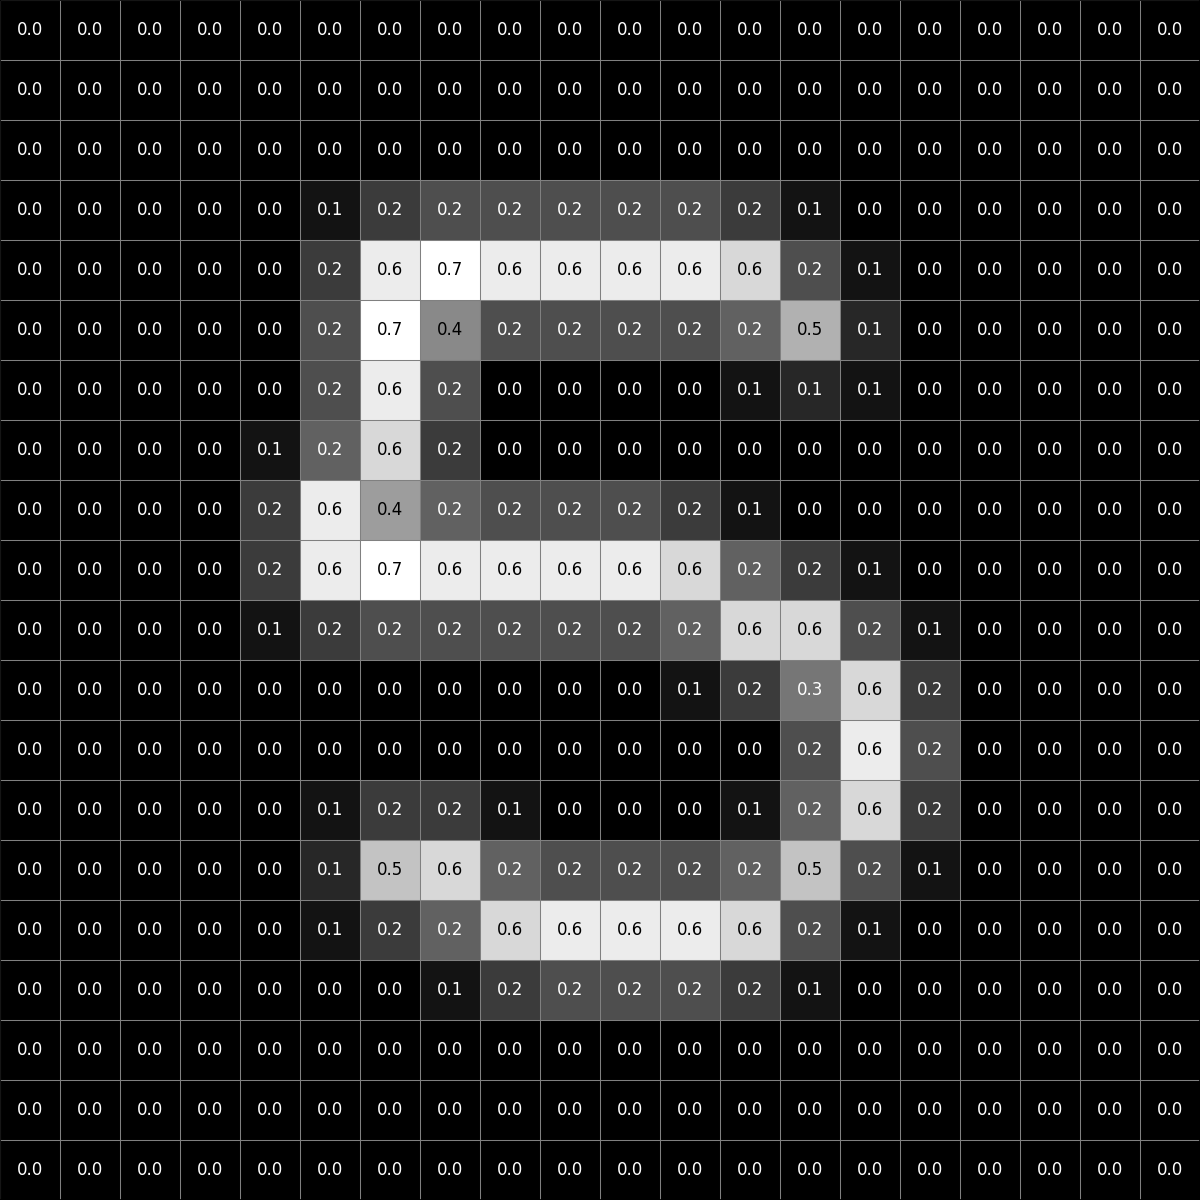
\includegraphics[width=6.2cm]{images/01_Input_Image/01_input_values.png}};
      \node[font=\fontsize{7}{8}\selectfont,text=PF,below=0.2cm of img2]
        {$20\!\times\!20$ grayscale --- with normalized values};

      % Text panel
      \fill[PA,rounded corners=4pt] (3.8,-1.8) rectangle (8.0,2.2);
      \fill[PB,rounded corners=3pt] (3.8,1.6) rectangle (8.0,2.2);
      \node[text=PH,font=\small\bfseries] at (5.9,1.9) {Numerical View};
      \node[text=PH,font=\fontsize{7}{8}\selectfont,text width=3.8cm,align=left]
        at (5.9,-0.1)
        {Each pixel is rescaled to\\the range \textbf{[0.0, 1.0]}.\\[5pt]
         \textbf{0.0} $\rightarrow$ pure black\\
         \textbf{1.0} $\rightarrow$ pure white\\[5pt]
         $20\!\times\!20 = 400$ floats form\\the network's \textbf{input}.\\[5pt]
         Normalization ensures\\stable gradients and\\\textbf{faster convergence}.};
    }

  \end{tikzpicture}
\end{frame}

% ================================================================
%  DEMO SLIDE 2 — CONVOLUTION: HORIZONTAL EDGE FILTER
% ================================================================
\begin{frame}{Convolution --- Horizontal Edge Detection}
  \begin{tikzpicture}

    % --- Info Block ---
    \node[fill=PA, text=PH, font=\bfseries\scriptsize, anchor=south west, text width=12.2cm, inner xsep=6pt, inner ysep=1.5pt] (boxhead) at (-5.8, 3.3) {{Key Insight}};
    \node[fill=PB!10, text=black, font=\scriptsize, anchor=north west, text width=12.2cm, inner xsep=6pt, inner ysep=1.5pt] (boxbody) at (boxhead.south west) {Extracts horizontal edges to identify features like the top bar of a 5.};
    % Input image (always visible, fixed position)
    \node[inner sep=0pt] (input) at (-4.2,0)
      {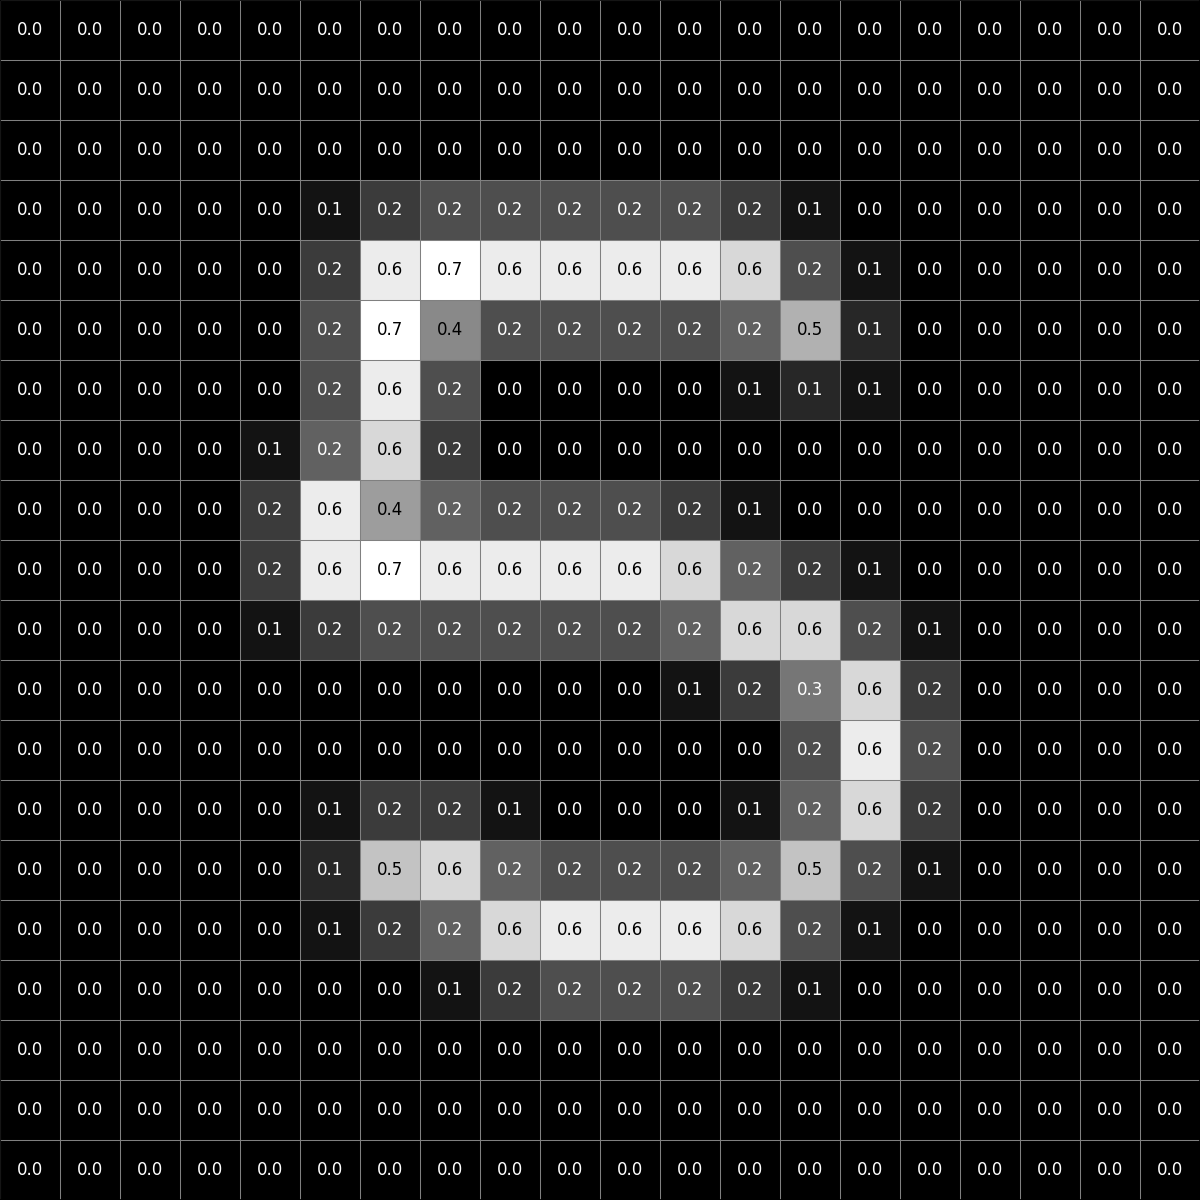
\includegraphics[width=4.5cm]{images/01_Input_Image/01_input_values.png}};
    \node[font=\fontsize{6}{7}\selectfont,text=PF,below=0.15cm of input]
      {Input $20\!\times\!20$};

    % Arrow + filter (overlay 2+)
    \only<2->{
      \draw[-{Stealth},line width=1.2pt,PB] (-1.6,0) -- (-0.6,0);
      \node[inner sep=0pt] (kernel) at (0.55,0)
        {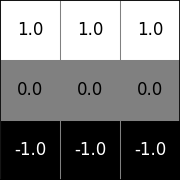
\includegraphics[width=1.8cm]{images/02_Conv1_Filters_and_Outputs/00_filter_horizontal_values.png}};
      \node[font=\fontsize{6}{7}\selectfont,text=PF,below=0.15cm of kernel]
        {Filter $3\!\times\!3$};
    }

    % Arrow + output (overlay 3)
    \only<3>{
      \draw[-{Stealth},line width=1.2pt,PB] (1.7,0) -- (2.7,0);
      \node[font=\fontsize{6}{7}\selectfont,text=PF] at (2.2,0.3) {$\ast$};
      \node[inner sep=0pt] (output) at (5.25,0)
        {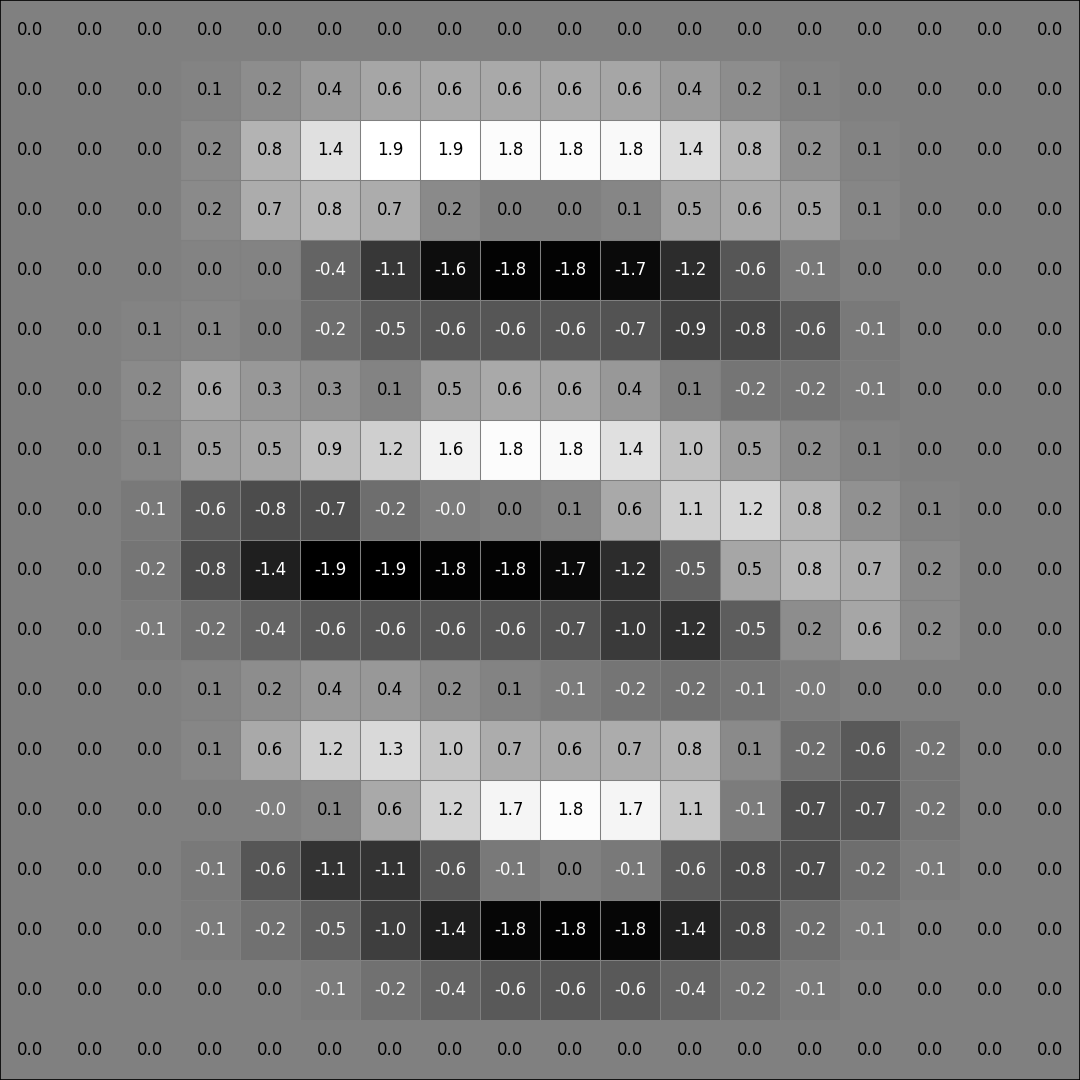
\includegraphics[width=4.5cm]{images/02_Conv1_Filters_and_Outputs/02_conv_horizontal_out_values.png}};
      \node[font=\fontsize{6}{7}\selectfont,text=PF,below=0.15cm of output]
        {Feature Map $18\!\times\!18$};
    }

  \end{tikzpicture}
\end{frame}

% ================================================================
%  DEMO SLIDE 3 — CONVOLUTION: VERTICAL EDGE FILTER
% ================================================================
\begin{frame}{Convolution --- Vertical Edge Detection}
  \begin{tikzpicture}

    % --- Info Block ---
    \node[fill=PA, text=PH, font=\bfseries\scriptsize, anchor=south west, text width=12.2cm, inner xsep=6pt, inner ysep=1.5pt] (boxhead) at (-5.8, 3.3) {{Key Insight}};
    \node[fill=PB!10, text=black, font=\scriptsize, anchor=north west, text width=12.2cm, inner xsep=6pt, inner ysep=1.5pt] (boxbody) at (boxhead.south west) {Highlights vertical structures to identify features like the straight back of a 1 or stem of a 5.};

    % Input image (always visible, fixed position)
    \node[inner sep=0pt] (input) at (-4.2,0)
      {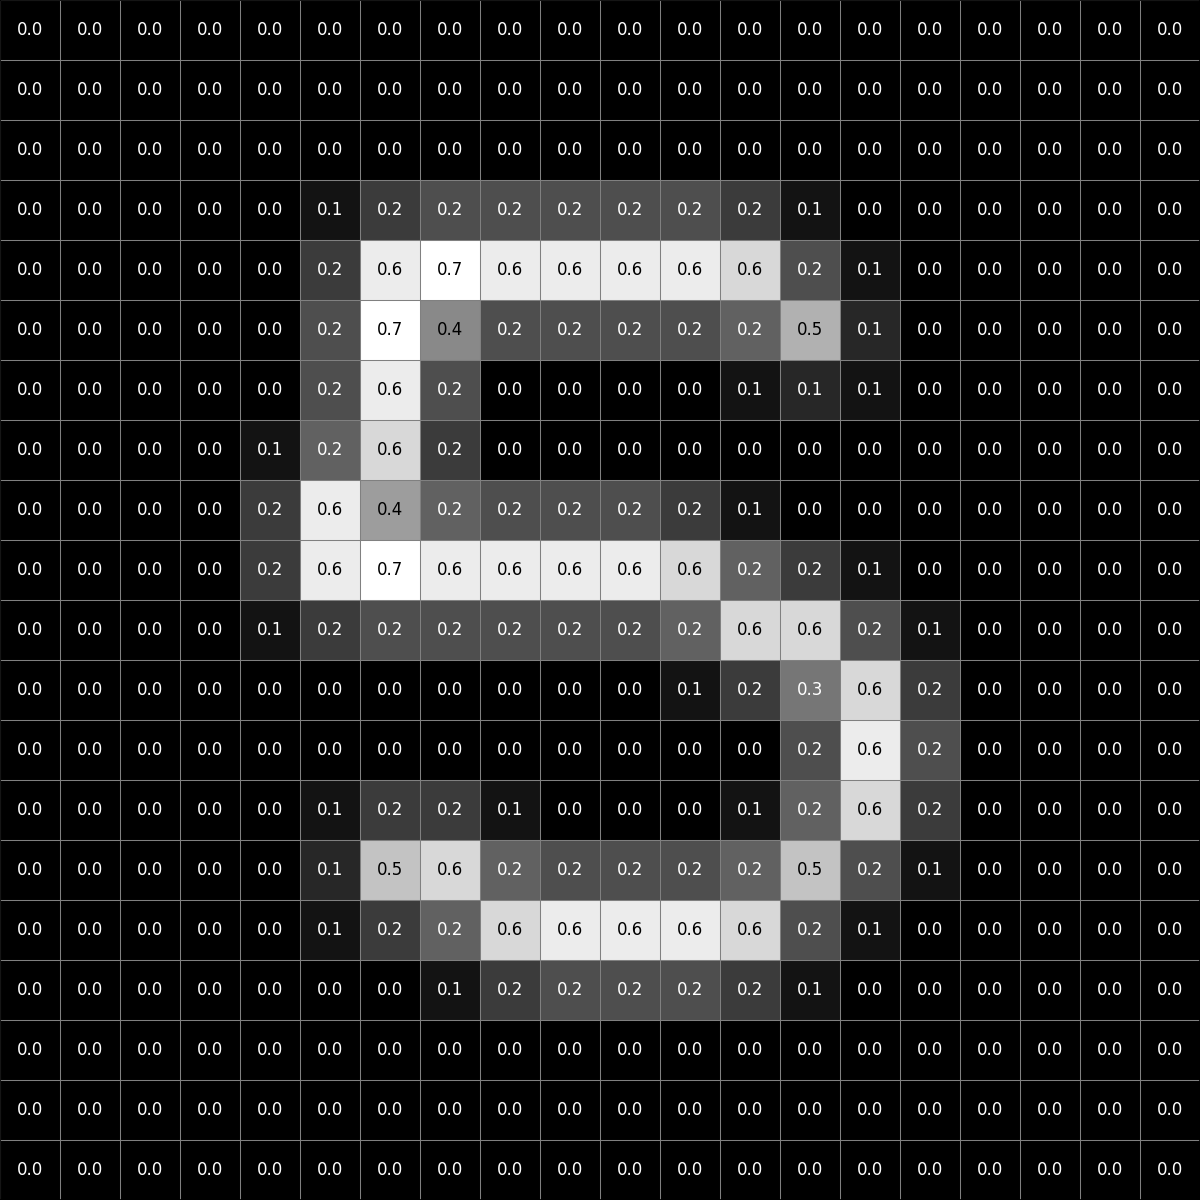
\includegraphics[width=4.5cm]{images/01_Input_Image/01_input_values.png}};
    \node[font=\fontsize{6}{7}\selectfont,text=PF,below=0.15cm of input]
      {Input $20\!\times\!20$};

    % Arrow + filter (overlay 2+)
    \only<2->{
      \draw[-{Stealth},line width=1.2pt,PB] (-1.6,0) -- (-0.6,0);
      \node[inner sep=0pt] (kernel) at (0.55,0)
        {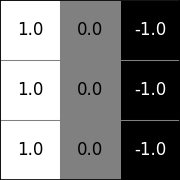
\includegraphics[width=1.8cm]{images/02_Conv1_Filters_and_Outputs/00_filter_vertical_values.png}};
      \node[font=\fontsize{6}{7}\selectfont,text=PF,below=0.15cm of kernel]
        {Filter $3\!\times\!3$};
    }

    % Arrow + output (overlay 3)
    \only<3>{
      \draw[-{Stealth},line width=1.2pt,PB] (1.7,0) -- (2.7,0);
      \node[font=\fontsize{6}{7}\selectfont,text=PF] at (2.2,0.3) {$\ast$};
      \node[inner sep=0pt] (output) at (5.25,0)
        {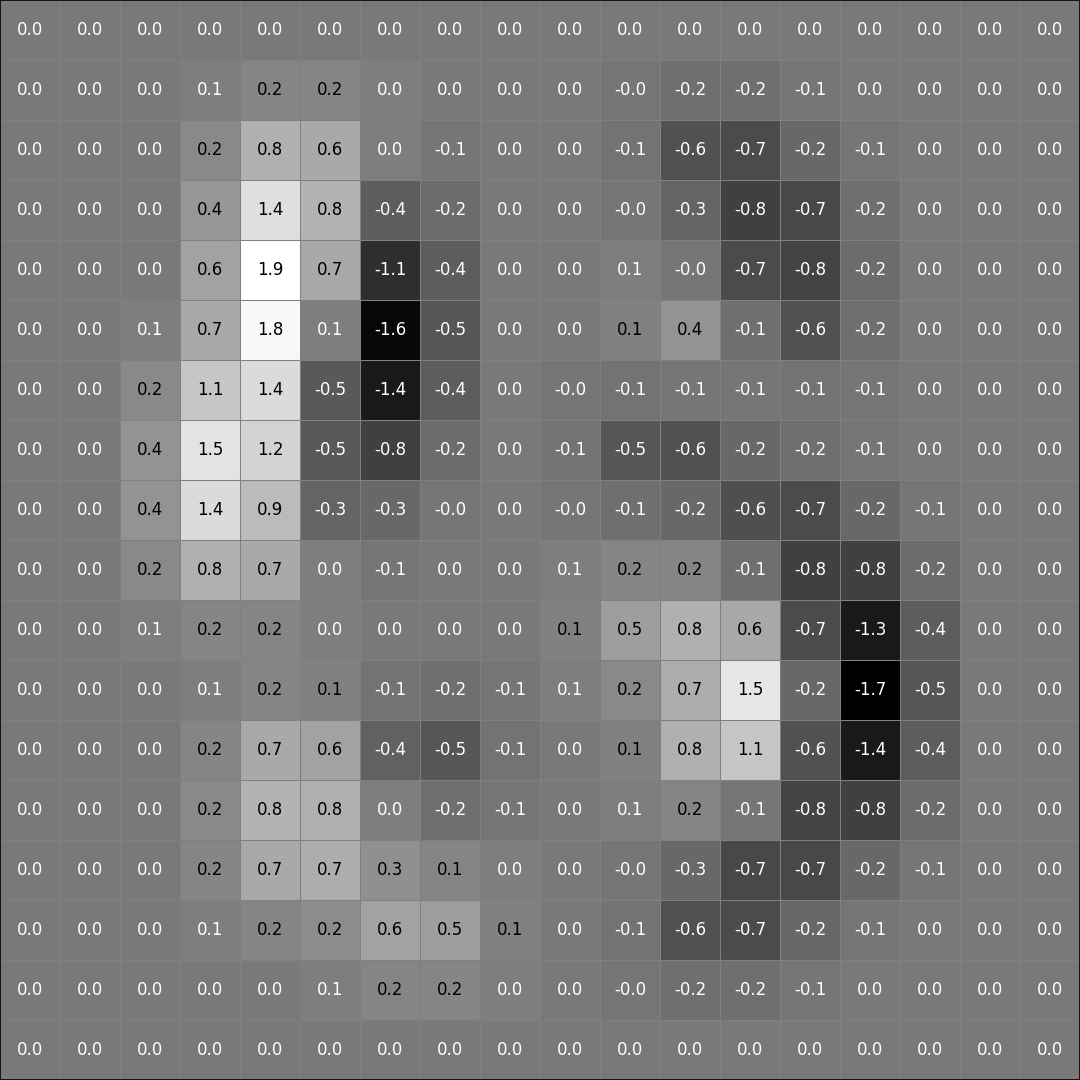
\includegraphics[width=4.5cm]{images/02_Conv1_Filters_and_Outputs/02_conv_vertical_out_values.png}};
      \node[font=\fontsize{6}{7}\selectfont,text=PF,below=0.15cm of output]
        {Feature Map $18\!\times\!18$};
    }

  \end{tikzpicture}
\end{frame}

% ================================================================
%  DEMO SLIDE 4 — CONVOLUTION: CORNER FILTER
% ================================================================
\begin{frame}{Convolution --- Corner Detection}
  \begin{tikzpicture}

    % --- Info Block ---
    \node[fill=PA, text=PH, font=\bfseries\scriptsize, anchor=south west, text width=12.2cm, inner xsep=6pt, inner ysep=1.5pt] (boxhead) at (-5.8, 3.3) {{Key Insight}};
    \node[fill=PB!10, text=black, font=\scriptsize, anchor=north west, text width=12.2cm, inner xsep=6pt, inner ysep=1.5pt] (boxbody) at (boxhead.south west) {Detects intersecting lines and sharp bends, crucial for recognizing loops in digits like 8 or 6.};

    % Input image (always visible, fixed position)
    \node[inner sep=0pt] (input) at (-4.2,0)
      {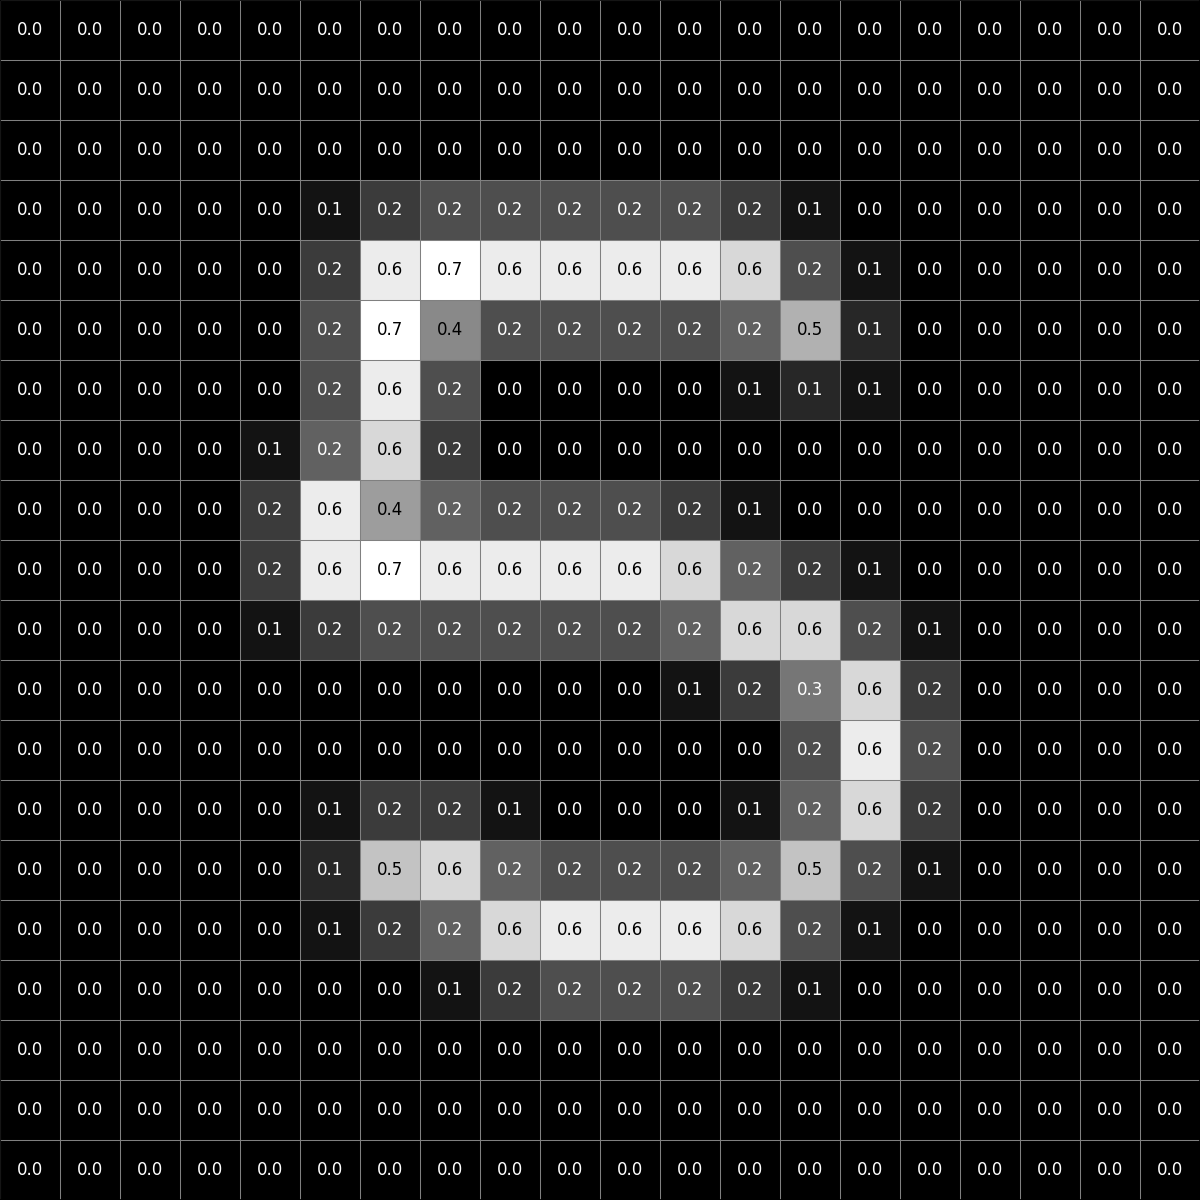
\includegraphics[width=4.5cm]{images/01_Input_Image/01_input_values.png}};
    \node[font=\fontsize{6}{7}\selectfont,text=PF,below=0.15cm of input]
      {Input $20\!\times\!20$};

    % Arrow + filter (overlay 2+)
    \only<2->{
      \draw[-{Stealth},line width=1.2pt,PB] (-1.6,0) -- (-0.6,0);
      \node[inner sep=0pt] (kernel) at (0.55,0)
        {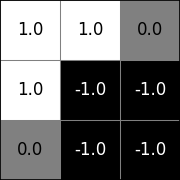
\includegraphics[width=1.8cm]{images/02_Conv1_Filters_and_Outputs/00_filter_corner_values.png}};
      \node[font=\fontsize{6}{7}\selectfont,text=PF,below=0.15cm of kernel]
        {Filter $3\!\times\!3$};
    }

    % Arrow + output (overlay 3)
    \only<3>{
      \draw[-{Stealth},line width=1.2pt,PB] (1.7,0) -- (2.7,0);
      \node[font=\fontsize{6}{7}\selectfont,text=PF] at (2.2,0.3) {$\ast$};
      \node[inner sep=0pt] (output) at (5.25,0)
        {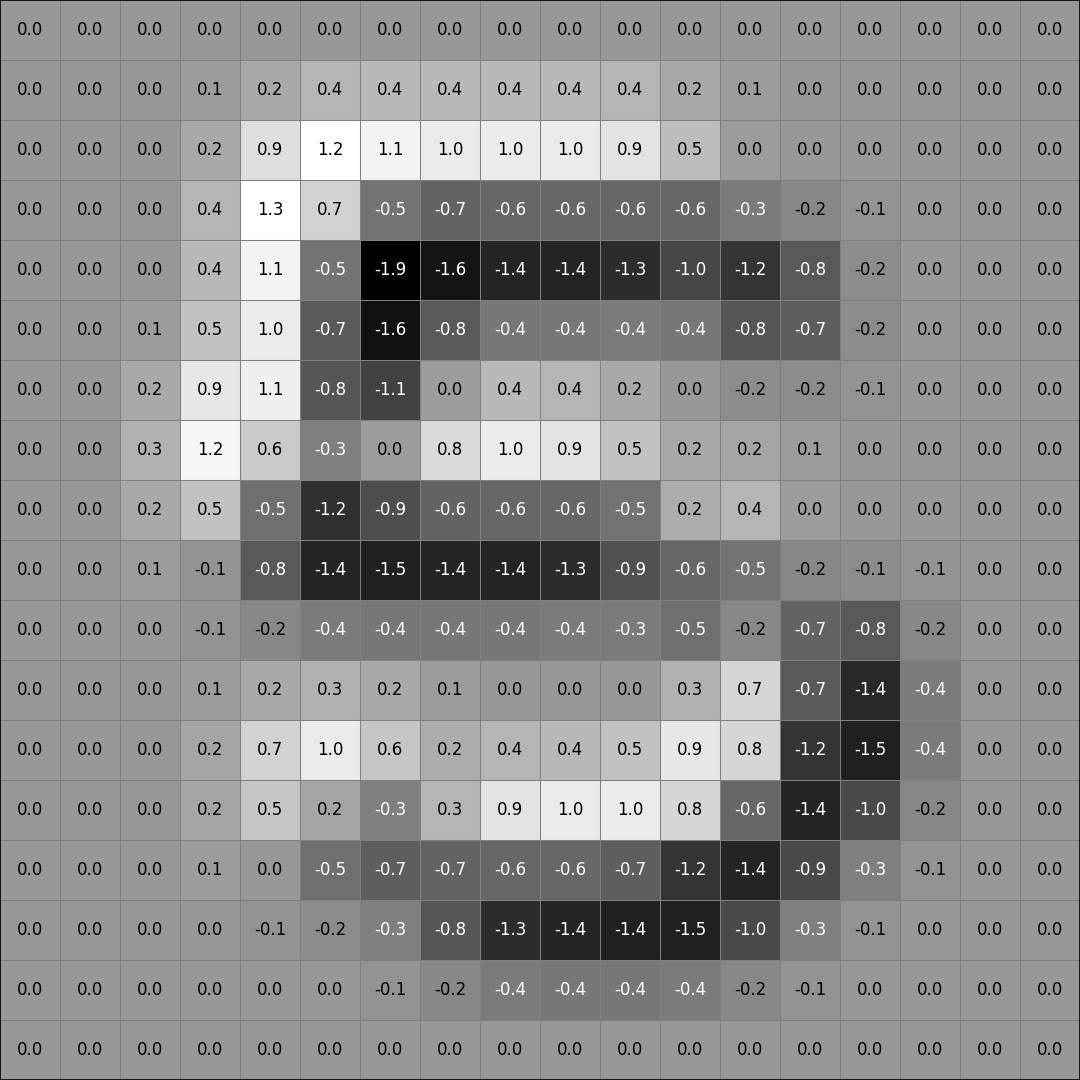
\includegraphics[width=4.5cm]{images/02_Conv1_Filters_and_Outputs/02_conv_corner_out_values.png}};
      \node[font=\fontsize{6}{7}\selectfont,text=PF,below=0.15cm of output]
        {Feature Map $18\!\times\!18$};
    }

  \end{tikzpicture}
\end{frame}


% ================================================================
%  DEMO SLIDE 5 — ReLU: HORIZONTAL FEATURE MAP
% ================================================================
\begin{frame}{ReLU --- Horizontal Feature Map}
  \begin{tikzpicture}

    % --- Info Block ---
    \node[fill=PA, text=PH, font=\bfseries\scriptsize, anchor=south west, text width=12.2cm, inner xsep=6pt, inner ysep=1.5pt] (boxhead) at (-5.8, 3.3) {{Key Insight}};
    \node[fill=PB!10, text=black, font=\scriptsize, anchor=north west, text width=12.2cm, inner xsep=6pt, inner ysep=1.5pt] (boxbody) at (boxhead.south west) {Removes negative values (noise) to keep only the most strongly detected horizontal features.};

    % Input (always visible)
    \node[inner sep=0pt] (input) at (-4.2,0)
      {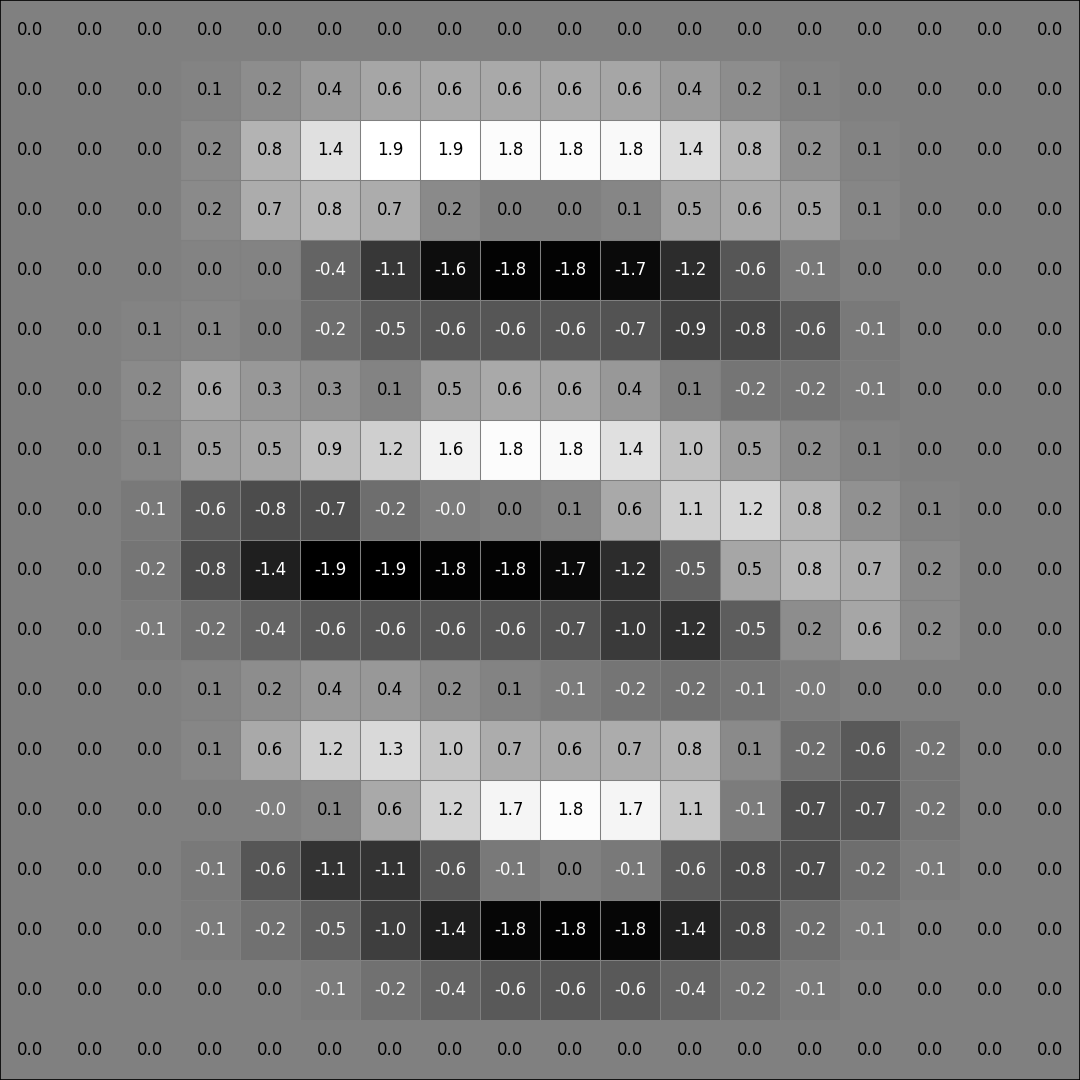
\includegraphics[width=4.5cm]{images/02_Conv1_Filters_and_Outputs/02_conv_horizontal_out_values.png}};
    \node[font=\fontsize{6}{7}\selectfont,text=PF,below=0.15cm of input]
      {Before ReLU};

    % Arrow (overlay 2+)
    \only<2->{
      \draw[-{Stealth},line width=1.2pt,PB] (-1.6,0) -- (0.4,0);
      \node[font=\fontsize{6}{7}\selectfont,text=PF] at (-0.6,0.35) {max(0,x)};
    }

    % Output (overlay 3)
    \only<3>{
      \node[inner sep=0pt] (output) at (3.0,0)
        {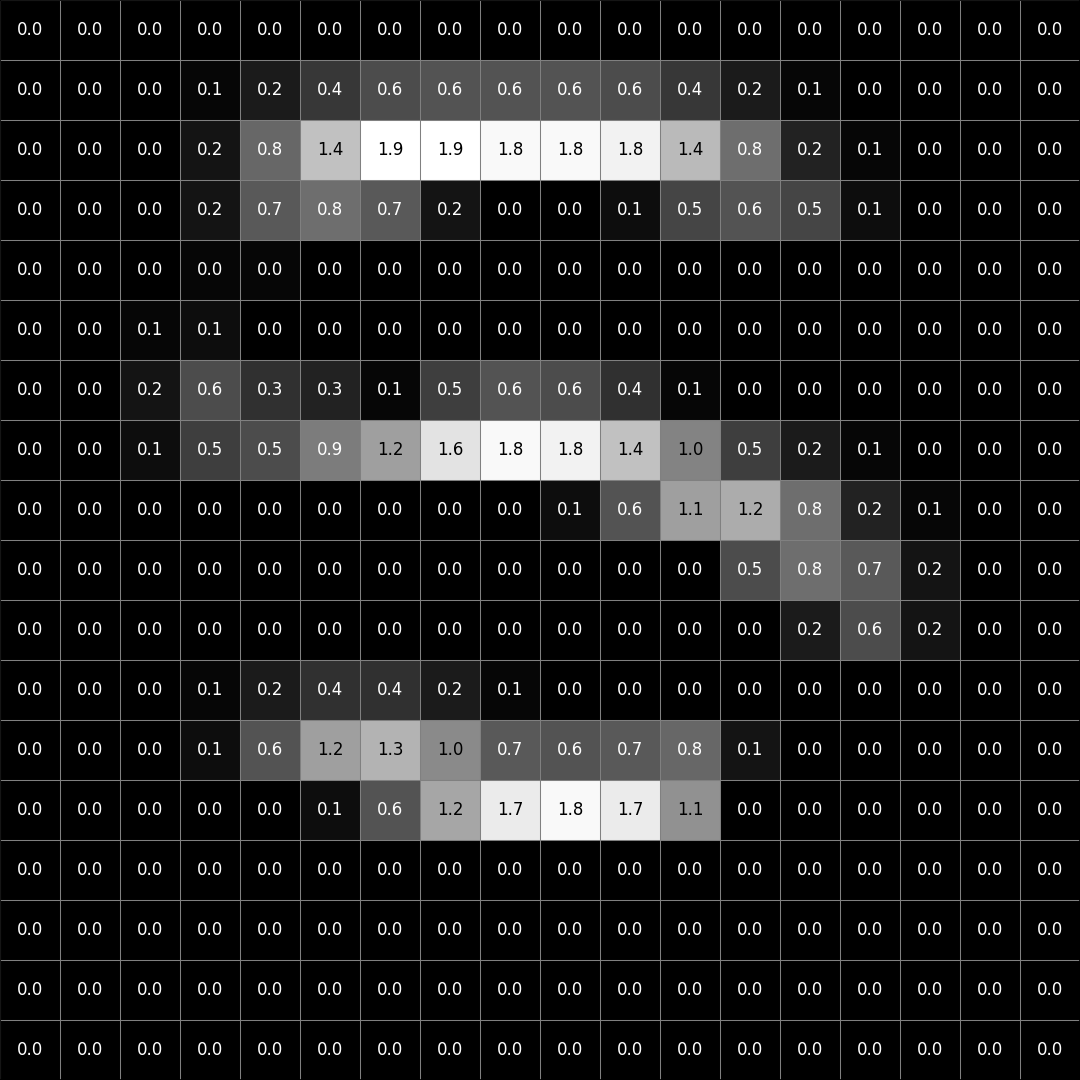
\includegraphics[width=4.5cm]{images/03_ReLU1/03_relu_horizontal_values.png}};
      \node[font=\fontsize{6}{7}\selectfont,text=PF,below=0.15cm of output]
        {After ReLU};
    }

  \end{tikzpicture}
\end{frame}

% ================================================================
%  DEMO SLIDE 6 — ReLU: VERTICAL FEATURE MAP
% ================================================================
\begin{frame}{ReLU --- Vertical Feature Map}
  \begin{tikzpicture}

    % --- Info Block ---
    \node[fill=PA, text=PH, font=\bfseries\scriptsize, anchor=south west, text width=12.2cm, inner xsep=6pt, inner ysep=1.5pt] (boxhead) at (-5.8, 3.3) {{Key Insight}};
    \node[fill=PB!10, text=black, font=\scriptsize, anchor=north west, text width=12.2cm, inner xsep=6pt, inner ysep=1.5pt] (boxbody) at (boxhead.south west) {Removes negative values (noise) to keep only the most strongly detected vertical features.};

    % Input
    \node[inner sep=0pt] (input) at (-4.2,0)
      {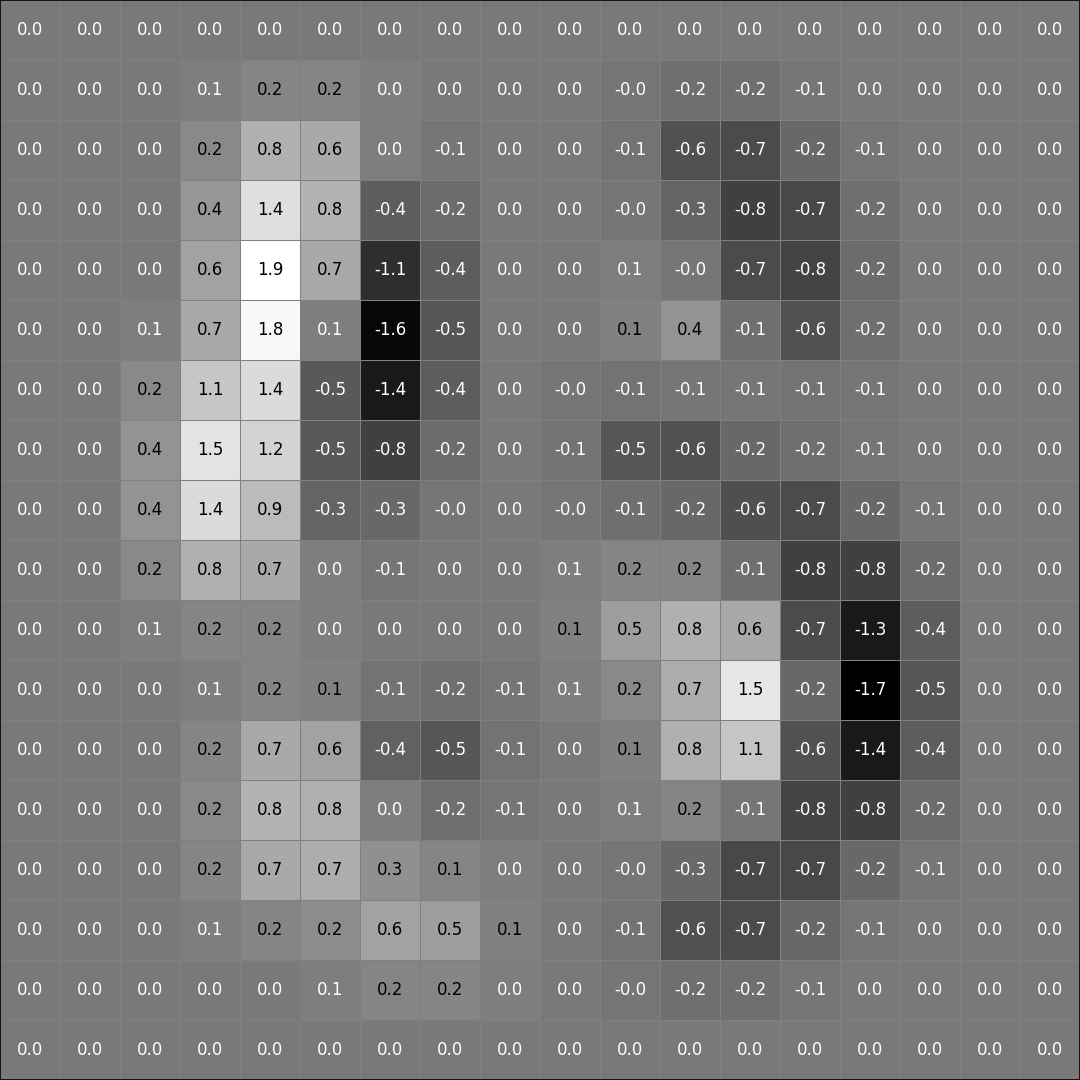
\includegraphics[width=4.5cm]{images/02_Conv1_Filters_and_Outputs/02_conv_vertical_out_values.png}};
    \node[font=\fontsize{6}{7}\selectfont,text=PF,below=0.15cm of input]
      {Before ReLU};

    % Arrow
    \only<2->{
      \draw[-{Stealth},line width=1.2pt,PB] (-1.6,0) -- (0.4,0);
      \node[font=\fontsize{6}{7}\selectfont,text=PF] at (-0.6,0.35) {max(0,x)};
    }
    
    % Output
    \only<3->{
      \node[inner sep=0pt] (output) at (3.0,0)
        {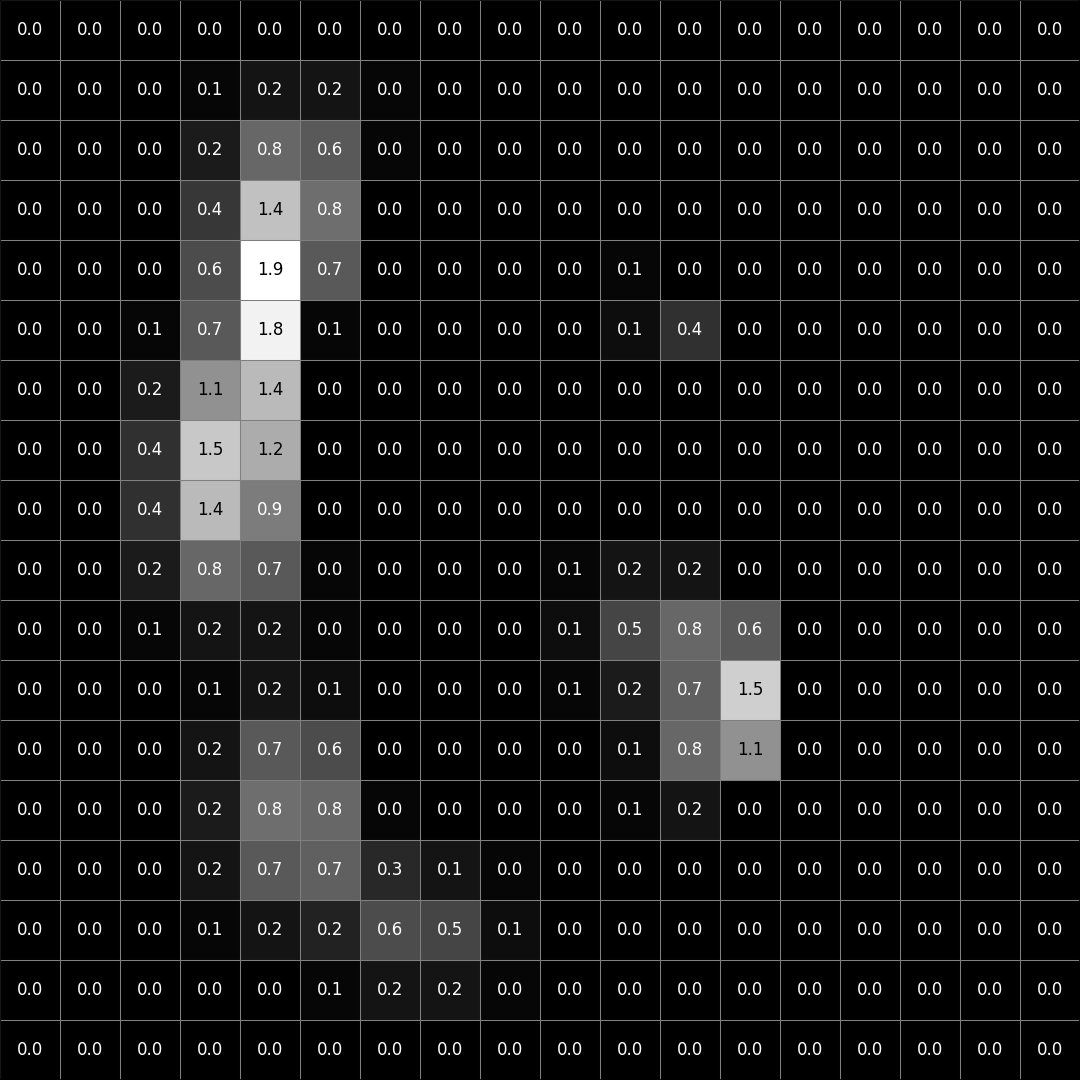
\includegraphics[width=4.5cm]{images/03_ReLU1/03_relu_vertical_values.png}};
      \node[font=\fontsize{6}{7}\selectfont,text=PF,below=0.15cm of output]
      {After ReLU};
    }

  \end{tikzpicture}
\end{frame}

% ================================================================
%  DEMO SLIDE 7 — ReLU: CORNER FEATURE MAP
% ================================================================
\begin{frame}{ReLU --- Corner Feature Map}
  \begin{tikzpicture}

    % --- Info Block ---
    \node[fill=PA, text=PH, font=\bfseries\scriptsize, anchor=south west, text width=12.2cm, inner xsep=6pt, inner ysep=1.5pt] (boxhead) at (-5.8, 3.3) {{Key Insight}};
    \node[fill=PB!10, text=black, font=\scriptsize, anchor=north west, text width=12.2cm, inner xsep=6pt, inner ysep=1.5pt] (boxbody) at (boxhead.south west) {Removes negative values (noise) to keep only the most strongly detected corner features.};

    % Input
    \node[inner sep=0pt] (input) at (-4.2,0)
      {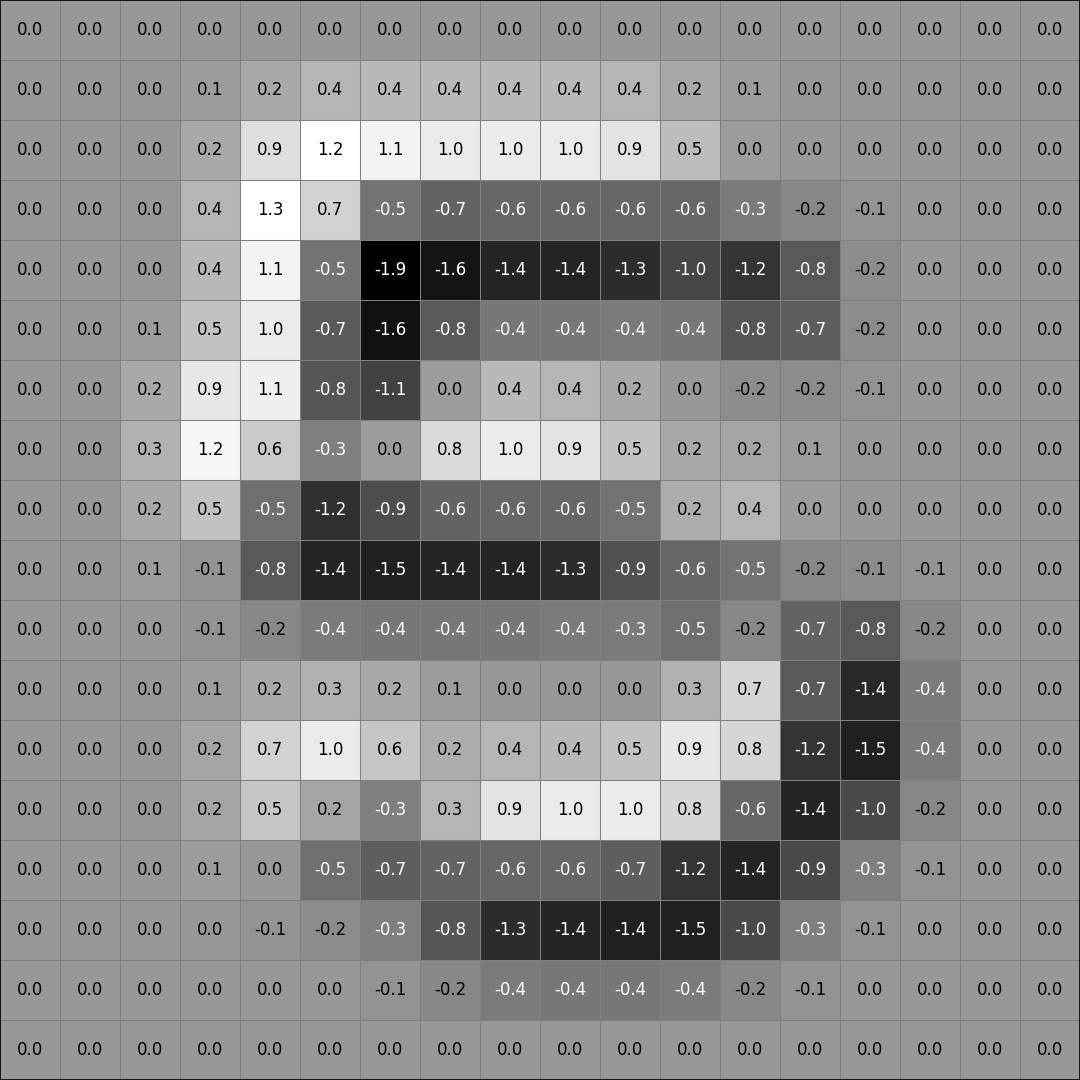
\includegraphics[width=4.5cm]{images/02_Conv1_Filters_and_Outputs/02_conv_corner_out_values.png}};
    \node[font=\fontsize{6}{7}\selectfont,text=PF,below=0.15cm of input]
      {Before ReLU};

    % Arrow
    \only<2->{
      \draw[-{Stealth},line width=1.2pt,PB] (-1.6,0) -- (0.4,0);
      \node[font=\fontsize{6}{7}\selectfont,text=PF] at (-0.6,0.35) {max(0,x)};
    }

    % Output
    \only<3->{
      \node[inner sep=0pt] (output) at (3.0,0)
        {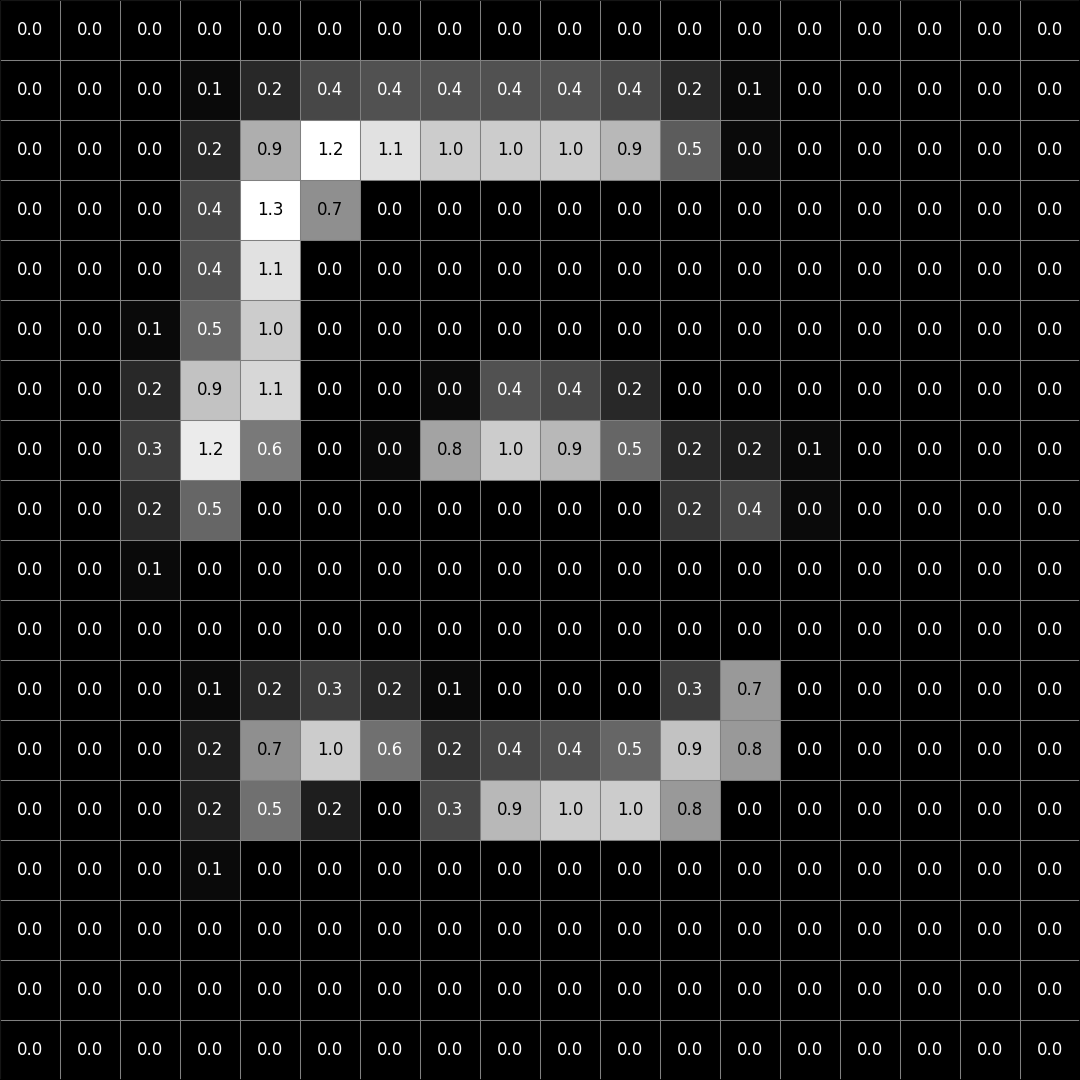
\includegraphics[width=4.5cm]{images/03_ReLU1/03_relu_corner_values.png}};
      \node[font=\fontsize{6}{7}\selectfont,text=PF,below=0.15cm of output]
        {After ReLU};
    }

  \end{tikzpicture}
\end{frame}

% ================================================================
%  DEMO SLIDE 8 — MERGE: SUM THREE ReLU FEATURE MAPS
% ================================================================
\begin{frame}{Merging Feature Maps}
  \begin{tikzpicture}

    % --- Info Block ---
    % \node[fill=PA, text=PH, font=\bfseries\scriptsize, anchor=south west, text width=12.2cm, inner xsep=6pt, inner ysep=1.5pt] (boxhead) at (-5.8, 3.3) {{Key Insight}};
    % \node[fill=PB!10, text=black, font=\scriptsize, anchor=north west, text width=12.2cm, inner xsep=6pt, inner ysep=1.5pt] (boxbody) at (boxhead.south west) {Removes negative values (noise) to keep only the most strongly detected corner features.};

    % ---- Three input images (smaller size, tighter spacing, labels shifted up) ----
    % Reduced width to 1.8cm and tightened y-coordinates to 2.0, 0, and -2.0
    \node[inner sep=0pt] (in1) at (-5.0, 2.0)
      {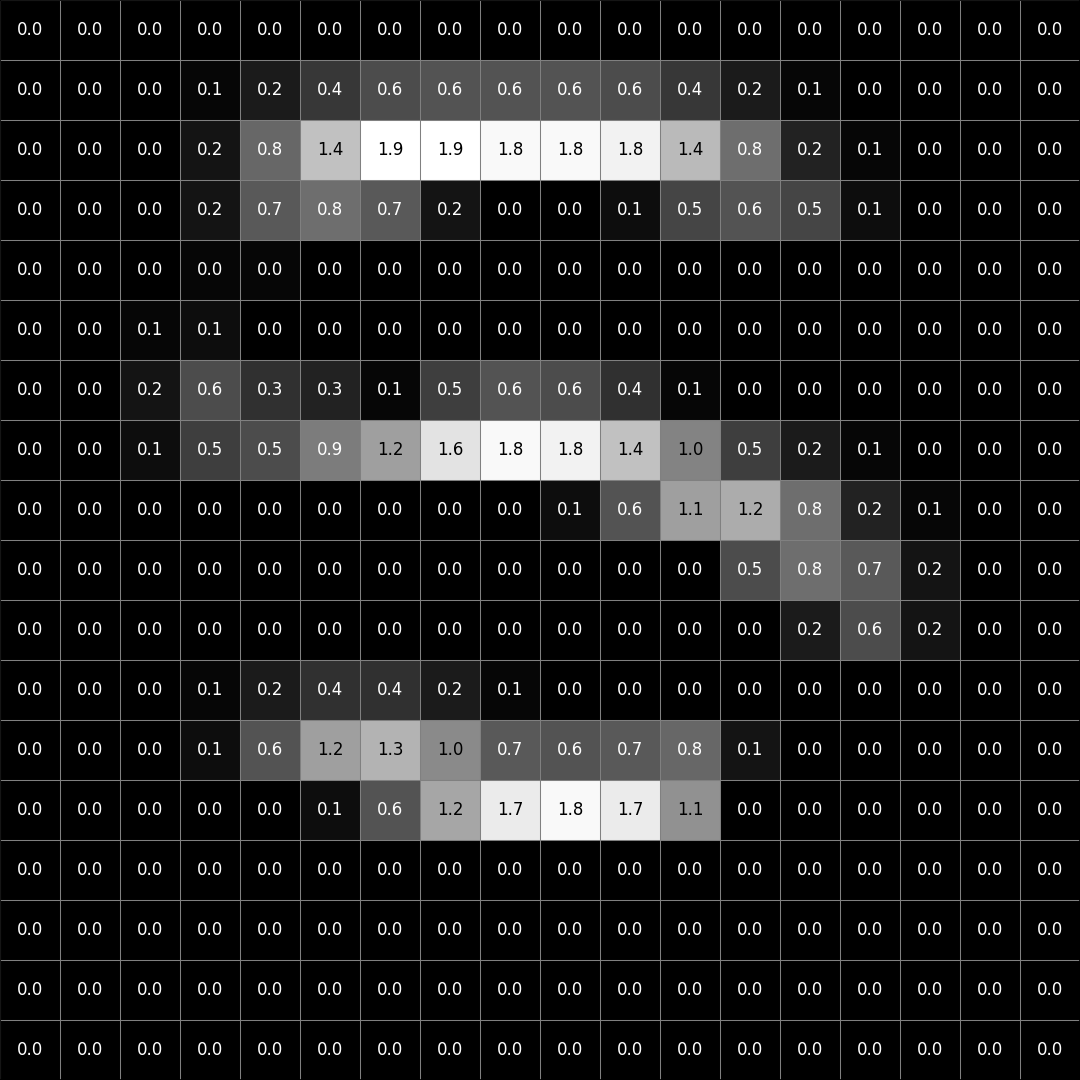
\includegraphics[width=1.8cm]{images/03_ReLU1/03_relu_horizontal_values.png}};
    \node[font=\fontsize{7}{8}\selectfont,text=PF,left=0.15cm of in1, yshift=0.5cm]
      {Horizontal};

    \node[inner sep=0pt] (in2) at (-5.0, 0)
      {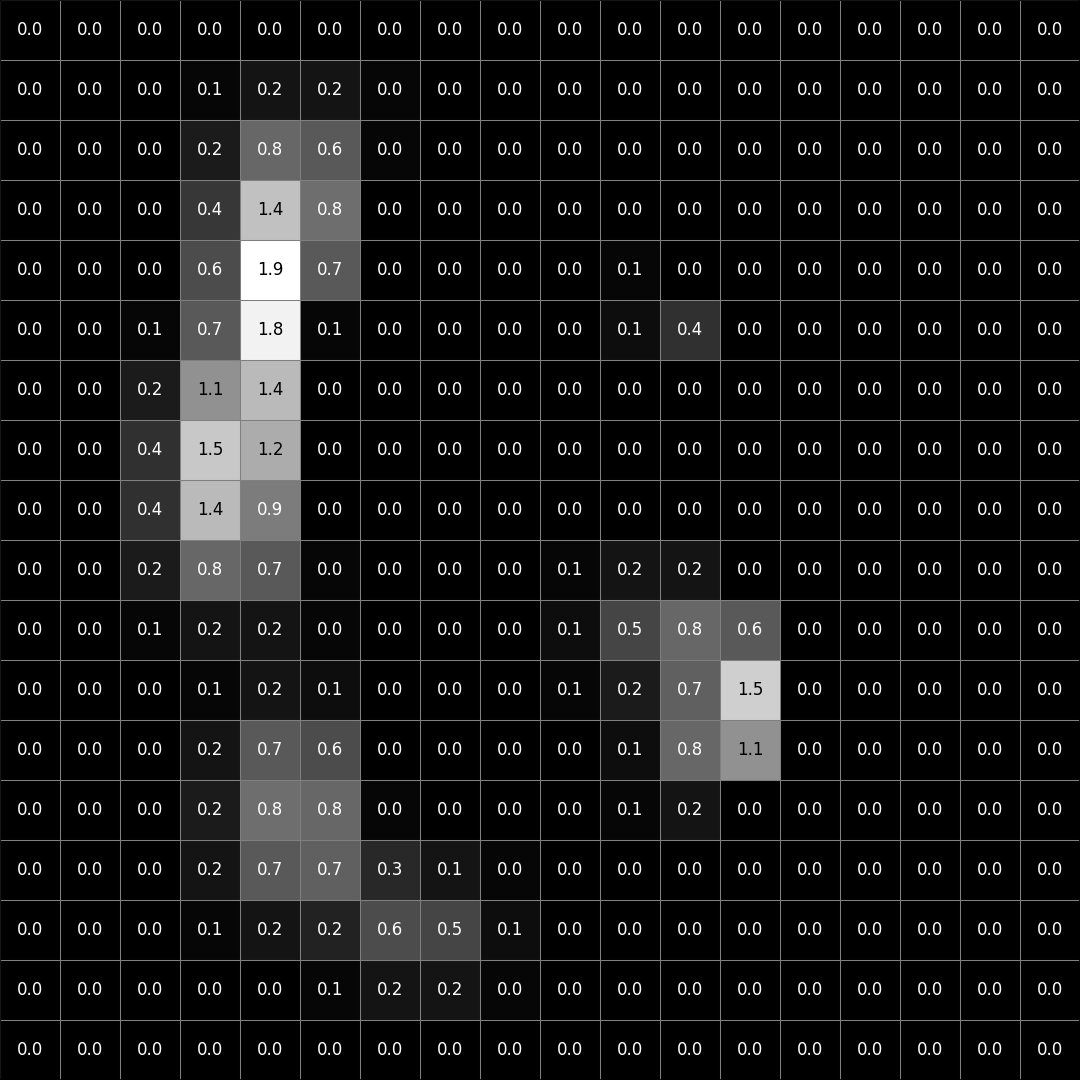
\includegraphics[width=1.8cm]{images/03_ReLU1/03_relu_vertical_values.png}};
    \node[font=\fontsize{7}{8}\selectfont,text=PF,left=0.15cm of in2, yshift=0.5cm]
      {Vertical};

    \node[inner sep=0pt] (in3) at (-5.0, -2.0)
      {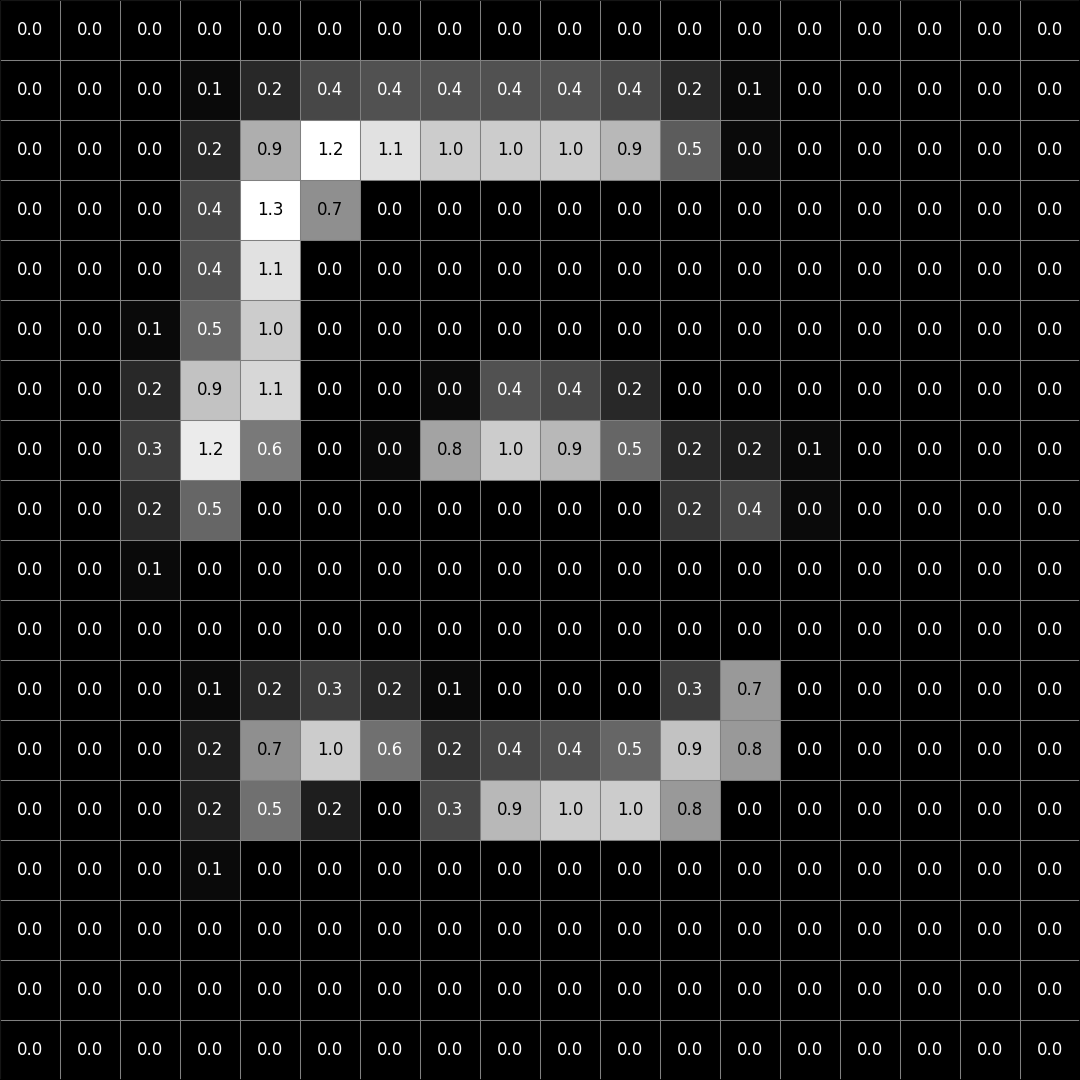
\includegraphics[width=1.8cm]{images/03_ReLU1/03_relu_corner_values.png}};
    \node[font=\fontsize{7}{8}\selectfont,text=PF,left=0.15cm of in3, yshift=0.5cm]
      {Corner};

    % ---- Arrows converging to summation (overlay 2+) ----
    \only<2->{
      % Start and end coordinates adjusted to match the tighter image spacing
      \draw[-{Stealth},line width=1.2pt,PB] (-3.9, 2.0)  -- (-2.6, 0.5);
      \draw[-{Stealth},line width=1.2pt,PB] (-3.9, 0)    -- (-2.6, 0);
      \draw[-{Stealth},line width=1.2pt,PB] (-3.9, -2.0) -- (-2.6, -0.5);

      % Summation symbol centered at y=0
      \node[fill=PD,text=PF,font=\Large\bfseries,
            rounded corners=4pt,inner sep=6pt] at (-2.0, 0) {$\Sigma$};
    }

    % ---- Arrow + output image (overlay 3) ----
    \only<3>{
      \draw[-{Stealth},line width=1.2pt,PB] (-1.4, 0) -- (-0.2, 0);

      % Reduced output width slightly to balance the smaller inputs
      \node[inner sep=0pt] (output) at (2.8, 0)
        {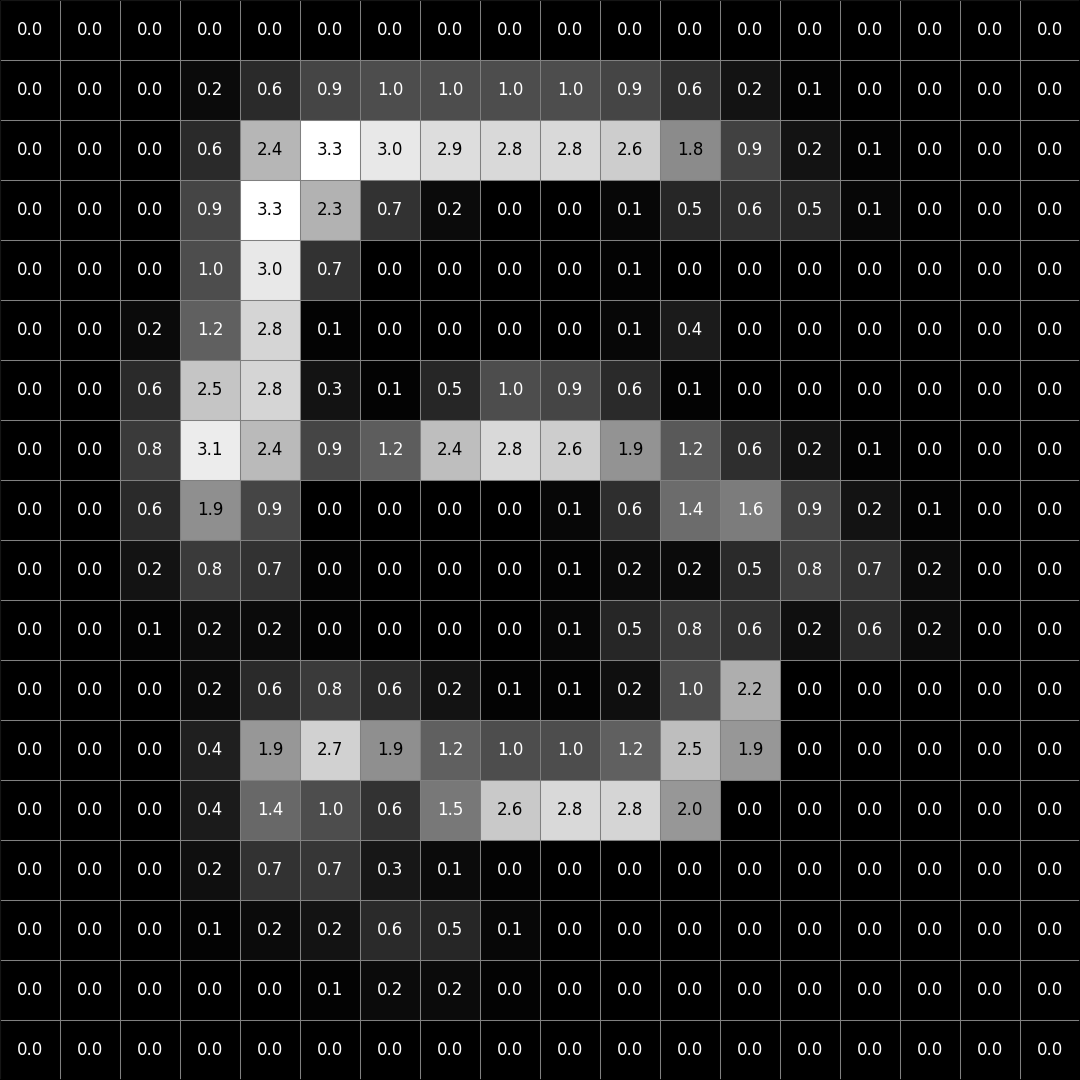
\includegraphics[width=5.0cm]{images/04_Merged_Features/04_merged_relu_features_values.png}};
      \node[font=\fontsize{6}{7}\selectfont,text=PF,below=0.15cm of output]
        {Merged Feature Map $18\!\times\!18$};
    }

  \end{tikzpicture}
\end{frame}

% ================================================================
%  DEMO SLIDE 11 — MAX POOLING + FLATTEN
% ================================================================
\begin{frame}{Max Pooling and Flattening}
  \begin{tikzpicture}

    % --- Info Block ---
    \node[fill=PA, text=PH, font=\bfseries\scriptsize, anchor=south west, text width=12.2cm, inner xsep=6pt, inner ysep=1.5pt] (boxhead) at (-5.8, 3.3) {{Key Insight}};
    \node[fill=PB!10, text=black, font=\scriptsize, anchor=north west, text width=12.2cm, inner xsep=6pt, inner ysep=1.5pt] (boxbody) at (boxhead.south west) {Downsamples to keep the most prominent features, then unrolls into a 1D list for the fully connected layer.};

    % Input (always visible)
    \node[inner sep=0pt] (input) at (-4.2,0)
      {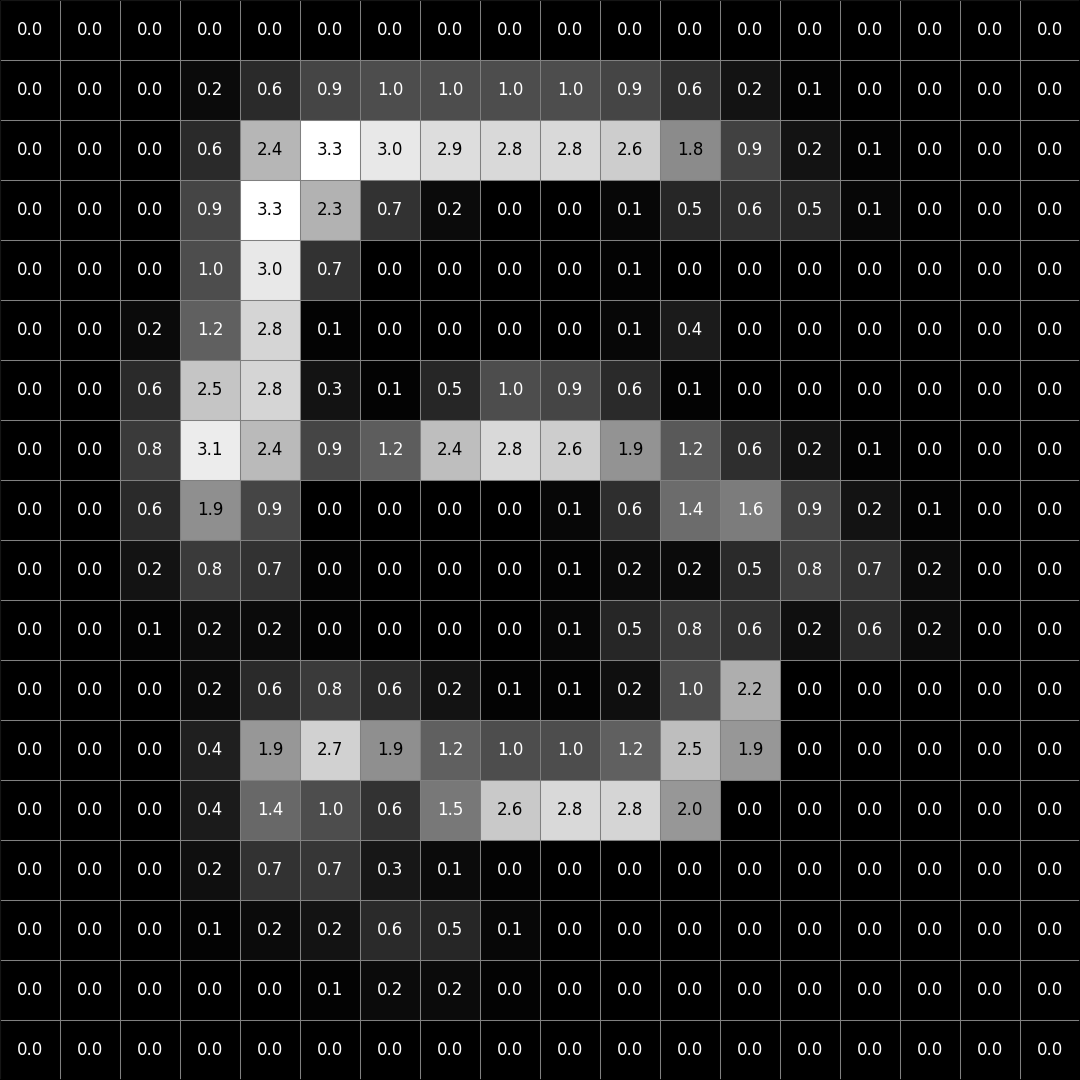
\includegraphics[width=4.5cm]{images/04_Merged_Features/04_merged_relu_features_values.png}};
    \node[font=\fontsize{6}{7}\selectfont,text=PF,below=0.15cm of input]
      {Before Pooling $18\!\times\!18$};

    % Arrow to pooled (overlay 2+)
    \only<2->{
      \draw[-{Stealth},line width=1.2pt,PB] (-1.6,0) -- (-0.1,0);
      \node[font=\fontsize{6}{7}\selectfont,text=PF] at (-0.9,0.37) {$2\!\times\!2$ max};
      \node[font=\fontsize{6}{7}\selectfont,text=PF] at (-0.9,0.17) {pooling};
    }

    % Pooled output (overlay 3+)
    \only<3->{
      \node[inner sep=0pt] (pooled) at (2.0,0)
        {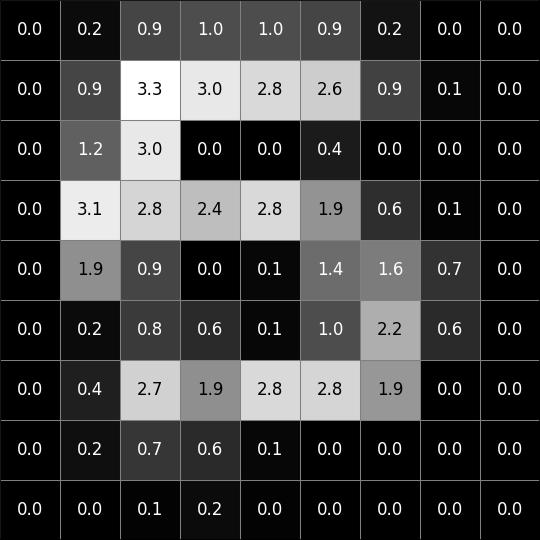
\includegraphics[width=3.5cm]{images/05_MaxPooling/05_maxpool_values.png}};
      \node[font=\fontsize{6}{7}\selectfont,text=PF,below=0.15cm of pooled]
        {After Pooling $9\!\times\!9$};
    }

    % Arrow to flattened (overlay 4+)
    \only<4->{
      \draw[-{Stealth},line width=1.2pt,PB] (4.1,0) -- (5.6,0);
      \node[font=\fontsize{5}{6}\selectfont,text=PF] at (4.8,0.3) {flatten};
    }

    % Flattened output (overlay 5)
    \only<5>{
      \node[inner sep=0pt] (flat) at (6.2,0)
        {
\includegraphics[height=5cm]{images/06_Flatten/06_flatten_values.png}};
      \node[font=\fontsize{5}{6}\selectfont,text=PF,below=0.01cm of flat]
        {$81\!\times\!1$};
    }

  \end{tikzpicture}
\end{frame}


% ================================================================
%  DEMO SLIDE 12 — FULLY CONNECTED LAYER + SOFTMAX OUTPUT
% ================================================================
\begin{frame}{Fully Connected Layer and Softmax}
  \begin{tikzpicture}

    % --- Info Block ---
    \node[fill=PA, text=PH, font=\bfseries\scriptsize, anchor=south west, text width=12.2cm, inner xsep=6pt, inner ysep=1.5pt] (boxhead) at (-5.8, 3.5) {{Key Insight}};
    \node[fill=PB!10, text=black, font=\scriptsize, anchor=north west, text width=12.2cm, inner xsep=6pt, inner ysep=1.5pt] (boxbody) at (boxhead.south west) {Weighs features to calculate raw scores (logits) for each digit, then converts them to probabilities.};

    % ---- Flattened input (always visible) ----
    \node[inner sep=0pt] (flat) at (-5.8,0)
      {
\includegraphics[height=5.0cm]{images/06_Flatten/06_flatten_values.png}};
    \node[font=\fontsize{4}{5}\selectfont,text=PF,below=0.01cm of flat]
      {Flatten $81\!\times\!1$};

    % ---- Arrow to FC (overlay 2+) ----
    \only<2->{
      \draw[-{Stealth},line width=1.2pt,PD] (-5.1,0) -- (-4.5,0);
    }

    % ---- Neural network diagram (overlay 3+) ----
    \only<2->{
    \begin{scope}[yshift=0.18cm]
      % --- Connections: Input -> Hidden ---
      \foreach \iy in {2.2,1.8,1.4,1.0,0.6,0.2,-0.2,-0.6,-1.0,-1.4,-1.8,-2.2,-2.6} {
        \foreach \hy in {1.6,1.0,0.4,-0.2,-0.8,-1.4,-2.0} {
          \draw[PB!70,line width=0.25pt] (-4.0,\iy) -- (-2.2,\hy);
        }
      }
      % --- Connections: Hidden -> Output ---
      \foreach \hy in {1.6,1.0,0.4,-0.2,-0.8,-1.4,-2.0} {
        \foreach \oy in {2.0,1.5,1.0,0.5,0.0,-0.5,-1.0,-1.5,-2.0,-2.5} {
          \draw[PE!70,line width=0.25pt] (-2.2,\hy) -- (-0.4,\oy);
        }
      }

      % --- Input layer nodes ---
      \foreach \y in {2.2,1.8,1.4,1.0,0.6,0.2,-0.2,-0.6,-1.0,-1.4,-1.8,-2.2,-2.6} {
        \fill[PB] (-4.0,\y) circle (0.1);
      }

      % --- Hidden layer nodes ---
      \foreach \y in {1.6,1.0,0.4,-0.2,-0.8,-1.4,-2.0} {
        \fill[PD] (-2.2,\y) circle (0.14);
      }

      % --- Output layer nodes ---
      \foreach \y in {2.0,1.5,1.0,0.5,0.0,-0.5,-1.0,-1.5,-2.0,-2.5} {
        \fill[PE] (-0.4,\y) circle (0.12);
      }
    \end{scope}
    }
    % ---- Arrow to raw values (overlay 4+) ----
    \only<3->{
      \draw[-{Stealth},line width=1.2pt,PD] (0.0,0) -- (0.7,0);
    }

% ---- Raw output values (overlay 5+) ----
    \only<3->{
      \fill[PA,rounded corners=3pt] (0.9,-2.6) rectangle (2.8,2.4);
      \fill[PB,rounded corners=2pt] (0.9,1.85) rectangle (2.8,2.4);
      \node[text=PH,font=\fontsize{5}{6}\selectfont\bfseries] at (1.85,2.12)
        {Raw Scores};

      \node[font=\fontsize{6}{7}\selectfont,text=PH,anchor=west] at (1.15,1.45)
        {\textbf{0:}};
      \node[font=\fontsize{6}{7}\selectfont,text=PH,anchor=east] at (2.55,1.45)
        {$-0.2$};

      \node[font=\fontsize{6}{7}\selectfont,text=PH,anchor=west] at (1.15,1.02)
        {\textbf{1:}};
      \node[font=\fontsize{6}{7}\selectfont,text=PH,anchor=east] at (2.55,1.02)
        {$\phantom{-}1.3$};

      \node[font=\fontsize{6}{7}\selectfont,text=PH,anchor=west] at (1.15,0.59)
        {\textbf{2:}};
      \node[font=\fontsize{6}{7}\selectfont,text=PH,anchor=east] at (2.55,0.59)
        {$\phantom{-}0.8$};

      \node[font=\fontsize{6}{7}\selectfont,text=PH,anchor=west] at (1.15,0.16)
        {\textbf{3:}};
      \node[font=\fontsize{6}{7}\selectfont,text=PH,anchor=east] at (2.55,0.16)
        {$\phantom{-}2.2$};

      \node[font=\fontsize{6}{7}\selectfont,text=PH,anchor=west] at (1.15,-0.27)
        {\textbf{4:}};
      \node[font=\fontsize{6}{7}\selectfont,text=PH,anchor=east] at (2.55,-0.27)
        {$\phantom{-}2.1$};

      % Highlight bar for digit 5
      \fill[PE!20,rounded corners=2pt] (1.0,-0.82) rectangle (2.7,-0.48);
      \node[font=\fontsize{6}{7}\selectfont,text=PE,anchor=west] at (1.15,-0.65)
        {\textbf{5:}};
      \node[font=\fontsize{6}{7}\selectfont,text=PE,anchor=east] at (2.55,-0.65)
        {$\mathbf{\phantom{-}8.5}$};

      \node[font=\fontsize{6}{7}\selectfont,text=PH,anchor=west] at (1.15,-1.08)
        {\textbf{6:}};
      \node[font=\fontsize{6}{7}\selectfont,text=PH,anchor=east] at (2.55,-1.08)
        {$-0.5$};

      \node[font=\fontsize{6}{7}\selectfont,text=PH,anchor=west] at (1.15,-1.51)
        {\textbf{7:}};
      \node[font=\fontsize{6}{7}\selectfont,text=PH,anchor=east] at (2.55,-1.51)
        {$-1.4$};

      \node[font=\fontsize{6}{7}\selectfont,text=PH,anchor=west] at (1.15,-1.94)
        {\textbf{8:}};
      \node[font=\fontsize{6}{7}\selectfont,text=PH,anchor=east] at (2.55,-1.94)
        {$\phantom{-}1.3$};

      \node[font=\fontsize{6}{7}\selectfont,text=PH,anchor=west] at (1.15,-2.37)
        {\textbf{9:}};
      \node[font=\fontsize{6}{7}\selectfont,text=PH,anchor=east] at (2.55,-2.37)
        {$\phantom{-}0.9$};
    }
    % ---- Arrow to softmax (overlay 6+) ----
    \only<4->{
      \draw[-{Stealth},line width=1.2pt,PD] (3.0,0) -- (3.7,0);
      \node[font=\fontsize{4}{5}\selectfont\bfseries,text=PD] at (3.35,0.3) {softmax};
    }

    % ---- Probability output (overlay 7) ----
\only<4->{
  \fill[PA,rounded corners=3pt] (3.9,-2.6) rectangle (6.6,2.4);
  \fill[PB,rounded corners=2pt] (3.9,1.85) rectangle (6.6,2.4);
  \node[text=PH,font=\fontsize{5}{6}\selectfont\bfseries] at (5.25,2.12)
    {Predictions};

  \node[font=\fontsize{6}{7}\selectfont,text=PH,anchor=west] at (4.5,1.45)
    {\textbf{0:}};
  \node[font=\fontsize{6}{7}\selectfont,text=PH,anchor=east] at (6,1.45)
    {0.0002};

  \node[font=\fontsize{6}{7}\selectfont,text=PH,anchor=west] at (4.5,1.02)
    {\textbf{1:}};
  \node[font=\fontsize{6}{7}\selectfont,text=PH,anchor=east] at (6,1.02)
    {0.0007};

  \node[font=\fontsize{6}{7}\selectfont,text=PH,anchor=west] at (4.5,0.59)
    {\textbf{2:}};
  \node[font=\fontsize{6}{7}\selectfont,text=PH,anchor=east] at (6,0.59)
    {0.0005};

  \node[font=\fontsize{6}{7}\selectfont,text=PH,anchor=west] at (4.5,0.16)
    {\textbf{3:}};
  \node[font=\fontsize{6}{7}\selectfont,text=PH,anchor=east] at (6,0.16)
    {0.0018};

  \node[font=\fontsize{6}{7}\selectfont,text=PH,anchor=west] at (4.5,-0.27)
    {\textbf{4:}};
  \node[font=\fontsize{6}{7}\selectfont,text=PH,anchor=east] at (6,-0.27)
    {0.0017};

  % Highlight bar for digit 5
  \fill[PE!20,rounded corners=2pt] (4.0,-0.82) rectangle (6.5,-0.48);
  \node[font=\fontsize{6}{7}\selectfont,text=PE,anchor=west] at (4.5,-0.65)
    {\textbf{5:}};
  \node[font=\fontsize{6}{7}\selectfont,text=PE,anchor=east] at (6,-0.65)
    {\textbf{0.9938}};

  \node[font=\fontsize{6}{7}\selectfont,text=PH,anchor=west] at (4.5,-1.08)
    {\textbf{6:}};
  \node[font=\fontsize{6}{7}\selectfont,text=PH,anchor=east] at (6,-1.08)
    {0.0001};

  \node[font=\fontsize{6}{7}\selectfont,text=PH,anchor=west] at (4.5,-1.51)
    {\textbf{7:}};
  \node[font=\fontsize{6}{7}\selectfont,text=PH,anchor=east] at (6,-1.51)
    {0.0000};

  \node[font=\fontsize{6}{7}\selectfont,text=PH,anchor=west] at (4.5,-1.94)
    {\textbf{8:}};
  \node[font=\fontsize{6}{7}\selectfont,text=PH,anchor=east] at (6,-1.94)
    {0.0007};

  \node[font=\fontsize{6}{7}\selectfont,text=PH,anchor=west] at (4.5,-2.37)
    {\textbf{9:}};
  \node[font=\fontsize{6}{7}\selectfont,text=PH,anchor=east] at (6,-2.37)
    {0.0005};
}

  \end{tikzpicture}
\end{frame}

% ================================================================
%  SLIDE 7 — RESULTS & IMPACT
% ================================================================
\begin{frame}{Real-World Impact of CNNs}
  \begin{tikzpicture}

    % ---- Block 1: Healthcare (always visible) ----
    \fill[PA,rounded corners=5pt] (0,0) rectangle (4.3,4.4);
    \fill[PB,rounded corners=3pt] (0,3.8) rectangle (4.3,4.4);
    \node[text=PH,font=\fontsize{7}{8}\selectfont\bfseries] at (2.15,4.1)
      {HEALTHCARE};
    \node[text=PD,font=\fontsize{22}{24}\selectfont\bfseries] at (2.15,3.0)
      {94.5\%};
    \node[text=PC,font=\fontsize{7}{8}\selectfont,text width=3.8cm,align=center]
      at (2.15,2.1)
      {Accuracy in detecting\\diabetic retinopathy};
    \node[text=PH!60,font=\fontsize{6}{7}\selectfont,text width=3.8cm,align=center]
      at (2.15,1.2)
      {Google Health, 2016\\FDA-approved CNN systems\\now used in 40+ countries};
    % mini bar
    \fill[PH!20,rounded corners=1pt] (0.4,0.35) rectangle (3.9,0.6);
    \fill[PD,rounded corners=1pt]    (0.4,0.35) rectangle (3.55,0.6);
    % \node[text=PH,font=\fontsize{5}{6}\selectfont] at (2.15,0.47) {94.5 / 100};

    % ---- Block 2: Autonomous Vehicles ----
    \only<2->{
    \fill[PB,rounded corners=5pt] (4.6,0) rectangle (8.9,4.4);
    \fill[PD,rounded corners=3pt] (4.6,3.8) rectangle (8.9,4.4);
    \node[text=PF,font=\fontsize{7}{8}\selectfont\bfseries] at (6.75,4.1)
      {AUTONOMOUS VEHICLES};
    \node[text=PH,font=\fontsize{22}{24}\selectfont\bfseries] at (6.75,3.0)
      {40\%};
    \node[text=PH!80,font=\fontsize{7}{8}\selectfont,text width=3.8cm,align=center]
      at (6.75,2.1)
      {Reduction in accident rate\\with CNN-based perception};
    \node[text=PH!60,font=\fontsize{6}{7}\selectfont,text width=3.8cm,align=center]
      at (6.75,1.2)
      {Tesla, Waymo, Cruise\\Process 1TB+ sensor data/hr\\Real-time object detection};
    % progress bar
    \fill[PH!20,rounded corners=1pt] (4.9,0.35) rectangle (8.6,0.6);
    \fill[PD,rounded corners=1pt]    (4.9,0.35) rectangle (6.38,0.6);
    % \node[text=PH,font=\fontsize{5}{6}\selectfont] at (6.75,0.47)
      {40 / 100};
    }

    % ---- Block 3: Satellite & Agriculture ----
    \only<3->{
    \fill[PD!80,rounded corners=5pt] (9.2,0) rectangle (13.5,4.4);
    \fill[PA,rounded corners=3pt] (9.2,3.8) rectangle (13.5,4.4);
    \node[text=PH,font=\fontsize{7}{8}\selectfont\bfseries] at (11.35,4.1)
      {SATELLITE \& AGRICULTURE};
    \node[text=PF,font=\fontsize{22}{24}\selectfont\bfseries] at (11.35,3.0)
      {89\%};
    \node[text=PF,font=\fontsize{7}{8}\selectfont,text width=3.8cm,align=center]
      at (11.35,2.1)
      {Crop disease detection\\accuracy from aerial images};
    \node[text=PF,font=\fontsize{6}{7}\selectfont,text width=3.8cm,align=center]
      at (11.35,1.2)
      {PlantVillage dataset\\Deforestation monitoring\\Yield prediction $\pm$5\%};
    % progress bar
    \fill[PI,rounded corners=1pt]  (9.5,0.35) rectangle (13.2,0.6);
    \fill[PA,rounded corners=1pt]  (9.5,0.35) rectangle (12.8,0.6);
    % \node[text=PH,font=\fontsize{5}{6}\selectfont] at (11.35,0.47) {89 / 100};
    }

  \end{tikzpicture}
\end{frame}


% ================================================================
%  SLIDE 9 — CNN GROWTH OVER TIME (line chart + donut)
% ================================================================
\begin{frame}{CNN Adoption: Growth Over Time}
  \begin{columns}[c]
    \begin{column}{0.58\textwidth}
      \begin{tikzpicture}
        \begin{axis}[
          width=8.5cm, height=6cm,
          xlabel={\small Year},
          ylabel={\small Count (thousands)},
          xlabel style={font=\fontsize{7}{8}\selectfont,color=PF},
          ylabel style={font=\fontsize{7}{8}\selectfont,color=PF},
          tick label style={font=\fontsize{6}{7}\selectfont,color=PF},
          axis line style={color=PI},
          grid=major, grid style={color=PI!80,dashed},
          ymin=0, ymax=35,
          xmin=2011, xmax=2025,
          xtick={2012,2014,2016,2018,2020,2022,2024},
          legend style={at={(0.02,0.98)},anchor=north west,
            font=\fontsize{6}{7}\selectfont,draw=none,fill=none,
            cells={anchor=west}},
        ]
          \addlegendimage{PB,mark=*,mark size=2pt,line width=1.5pt}
          \addlegendentry{CNN-related publications}
          \addlegendimage{PD,mark=*,mark size=2pt,line width=1.2pt}
          \addlegendentry{Industry deployments}

          \only<1->{\addplot[PB,mark=*,mark size=2pt,line width=1.5pt,forget plot]
            coordinates{(2012,1.2)};}
          \only<2->{\addplot[PB,mark=*,mark size=2pt,line width=1.5pt,forget plot]
            coordinates{(2012,1.2)(2014,3.8)};}
          \only<3->{\addplot[PB,mark=*,mark size=2pt,line width=1.5pt,forget plot]
            coordinates{(2012,1.2)(2014,3.8)(2016,8.5)};}
          \only<4->{\addplot[PB,mark=*,mark size=2pt,line width=1.5pt,forget plot]
            coordinates{(2012,1.2)(2014,3.8)(2016,8.5)(2018,15.2)};}
          \only<5->{\addplot[PB,mark=*,mark size=2pt,line width=1.5pt,forget plot]
            coordinates{(2012,1.2)(2014,3.8)(2016,8.5)(2018,15.2)(2020,22.1)};}
          \only<6->{\addplot[PB,mark=*,mark size=2pt,line width=1.5pt,forget plot]
            coordinates{(2012,1.2)(2014,3.8)(2016,8.5)(2018,15.2)(2020,22.1)(2022,28.4)};}
          \only<7->{\addplot[PB,mark=*,mark size=2pt,line width=1.5pt,forget plot]
            coordinates{(2012,1.2)(2014,3.8)(2016,8.5)(2018,15.2)(2020,22.1)(2022,28.4)(2024,32.0)};}

          \only<1->{\addplot[PD,mark=*,mark size=2pt,line width=1.2pt,forget plot]
            coordinates{(2012,0.3)};}
          \only<2->{\addplot[PD,mark=*,mark size=2pt,line width=1.2pt,forget plot]
            coordinates{(2012,0.3)(2014,1.1)};}
          \only<3->{\addplot[PD,mark=*,mark size=2pt,line width=1.2pt,forget plot]
            coordinates{(2012,0.3)(2014,1.1)(2016,3.2)};}
          \only<4->{\addplot[PD,mark=*,mark size=2pt,line width=1.2pt,forget plot]
            coordinates{(2012,0.3)(2014,1.1)(2016,3.2)(2018,7.8)};}
          \only<5->{\addplot[PD,mark=*,mark size=2pt,line width=1.2pt,forget plot]
            coordinates{(2012,0.3)(2014,1.1)(2016,3.2)(2018,7.8)(2020,14.5)};}
          \only<6->{\addplot[PD,mark=*,mark size=2pt,line width=1.2pt,forget plot]
            coordinates{(2012,0.3)(2014,1.1)(2016,3.2)(2018,7.8)(2020,14.5)(2022,20.1)};}
          \only<7->{\addplot[PD,mark=*,mark size=2pt,line width=1.2pt,forget plot]
            coordinates{(2012,0.3)(2014,1.1)(2016,3.2)(2018,7.8)(2020,14.5)(2022,20.1)(2024,25.3)};}
        \end{axis}
      \end{tikzpicture}
    \end{column}
    \begin{column}{0.39\textwidth}
      \only<8->{
      \centering
      \begin{tikzpicture}[yscale=0.95]
        % Title
        \node[font=\small\bfseries,text=PA] at (2.0,5.6) {Architecture Usage};

        % Donut chart
        \def\R{1.3}\def\r{0.7}
        % ResNet 35% -> 126 deg
        \fill[PA] (2.0,3.8)--++(90:\R) arc[start angle=90,end angle=-36,radius=\R]
          --++(-36:-\R+\r) arc[start angle=-36,end angle=90,radius=\r]--cycle;
        % EfficientNet 25% -> 90 deg
        \fill[PB] (2.0,3.8)--++(-36:\R) arc[start angle=-36,end angle=-126,radius=\R]
          --++(-126:-\R+\r) arc[start angle=-126,end angle=-36,radius=\r]--cycle;
        % YOLO 20% -> 72 deg
        \fill[PD] (2.0,3.8)--++(-126:\R) arc[start angle=-126,end angle=-198,radius=\R]
          --++(-198:-\R+\r) arc[start angle=-198,end angle=-126,radius=\r]--cycle;
        % VGG 12% -> 43.2 deg
        \fill[PG] (2.0,3.8)--++(-198:\R) arc[start angle=-198,end angle=-241.2,radius=\R]
          --++(-241.2:-\R+\r) arc[start angle=-241.2,end angle=-198,radius=\r]--cycle;
        % Other 8% -> 28.8 deg
        \fill[PC] (2.0,3.8)--++(-241.2:\R) arc[start angle=-241.2,end angle=-270,radius=\R]
          --++(-270:-\R+\r) arc[start angle=-270,end angle=-241.2,radius=\r]--cycle;

        \node[text=PF,font=\fontsize{7}{8}\selectfont\bfseries] at (2.0,3.95) {2024};
        \node[text=PF,font=\fontsize{6}{7}\selectfont] at (2.0,3.6) {Survey};

        % Always reserve space for legend — show or phantom
        \fill[PA,rounded corners=1pt,opacity=\ifnum\value{beamerpauses}>8 1\else 0\fi]
          (0.2,1.8) rectangle (0.55,2.05);

        % Invisible anchor node to always reserve full height
        \node[opacity=0] at (0.2,0.0) {\phantom{X}};
        \node[opacity=0] at (0.2,2.05) {\phantom{X}};

        % Legend — appears one step after donut
        \only<9->{
          \fill[PA,rounded corners=1pt] (0.2,1.8) rectangle (0.55,2.05);
          \node[text=PF,font=\fontsize{6}{7}\selectfont,anchor=west] at (0.65,1.92)
            {ResNet --- 35\%};
          \fill[PB,rounded corners=1pt] (0.2,1.35) rectangle (0.55,1.60);
          \node[text=PF,font=\fontsize{6}{7}\selectfont,anchor=west] at (0.65,1.47)
            {EfficientNet --- 25\%};
          \fill[PD,rounded corners=1pt] (0.2,0.90) rectangle (0.55,1.15);
          \node[text=PF,font=\fontsize{6}{7}\selectfont,anchor=west] at (0.65,1.02)
            {YOLO --- 20\%};
          \fill[PG,rounded corners=1pt] (0.2,0.45) rectangle (0.55,0.70);
          \node[text=PF,font=\fontsize{6}{7}\selectfont,anchor=west] at (0.65,0.57)
            {VGG --- 12\%};
          \fill[PC,rounded corners=1pt] (0.2,0.0) rectangle (0.55,0.25);
          \node[text=PF,font=\fontsize{6}{7}\selectfont,anchor=west] at (0.65,0.12)
            {Other --- 8\%};
        }
      \end{tikzpicture}
      }
    \end{column}
  \end{columns}
\end{frame}


% ================================================================
%  SLIDE 10 — LIMITATIONS (block by block with overlays)
% ================================================================
\begin{frame}{Limitations of CNNs}
  \begin{tikzpicture}

        % ---- Block 1: Computational Cost (always visible) ----
    \fill[PA,rounded corners=5pt] (0,0) rectangle (4.3,4.4);
    \fill[PB,rounded corners=3pt] (0,3.8) rectangle (4.3,4.4);
    \node[text=PH,font=\fontsize{7}{8}\selectfont\bfseries] at (2.15,4.1)
      {COMPUTATIONAL COST};
    \node[text=PD,font=\fontsize{20}{22}\selectfont\bfseries] at (2.15,3.1)
      {300W+};
    \node[text=PC,font=\fontsize{7}{8}\selectfont,text width=3.8cm,align=center]
      at (2.15,2.2)
      {GPU power consumption\\during training};
    \node[text=PH!60,font=\fontsize{6}{7}\selectfont,text width=3.8cm,align=center]
      at (2.15,1.0)
      {GPT-scale models: \$10M+\\training cost; ResNet-152:\\60M parameters; days on\\8$\times$A100 GPUs};

    % ---- Block 2: Data Hunger ----
    \only<2->{
    \fill[PB,rounded corners=5pt] (4.6,0) rectangle (8.9,4.4);
    \fill[PD,rounded corners=3pt] (4.6,3.8) rectangle (8.9,4.4);
    \node[text=PF,font=\fontsize{7}{8}\selectfont\bfseries] at (6.75,4.1)
      {DATA HUNGER};
    \node[text=PH,font=\fontsize{20}{22}\selectfont\bfseries] at (6.75,3.1)
      {1M+};
    \node[text=PH!80,font=\fontsize{7}{8}\selectfont,text width=3.8cm,align=center]
      at (6.75,2.2)
      {Labeled images needed\\for robust training};
    \node[text=PH!60,font=\fontsize{6}{7}\selectfont,text width=3.8cm,align=center]
      at (6.75,1.0)
      {ImageNet: 14M images\\Medical data: scarce \& expensive\\Labeling cost: \$0.05--\$6/image\\Bias amplification risk};
    }

    % ---- Block 3: Interpretability ----
    \only<3->{
    \fill[PD!80,rounded corners=5pt] (9.2,0) rectangle (13.5,4.4);
    \fill[PA,rounded corners=3pt] (9.2,3.8) rectangle (13.5,4.4);
    \node[text=PH,font=\fontsize{7}{8}\selectfont\bfseries] at (11.35,4.1)
      {BLACK BOX PROBLEM};
    \node[text=PF,font=\fontsize{20}{22}\selectfont\bfseries] at (11.35,3.1)
      {87\%};
    \node[text=PF,font=\fontsize{7}{8}\selectfont,text width=3.8cm,align=center]
      at (11.35,2.2)
      {Of practitioners report\\difficulty explaining CNN\\decisions to stakeholders};
    \node[text=PF,font=\fontsize{6}{7}\selectfont,text width=3.8cm,align=center]
      at (11.35,1.0)
      {EU AI Act: explainability\\required for high-risk systems\\Grad-CAM helps but\\insufficient for regulation};
    }

  \end{tikzpicture}
\end{frame}



% ================================================================
%  SLIDE 10 — THANK YOU
% ================================================================
{
\setbeamertemplate{footline}{}
\begin{frame}[plain]
  \begin{tikzpicture}[remember picture,overlay]
    % Background
    \fill[PA] (current page.south west) rectangle (current page.north east);
    % Top-left circle decoration
    \fill[PB,opacity=0.92]
      ([xshift=-1.5cm,yshift=-1.5cm] current page.north west) circle (4.2cm);
    \fill[PA]
      ([xshift=-1.5cm,yshift=-1.5cm] current page.north west) circle (2.4cm);
    % Bottom-right triangle decoration
    \fill[PD,opacity=0.88]
      ([xshift=16cm] current page.south west) --
      ([xshift=16cm,yshift=5cm] current page.south west) --
      ([xshift=11cm] current page.south west) -- cycle;
    \fill[PE,opacity=0.65]
      ([xshift=15.5cm] current page.south west)
      rectangle (current page.north east);
    % Mid parallelogram
    \fill[PC,opacity=0.12]
      ([xshift=4cm,yshift=1cm] current page.south west) --
      ([xshift=9cm,yshift=1cm] current page.south west) --
      ([xshift=7cm,yshift=7cm] current page.south west) --
      ([xshift=2cm,yshift=7cm] current page.south west) -- cycle;
    % Divider line
    % \draw[PD,line width=2pt]
    %   ([xshift=4.5cm,yshift=3.2cm] current page.south west) --
    %   ([xshift=14.8cm,yshift=3.2cm] current page.south west);
    % Thank You text
    \node[anchor=west,text=PH,font=\fontsize{36}{40}\selectfont\bfseries,
          text width=10cm]
      at ([xshift=4.5cm,yshift=4.7cm] current page.south west)
      {Thank You};
    % Roll numbers
    \node[anchor=west,text=PH,font=\large,
          text width=10cm]
      at ([xshift=4.5cm,yshift=3.5cm] current page.south west)
      { ID: 2205031,\quad2205046,\quad2205059};
    % Bottom color bar
    \fill[PA] (current page.south west)
      rectangle ([xshift=2.28cm,yshift=0.55cm] current page.south west);
    \fill[PB] ([xshift=2.30cm] current page.south west)
      rectangle ([xshift=4.58cm,yshift=0.55cm] current page.south west);
    \fill[PC] ([xshift=4.60cm] current page.south west)
      rectangle ([xshift=6.88cm,yshift=0.55cm] current page.south west);
    \fill[PD] ([xshift=6.90cm] current page.south west)
      rectangle ([xshift=9.18cm,yshift=0.55cm] current page.south west);
    \fill[PE] ([xshift=9.20cm] current page.south west)
      rectangle ([xshift=11.48cm,yshift=0.55cm] current page.south west);
    \fill[PG] ([xshift=11.50cm] current page.south west)
      rectangle ([xshift=13.78cm,yshift=0.55cm] current page.south west);
    \fill[PF] ([xshift=13.80cm] current page.south west)
      rectangle ([xshift=16.08cm,yshift=0.55cm] current page.south west);
  \end{tikzpicture}
\end{frame}
}
\end{document}

